% Created 2022-05-06 Fri 12:32
% Intended LaTeX compiler: pdflatex
\documentclass[11pt]{article}
\usepackage[utf8]{inputenc}
\usepackage[T1]{fontenc}
\usepackage{graphicx}
\usepackage{longtable}
\usepackage{wrapfig}
\usepackage{rotating}
\usepackage[normalem]{ulem}
\usepackage{amsmath}
\usepackage{amssymb}
\usepackage{capt-of}
\usepackage{hyperref}
\graphicspath{{../../books/}}
% TIPS
% \substack{a\\b} for multiple lines text





% pdfplots will load xolor automatically without option
\usepackage[dvipsnames]{xcolor}

\usepackage{forest}
% two-line text in node by [two \\ lines]
% \begin{forest} qtree, [..] \end{forest}
\forestset{
  qtree/.style={
    baseline,
    for tree={
      parent anchor=south,
      child anchor=north,
      align=center,
      inner sep=1pt,
    }}}
%\usepackage{flexisym}
% load order of mathtools and mathabx, otherwise conflict overbrace

\usepackage{mathtools}
%\usepackage{fourier}
\usepackage{pgfplots}
\usepackage{amsthm, mathabx,  amsmath, commath}
\usepackage{amsfonts}

\usepackage{empheq}
\usepackage{tikz}
\usetikzlibrary{arrows.meta}
\usepackage[most]{tcolorbox}

\newtheorem{theorem}{Theorem}[section]
\newtheorem{definition}{Definition}[section]
\newtheorem{corollary}{Corollary}[section]
\newtheorem{example}{Example}[section]
\newtheorem{lemma}{Lemma}[section]
\newtheorem{proposition}{Proposition}[section]

\newcommand{\bl}[1] {\boldsymbol{#1}}
\newcommand{\Wt}[1] {\stackrel{\sim}{\smash{#1}\rule{0pt}{1.1ex}}}
\newcommand{\wt}[1] {\widetilde{#1}}


%For boxed texts in align, use Aboxed{}
%otherwise use boxed{}

\DeclareMathSymbol{\widehatsym}{\mathord}{largesymbols}{"62}
\newcommand\lowerwidehatsym{%
  \text{\smash{\raisebox{-1.3ex}{%
    $\widehatsym$}}}}
\newcommand\fixwidehat[1]{%
  \mathchoice
    {\accentset{\displaystyle\lowerwidehatsym}{#1}}
    {\accentset{\textstyle\lowerwidehatsym}{#1}}
    {\accentset{\scriptstyle\lowerwidehatsym}{#1}}
    {\accentset{\scriptscriptstyle\lowerwidehatsym}{#1}}
}

\usepackage{graphicx}
    
% text on arrow for xRightarrow
\makeatletter
%\newcommand{\xRightarrow}[2][]{\ext@arrow 0359\Rightarrowfill@{#1}{#2}}
\makeatother


\def \bx {\boldsymbol{x}}
\def \ba {\boldsymbol{a}}
\def \bI {\boldsymbol{I}}
\def \bt {\boldsymbol{t}}
\def \bb {\boldsymbol{b}}
\def \bA {\boldsymbol{A}}
\def \bX {\boldsymbol{X}}
\def \bu {\boldsymbol{u}}
\def \bS {\boldsymbol{S}}
\def \bZ {\boldsymbol{Z}}
\def \bz {\boldsymbol{z}}
\def \by {\boldsymbol{y}}
\def \bw {\boldsymbol{w}}
\def \bT {\boldsymbol{T}}
\def \bS {\boldsymbol{S}}
\def \bm {\boldsymbol{m}}
\def \bW {\boldsymbol{W}}
\def \bY {\boldsymbol{Y}}
\def \bH {\boldsymbol{H}}
\def \blambda {\boldsymbol{\lambda}}
\def \bPhi {\boldsymbol{\Phi}}
\def \btheta {\boldsymbol{\theta}}
\def \bmu {\boldsymbol{\mu}}
\def \bphi {\boldsymbol{\phi}}
\def \bSigma {\boldsymbol{\Sigma}}
\def \lb {\left\{}
\def \rb {\right\}}
\def \caln {\mathcal{N}}
\def \dissum {\displaystyle\Sigma}
\def \dispro {\displaystyle\prod}
\def \E {\mathbb{E}}
\def \Q {\mathbb{Q}}
\def \V {\mathbb{V}}
\def \R {\mathbb{R}}
\def \calq {\mathcal{Q}}
\def \calg {\mathcal{G}}
\def \caln {\mathcal{N}}
\def \calr {\mathcal{R}}
\def \calm {\mathcal{M}}
\def \calc {\mathcal{C}}
\def \bcup {\bigcup}

\makeindex
\def \EF {\text{EF}}
\def \tint {\text{int}}
\DeclareMathOperator{\Ex}{Ex}
\DeclareMathOperator{\Bd}{Bd}
\DeclareMathOperator{\tbd}{bd}
\author{Will Johnson}
\date{\today}
\title{Introduction To Model Theory}
\hypersetup{
 pdfauthor={Will Johnson},
 pdftitle={Introduction To Model Theory},
 pdfkeywords={},
 pdfsubject={},
 pdfcreator={Emacs 28.0.92 (Org mode 9.6)}, 
 pdflang={English}}
\begin{document}

\maketitle
\tableofcontents


\section{Back-and-forth Equivalence \rom{1}}
\label{sec:org635bf50}
Convention: Relations and functions are sets of pairs \((x,y)\)

\begin{definition}[]
A \textbf{binary relation} is a pair \((E,R)\) where \(E\) is a set and \(R\subseteq E^2\). We call \(E\) the
\textbf{universe} of the relation. For \(a,b\in E\), write \(aEb\) if \((a,b)\in R\)
\end{definition}

We abbreviate \((E,R)\) as \(R\) or \(E\), if \(E\) or \(R\) is clear

\begin{examplle}[]
\((\R,<)\), \((\R,=)\), \((\R,\ge)\),\((\Z,<)\)
\end{examplle}

\begin{definition}[]
A binary relation \(R\) is said to be
\begin{itemize}
\item \textbf{reflexive} if \(aRa\) (\(\forall a\in E\))
\item \textbf{symmetric} if \(aRb\Rightarrow bRa\) (\(\forall a,b\in E\))
\item \textbf{transitive} if \(aRb\wedge bRc\Rightarrow aRc\) (\(\forall a,b,c\in E\))
\item \textbf{antisymmetric} if \(aRb\wedge bRa\Rightarrow a=b\) (\(\forall a,b\in E\))
\item \textbf{total} if \(aRb\vee bRa\) (\(\forall a,b\in E\))
\item an \textbf{equivalence relation} if it's reflexive, symmetric and transitive
\item a \textbf{partial order} if it's reflexive, antisymmetric and transitive
\item a \textbf{linear order}  if it's a total partial order
\end{itemize}
\end{definition}

\begin{examplle}[]
\(=\) is an equivalence relation

\(\subseteq\) is a partial order

\(\le\) is a linear order
\end{examplle}

\begin{definition}[]
An \textbf{isomorphism} from \((E,R)\) to \((E',R')\) is a bijection \(f:E\to E'\) s.t. for any \(a,b\in E\),
\(aRb\Leftrightarrow f(a)R'f(b)\). Two binary relations \((E,R)\) and \((E',R')\) are \textbf{isomorphic} (\(\cong\)) if
there is an isomorphism between them
\end{definition}

\begin{examplle}[]
\(f:(\Z,<)\to(2\Z,>)\) and \(f(x)=-2x\) is an isomorphism. \(x<y\Leftrightarrow -2x>-2y\)
\end{examplle}

\(\cong\) is an equivalence relation

\begin{definition}[]
A \textbf{local isomorphism} from \(R\) to \(R'\) is an isomorphism from a finite restriction of \(R\) to
a finite restriction of \(R'\). The set of local isomorphisms from \(R\) to \(R'\) is
denoted \(S_0(R,R')\). For \(f\in S_0(R,R')\), \(\dom(f)\) and \(\im(f)\) denote the domain and
range of \(f\)
\end{definition}

\begin{examplle}[]
\((\Z,<)\) is a restriction of \((\R,<)\)
\end{examplle}

\begin{examplle}[]
Suppose \(R=R'=(\Z,<)\), there is \(f\in S_0(R,R')\) given by \(\dom(f)​=\{1,2,3\}\)
and \(\im(f)​=\{10,20,30\}\) and \(f(1)=10\),\(f(2)=20\), \(f(3)=30\)
\end{examplle}

\begin{definition}[]
Let \(f,g\) be local isomorphisms from \(R\) to \(R'\). Then \(f\) is a \textbf{restriction} of \(g\)
if \(f\subseteq g\) and \(f\) is an \textbf{extension} of \(g\) if \(f\supseteq g\).
\end{definition}

\begin{examplle}[]
\(g:\{0,1,2,3\}\to\{5,10,20,30\}\), \(g\) extends \(f\) in the previous example
\end{examplle}

\begin{definition}[]
Let \(R,R'\) be binary relations with universe \(E,E'\). A \textbf{Karpian family} for \((R,R')\) is a
set \(K\subseteq S_0(R,R')\) satisfying the following two conditions for any \(f\in K\)
\begin{enumerate}
\item (\textbf{forth}) if \(a\in E\) then there is \(g\in K\) with \(g\supseteq f\) and \(a\in\dom(g)\)
\item (\textbf{back}) if \(b\in E'\) then there is \(g\in K\) with \(g\supseteq f\) and \(b\in\im(g)\)
\end{enumerate}


\(R\) and \(R'\) are \textbf{\(\infty\)-equivalent}, write \(R\sim_\infty R'\), if there is a non-empty
Karpian family
\end{definition}

\begin{proposition}[]
If \(f:(E,R)\to(E',R')\) an isomorphism and \(K=\{g\subseteq f:g\text{ is finite}\}\), then \(K\) is Karpian
and \(R\sim_\infty R'\)
\end{proposition}

\begin{proof}
Suppose \(g\in K\)
\begin{itemize}
\item (forth) Suppose \(a\in E\), take \(b=f(a)\) and let \(h=g\cup\{(a,b)\}\). Then \(h\subseteq f\),
so \(h\in K\), \(h\supseteq g\), \(a\in\dom(h)\)
\item (back) similarly
\end{itemize}
\end{proof}

\begin{proposition}[]
If \((E,R)\) and \((E',R')\) are countable and \(R\sim_\infty R'\), then \(R\cong R'\)
\end{proposition}

\begin{proof}
Let \(K\subseteq S_0(R,R')\) be Karpian, \(K\neq\emptyset\), \(E=\{e_1,e_2,e_3,\dots\}\), \(E'=\{e_1',e_2',e_3',\dots\}\)

Recursively build \(f_1\subseteq f_2\subseteq\cdots\), \(f_i\in K\)

Let \(f_1\) be anything in \(K\) as \(K\) is non-empty.

\(f_{2i}\) some extension of \(f_{2i-1}\) with \(e_i\in\dom(f_{2i})\)

\(f_{2i+1}\) some extension of \(f_{2i}\) with \(e_i'\in\im(f_{2i+1})\)

Now let \(g=\bigcup_{i=1}^\infty f_i\), then \(g\) is an isomorphism
\end{proof}

\begin{definition}[]
A \textbf{dense linear order without endpoints} (DLO) is a linear order \((C,\le)\) satisfying
\begin{enumerate}
\item \(C\neq\emptyset\)
\item \(\forall x,y\in C\), \(x<y\Rightarrow\exists z\in C\; x<z<y\)
\item \(\forall x\in C\), \(\exists y,z\in C\;y<x<z\)
\end{enumerate}
\end{definition}

\begin{examplle}[]
\((\Q,\le)\), \((\R,\le)\)

non-example: \((\Z,\le)\), \(([0,1],\le)\)
\end{examplle}

\begin{proposition}[]
Let \((C,\le)\) and \((C',\le)\) be DLO's. Then \(S_0(C,C')\) is Karpian. So \(C\sim_\infty C'\)
\end{proposition}

\begin{proof}
Let \(f\in S_0(C,C')\), \(\dom(f)=\{a_1,\dots,a_n\}\), \(a_1<\dots<a_n\)
and \(\im(f)=b_1,\dots,b_n\), \(b_1<\dots<b_n\). Since \(f\) is a local isomorphism, \(f(a_i)=b_i\)
\begin{itemize}
\item (forth) Suppose \(a\in C\). We want \(b\in C'\) s.t. \(f\cup\{(a,b)\}\in S_0(C,C')\).
\begin{itemize}
\item if \(a_i<a<a_{i+1}\). We take \(b\in C'\) s.t. \(b_i<b<b_{i+1}\) since dense
\item if \(a<a_1\). We take \(b\in C'\) s.t. \(b<b_1\) since no endpoints
\item if \(a>a_n\), take \(b\in C'\) s.t. \(b>b_n\)
\item if \(a=a_i\), take \(b=b_i\)
\end{itemize}
\item (back) similar
\end{itemize}
\end{proof}

\begin{proposition}[]
If \((C,\le)\) and \((C',\le)\) are countable DLOs, then \(C\sim_\infty C'\), so \(C\cong C'\)
\end{proposition}
Hence
\begin{align*}
(\Q,\le)&\cong(\Q\setminus\{0\},\le)\\
&\cong(\Q\cup\{\sqrt{2}\},\le)\\
&\cong(\Q\cap(0,1),\le)
\end{align*}
\begin{definition}[]
Let \(R,R'\) be binary relations with universe \(E,E'\)
\begin{itemize}
\item A \textbf{0-isomorphism} from \(R\) to \(R'\) is a local isomorphism from \(R\) to \(R'\)
\item For \(p>0\), a \textbf{\(p\)-isomorphism} from \(R\) to \(R'\) is a local isomorphism \(f\) from \(R\)
to \(R'\) satisfying the following two conditions
\begin{enumerate}
\item (\textbf{forth}) For any \(a\in E\), there is a \((p-1)\)-isomorphism \(g\supseteq f\) with \(a\in\dom(g)\)
\item (\textbf{back}) For any \(b\in E'\), there is a \((p-1)\)-isomorphism \(g\supseteq f\) with \(b\in\im(g)\)
\end{enumerate}
\item An \textbf{\(\omega\)-isomorphism} from \(R\) to \(R'\) is a local isomorphism \(f\) from \(R\) to \(R'\)
s.t. \(f\) is a \(p\)-isomorphism for all \(p<\omega\)
\end{itemize}


The set of \(p\)-isomorphisms from \(R\) to \(R'\) is denoted \(S_p(R,R')\)
\end{definition}

\begin{examplle}[]
Suppose \(R=R'=(\Z,<)\), \(f:\{2,4\}\to\{1,2\}\) is a local isomorphism with \(f(2)=1\) and \(f(4)=2\).
Then \(f\notin S_1(\Z,\Z)\) (forth) fails. For \(a=3\), there is no \(b\) s.t. \(1<b<2\)

\(g:\{2,4\}\to\{1,5\}\) is a 1-isomorphism but not a 2-isomorphism
\end{examplle}

\begin{proposition}[]
If \(f\in S_p(R,R')\) and \(g\subseteq f\), then \(g\in S_p(R,R')\)
\end{proposition}

\begin{proof}
if \(p=0\) easy

if \(p>0\) (forward), \(\forall a\in E\), \(\exists h\in S_{p-1}(R,R')\) has \(a\in\dom(h)\) and \(h\supseteq f\supseteq g\)
\end{proof}

\begin{proposition}[]
\(S_p(R,R')\neq\emptyset\) iff \(\emptyset\in S_p(R,R')\)
\end{proposition}

\begin{proof}
\(\Leftarrow\) immediate

\(\Rightarrow\). Suppose \(f\in S_p(R,R')\). Then \(\emptyset\subseteq f\). Hence \(\emptyset\in S_p(R,R')\).
\end{proof}

\begin{definition}[]
\(R\) and \(R'\) are \textbf{\(p\)-equivalent}, written \(R\sim_p R'\), if there is a \(p\)-isomorphism
from \(R\to R'\)
\end{definition}

\(R\) and \(R'\) are \textbf{\(\omega\)-equivalent} or \textbf{elementarily equivalent}, written \(R\sim_\omega R'\)
or \(R\equiv R'\), if there is an \(\omega\)-isomorphism from \(R\) to \(R'\)

Note: \(R\sim_\omega R'\) iff \(S_\omega(R,R')\neq\emptyset\) iff \(\emptyset\in S_\omega(R,R')\) iff \(\forall p\;\emptyset\in S_p(R,R')\)
iff \(\forall p\; R\sim_pR'\)

\begin{definition}[]
Let \(R,R'\) be binary relations with universe \(E,E'\). The Ehfrenfeucht-Fraïssé game of
length \(n\), denoted \(\EF_n(R,R')\) is played as follows
\begin{itemize}
\item There are two players, the Duplicator and Spoiler
\item There are \(n\) rounds
\item In the \(i\)th round, the Spoiler chooses either an \(a_i\in E\) or a \(b_i\in E'\)
\item The Duplicator responds with a \(b_i\in E'\) or an \(a_i\in E\) respectively
\item At the ends of the game, the Duplicator wins
\begin{equation*}
\{(a_i,b_i),\dots,(a_n,b_n)\}
\end{equation*}
is a local isomorphism from \(R\) to \(R'\)
\item Otherwise, the Spoiler wins
\end{itemize}
\end{definition}

\begin{examplle}[]
For \(\EF_3(\Q,\R)\)
\begin{center}
\begin{tabular}{ll}
\(\Q\) & \(\R\)\\
\hline
S:\(a_1=7\) & D:\(b_1=7\)\\
D:\(a_2=1.4\) & S:\(b_2=\sqrt{2}\)\\
D:\(a_3=-10\) & S:\(b_3=1.41\)\\
\end{tabular}
\end{center}

So \(D\) wins
\end{examplle}

\begin{examplle}[]
\(\EF_3(\R,\Z)\)

\begin{center}
\begin{tabular}{ll}
\(\R\) & \(\Z\)\\
D:\(a_1=1\) & S:\(b_1=1\)\\
D:\(a_2=1.1\) & S:\(b_2=2\)\\
S:\(a_3=1.01\) & \\
\end{tabular}
\end{center}
D fails
\end{examplle}

\begin{proposition}[]
\(\EF_n(R,R')\) is a win for Duplicator iff \(R\sim_nR'\)
\end{proposition}

\begin{proposition}[]
In \(\EF_n(R,R')\) if moves so far are \(a_1,b_1,\dots,a_i,b_i\), \(p=n-1\), \(f=\{(a_1,b_1),\dots,(a_i,b_i)\}\).
Then Duplicator wins iff \(f\in S_p(R,R')\)
\end{proposition}
\section{Back-and-forth Equivalence \rom{2}}
\label{sec:orgafc0cff}
\begin{definition}[]
Let \((M,R)\), \((M',R')\) be binary relations.. The Ehfrenfeucht-Fraïssé game of
length \(n\), denoted \(\EF_n(M,M')\) is played as follows
\begin{itemize}
\item There are two players, the Duplicator and Spoiler
\item There are \(n\) rounds
\item In the \(i\)th round, the Spoiler chooses either an \(a_i\in M\) or a \(b_i\in M'\)
\item The Duplicator responds with a \(b_i\in M'\) or an \(a_i\in M\) respectively
\item At the ends of the game, the Duplicator wins
\begin{equation*}
\{(a_i,b_i),\dots,(a_n,b_n)\}
\end{equation*}
is a local isomorphism from \(R\) to \(R'\)
\item Otherwise, the Spoiler wins
\end{itemize}
\end{definition}

\begin{lemma}[]
Suppose we are playing \(\EF_n(M,M')\) and there have been \(q\) rounds so far, with \(p=n-q\)
rounds remaining. Suppose the moves so far are \((a_1,b_1),\dots,(a_n,b_n)\).
Let \(f=\{(a_1,b_1),\dots,(a_q,b_q)\}\). Then the following are equivalent
\begin{itemize}
\item Duplicator has a winning strategy
\item \(f\) is a \(p\)-isomorphism
\end{itemize}
\end{lemma}

\begin{proof}
By induction on \(p\).

if \(p=0\), then the game is over, so Duplicator wins iff \(f\in S_0(M,M')\)

\(p>0\). If \(f\) isn't a local isomorphism, then Duplicator will definitely lose, and \(f\)
isn't a \(p\)-isomorphism. So we may assume \(f\in S_0(M,M')\). Then the following are equivalent
\begin{itemize}
\item Duplicator wins
\item For any \(a_{q+1}\in M\), there is a \(b_{q+1}\in M'\) s.t. Duplicator wins in the
position \((a_1,b_1,\dots,a_{q+1},b_{q+1})\),  AND for any \(b_{q+1}\in M'\), there is a \(a_{q+1}\in M\) s.t. Duplicator wins in the
position \((a_1,b_1,\dots,a_{q+1},b_{q+1})\),
\item For any \(a_{q+1}\in M\) there is a \(b_{q+1}\in M'\)
s.t. \(f\cup\{(a_{q+1},b_{q+1})\}\in S_{p-1}(M,M')\) (by induction) , AND \ldots{}
\item For any \(a_{q+1}\in M\), there is \(g\in S_{p-1}(M,M')\) s.t. \(g\supseteq f\) and \(a_{q+1}\in\dom(g)\),
AND \ldots{}.
\item \(f\in S_p(M,M')\)
\end{itemize}
\end{proof}

\begin{theorem}[]
If \(M\) is \(p\)-equivalent to \(M'\), then \(\EF_p(M,M')\) is a win for the Duplicator.
Otherwise it is a win for the Spoiler
\end{theorem}

\begin{proof}
We need to prove \(\emptyset\in\EF_p(M,M')\)
\end{proof}

\begin{theorem}[]
Every \((p+1)\)-isomorphism is a \(p\)-isomorphism
\end{theorem}

\begin{proof}
By induction on \(p\).

\(p=0\): every 1-isomorphism is a 0-isomorphism.
\end{proof}

So \(S_0(M,M')\supseteq S_1(M,M')\supseteq S_2(M,M')\supseteq\cdots\) In terms of the Ehfrenfeucht-Fraïssé game

\begin{theorem}[]
Suppose \(s\in S_p(M,M')\) and \(t\in S_p(M',M'')\) and \(\dom(t)=\im(s)\). Then \(u:=t\circ s\in S_p(M,M'')\)
\end{theorem}

\begin{corollary}[]
If \(M\sim_pM'\) and \(M'\sim_pM''\), then \(M\sim_pM''\)
\end{corollary}

\begin{proof}
\(\emptyset\in S_p(M,M')\) and \(\emptyset\in S_p(M',M'')\), hence \(\emptyset\in S_p(M,M'')\)
\end{proof}

\begin{theorem}[]
Suppose \(s\in S_p(M,M')\). Then \(s^{-1}\in S_p(M,M')\)
\end{theorem}

\begin{proof}
Since \(s\in S_p(M,M')\), \(s\) is a local isomorphism from \(M\) onto \(M'\). As \(s\) is an
bijection, \(s^{-1}\) is also a bijection.
\end{proof}

\begin{corollary}[]
If \(M\sim_pM'\), then \(M'\sim_pM\)
\end{corollary}

\(\sim_p\) is an equivalence relation

\begin{theorem}[]
Let \(K\) be a Karpian family for \((M,R)\) and \((M',R')\). Then \(K\subseteq S_p(M,M')\) for
all \(p\). (also for all \(\alpha\))
\end{theorem}

\begin{corollary}[]
If \(M,M'\) are DLOs, then \(S_0(M,M')=S_p(M,M')\) for all \(p\). \(M\sim_\omega M'\)
\end{corollary}

\begin{corollary}[]
\(A\cong B \Longrightarrow A\sim_\infty B\Longrightarrow A\sim_\omega B\Rightarrow A\sim_pB\)
\end{corollary}

\begin{corollary}[]
\(\sim_p\) and \(\sim_\omega\) are equivalence relations
\end{corollary}

\begin{theorem}[]
Suppose \((\Q,\le)\sim_\omega(C,R)\). Then \((C,R)\) is a DLO
\end{theorem}

\begin{proof}
Suppose \((C,R)\) is not a DLO and break into cases
\begin{itemize}
\item \(R\) is not reflexive. As \(\emptyset\in S_1(\Q,C)\). Spoiler chooses \(b_1\in C\) s.t. \((b_1,b_1)\notin R\). Then duplicator must
choose \(a_1\in\Q\) s.t. \(a_1\not\le a_1\), impossible
\item \(R\) is antisymmetric. \(\emptyset\in S_2(\Q,C)\). Let \(b_1,b_2\in C\) s.t. \(b_1Rb_2\) and \(b_2Rb_1\). We want
to show that \(b_1=b_2\). Since \(\emptyset\in S_2(\Q,C)\), we have a local
isomorphism \(\{(a_1,b_1),(a_2,b_2)\}\in S_0(\Q,C)\). Hence \(a_1\le a_2\) and \(a_2\le a_1\). As so \(a_1=a_2\).
As this is a bijection, \(b_1=b_2\).
\item \(R\) is transitive. \(\emptyset\in S_3(\Q,C)\). Let \(b_1,b_2,b_3\in C\) s.t. \(b_1Rb_2\) and \(b_2Rb_3\).  因此存
在\(a_1,a_2,a_3\in\Q\) s.t. \(\{(a_1,b_1),(a_2,b_2),(a_3,b_3)\}\in S_0(\Q,C)\).
\item \(R\) is total. 依靠、\(S_2(\Q,C)\).
\item \((C,R)\) has no maximum. \(\forall b_1\in C\)
\item \((C,R)\) has no minimum
\item \((C,R)\) is dense. For any \(b_1\neq b_2\in C\) s.t. \(b_1Rb_2\). \(S_3(\Q,C)\)
\end{itemize}
\end{proof}

\begin{corollary}[]
The class of DLOs is the \(\sim_\omega\)-equivalence class of \((\Q,\le)\)
\end{corollary}

\begin{definition}[]
A linear order \((C,\le)\) is \textbf{discrete} without endpoints if \(C\neq\emptyset\) and
\begin{align*}
&\forall a\exists b:a\lhd b\\
&\forall b\exists a:a\lhd b
\end{align*}
where \(a\lhd b\) means \(a<b\)  and not \(\exists c:a<c<b\)
\end{definition}

\begin{examplle}[]
\((\Z,\le)\). So is \((C,\le)\), where
\begin{align*}
C=&\{\dots,-3,-2,-1\}\cup\\
&\{-1/2,-1/3,-1/4,-1/5,\dots\}\cup\\
&\{\dots,1/5,1/4,1/3,1/2\}\cup\\
&\{1,2,3,\dots\}
\end{align*}
\end{examplle}

\begin{definition}[]
Let \((C,<)\) be discrete. If \(a\le b\in C\), then \(d(a,b)\) is the size
of \([a,b)=\{x\in C:a\le x<b\}\) or \(\infty\) if infinite. If \(a>b\), then \(d(a,b)=d(b,a)\) (definition)
\end{definition}

\(d(a,b)=0\Leftrightarrow a=b\)

\begin{lemma}[]
Let \((C,<)\) and \((C',<)\) be discrete linear orders without endpoints. Suppose \(a_1<\dots<a_n\)
in \(C\) and \(b_1<\dots<b_n\) in \(C'\). Let \(f\) be the local isomorphism \(f(a_i)=b_i\). Suppose
that for every \(1\le i<n\), we have
\begin{equation*}
d(a_i,a_{i+1})=d(b_i,b_{i+1})\text{ or }d(a_i,a_{i+1})\ge 2^p\le d(b_i,b_{i+1})
\end{equation*}
Then \(f\) is a \(p\)-isomorphism
\end{lemma}

IDEA: a 0-isomorphism needs to respect the order. A 1-isomorphism needs to respect the order
plus the relation \(d(x,y)=1\) (to make sure we can find the point). A 2-isomorphism needs to
respect the order plus the
relation \(d(x,y)=i\) for \(i=1,2,3\). A 3-isomorphism needs to respect the order plus the
relations \(d(x,y)=i\) for \(i=1,2,3,\dots,7\)

this is like binary search algorithm:D

\begin{proof}
\begin{itemize}
\item \(a_i<a<a_{i+1}\)
\begin{itemize}
\item if \(d(a_i,a_{i+1}=d(b_i,b_{i+1}))\)

which means they are finite
\end{itemize}
\end{itemize}
\end{proof}

\begin{theorem}[]
Let \((C,\le)\) and \((C',\le')\) be discrete linear orders without points. Then \(\emptyset\)is
a \(p\)-equivalence from \((C,\le)\) to \((C',\le)\) for all \(p\). Therefore \((C,\le)\sim\omega(C',\le)\).
\end{theorem}

\begin{remark}
If \((\Z,\le)\sim_\omega(C,R)\), then \((C,R)\) is a dense linear order
\end{remark}

\begin{definition}[]
Let \((M,R)\), \((M',R')\) be binary relations.. The \textbf{infinite Ehfrenfeucht-Fraïssé game},
denoted \(\EF_\infty(M,M')\) is played as follows
\begin{itemize}
\item There are two players, the Duplicator and Spoiler
\item There are infinitely many rounds (indexed by \(\omega\))
\item In the \(i\)th round, the Spoiler chooses either an \(a_i\in M\) or a \(b_i\in M'\)
\item The Duplicator responds with a \(b_i\in M'\) or an \(a_i\in M\) respectively
\item if \(\{(a_1,b_1),\dots,(a_n,b_n)\}\) is not a local isomorphism, then the Spoiler immediately wins
\item The Duplicator wins if the Spoiler has not won by the end of the game
\end{itemize}
\end{definition}

\begin{theorem}[]
TFAE
\begin{enumerate}
\item \(R\sim_\infty R'\), i.e., there is a non-empty Karpian family \(K\)
\item Duplicator has a winning strategy for \(\EF_\infty(M,M')\)
\item Spoiler does not have a winning strategy for \(\EF_\infty(M,M')\)
\end{enumerate}
\end{theorem}

\begin{proof}
\(1\to 2\). Karpian family is the winning strategy
\end{proof}




\section{Connections to Back-and-Forth Technique}
\label{sec:orgeae1624}
\begin{theorem}[Fraïssé’s Theorem]
Let \((M,R)\) and \((N,S)\) be \(m\)-ary relations, let \(\bara\in M^n\) and \(\barb\in N^n\).
Then \(\bara\) and \(\barb\) are \(p\)-equivalent iff
\begin{equation*}
(M,R)\vDash f(\bara)\Longleftrightarrow(N,S)\vDash f(\barb)
\end{equation*}
for any formula \(f(\barx)\) with quantifier rank at most \(p\)
\end{theorem}

\begin{proof}
\(\Rightarrow\). Induction on \(p\). If \(\bara\sim_0\barb\), then by definition, they satisfy the same
atomic formulas. Therefore they satisfy the same quantifier-free formulas.

Suppose that \(\bara\sim_{p+1}\barb\). The formula \(f:=(\exists y)g(\barx,y)\) has quantifier rank at
most \(p+1\). So \(g(\barx,y)\) is a formula of quantifier rank at
most \(p\). \((M,R)\vDash f(\bara)\) iff there is a \(c\in M\) s.t. \((M,R)\vDash g(\bara,c)\). Then there
is a \(d\in N\) s.t. \(\bara c\sim_p\barb d\). By IH, \((N,S)\vDash g(\barb,d)\) and
thus \((N,S)\vDash(\exists y)g(\barb,y)\). Another direction is similar
\end{proof}

To prove the converse we need the following lemma

\begin{lemma}[]
If the arity \(m\) of a relation, and the integers \(n\) and \(p\) are fixed, there is only
finite number \(C(n,p)\) of \(p\)-equivalence classes of \(n\)-tuples
\end{lemma}

\((M,R_1,\bara_1),\dots,(M,R_n,\bara_n)\). For any \((M,R)\) and \(\bara\in M\), \(\exists 1\le i\le n\) s.t. \(\bara\sim_p\bara_i\)

\begin{proof}
Induction on \(p\). If \(p=0\), then consider a set of symbols \(X=\{x_1,\dots,x_n\}\). There are at
most finitely many \(m\)-ary relations defined on \(X\). Also there are at most finitely many
ways to interpret the relation ``='' on \(X\). Let \((M,R)\) and \((N,S)\) be \(m\)-ary
relations, \(\bara\in M^n\) and \(\barb\in N^n\). Let \(A =\{a_1,\dots,a_n\}\) and \(B =\{b_1,\dots,b_n\}\).
Let \(R_A =R\cap A^m\) and \(S_B =S\cap B^m\). If \(p=0\), \(\bara\sim_0\barb\) iff \(R_A\) is isomorphic
to \(R_B\) via \(a_i\mapsto b_i\), \(i=1,\dots,n\). So there are at most finitely many 0-equivalence classes
of \(n\)-tuples

By IH, there exists relations \(\{(M_k,R_k)\mid k\le C(n+1,p)\}\)
and \(\{\bard_k\in M_k^{n+1}\mid k\le C(n+1,p)\}\) s.t. each \(n+1\)-tuple is \(p\)-equivalent to
some \(\bard_k\). Now consider an arbitrary relation \((M,R)\) and an \(n\)-tuple \(\bara\), we
define \([\bara]=\{k\mid\exists c\in M(\bara c\sim_p\bard_k)\}\). For any relation \((N,S)\)
and \(\barb\in N^n\), \(\bara\sim_{p+1}\barb\Leftrightarrow[\bara]=[\barb]\)
\end{proof}

\begin{proof}[Proof (continued)]
We now show that if \(\bara\) and \(\barb\) satisfy the same formulas of QR at most \(p\),
then \(\bara\sim_p\barb\).

Claim: For each \(p\)-equivalence class \(C\), there is a formula \(f_C\) of QR \(p\) s.t. the
tuples in \(C\) are exactly those satisfy \(f_C\). \((M,R,\bara)\in C\Leftrightarrow R\vDash f_C(\bara)\).

Induction on \(p\). If \(p=0\), given an \(n\)-tuple \(\bara\), there are finitely many atomic
formulas with variables \(x_1,\dots,x_n\). \(n^2+n^m\). \(\{x_i=x_j\mid i,j\le n\}\)
and \(\{r(x_{i_1},\dots,x_{i_m})\mid i_j\le n\}\).

Let \(f_C\) be the conjunction of those satisfied
by \(\bara\) and negation of the others. Then \(f_C\) characterizes the 0-equivalence class
of \(\bara\). (characterizes \(\restr{R}{\{a_1,\dots,a_n\}}\))

Now prove \(p+1\). Let \(\bara\) be an \(n\)-tuple of \((M,R)\).
Let \(f_1(\barx,y),\dots,f_k(\barx,y)\) characterize all the \(p\)-equivalence classes \(C_1,\dots,C_k\)
on \(n+1\)-tuples. Let \(\la\bara\ra=\{i\le k\mid(M,R)\vDash(\exists y)f_i(\bara,y)\}\). \(\la\bara\ra=[\bara]\)

Let
\(f_C(\barx)=\bigwedge_{i\in\la\bara\ra}(\exists y)f_i(\barx,y)\wedge\bigwedge_{i\notin\la\bara\ra}\neg(\exists y)f_i(\barx,y)\).
\(\barb\sim_{p+1}\bara\) iff \([\bara]=[\barb]\) iff \(\la\bara\ra=\la\barb\ra\) iff \(f_C(\barb)\) holds
\end{proof}

bracket system
\section{Compactness}
\label{sec:org0bae71b}
\subsection{Ultraproducts}
\label{sec:org13f0079}
If \(I\) is a nonempty set, a \textbf{filter} is a set \(F\) of subsets of \(I\) s.t.
\begin{itemize}
\item \(I\in F\), \(\emptyset\in F\)
\item if \(X,Y\in F\), then \(X\cap Y\in F\)
\item if \(X\in F\) and \(X\subset Y\), then \(Y\in F\)
\end{itemize}


A \textbf{filter prebase} \(B\) is a set of subsets of \(I\) contained in a filter; this means that the
intersection of a finite number of elements of \(B\) is never empty. The filter \(F_B\)
consisting of subsets of \(I\) containing a finite intersection of elements of \(B\) is the
smallest filter containing \(B\); we call it the filter \textbf{generated} by \(B\). If, in addition, the
intersection of two elements of \(B\) is always in \(B\), we call \(B\) a \textbf{filter base}

\begin{examplle}[]
Let \(J\) be a set and \(I\) the set of finite subsets of \(J\); for every \(i\in I\),
let \(I_i=\{j:j\in I,j\supset i\}\), and let \(B\) be the set of all the \(I_i\).
Then \(I_i\cap I_j=I_{i\cup J}\); \(B\) is closed under finite intersections and does contain \(\emptyset\); It
is therefore a filter base.
\end{examplle}

\begin{theorem}[]
A filter \(F\) of subsets of \(I\) is an ultrafilter iff for every subset \(A\) of \(I\),
either \(A\) or its complement \(I-A\) is in \(F\)
\end{theorem}

\begin{theorem}[]
Let \(U\) be an ultrafilter of subsets of \(I\). If \(I\) is covered by finitely many
subsets \(A_1,\dots,A_n\), then one of the \(A_i\) is in \(U\); moreover, if the \(A_i\) are pairwise
disjoint, exactly one of the \(A_i\) is in \(U\)
\end{theorem}

\href{https://u.cs.biu.ac.il/\~tsaban/RT/Book/Chapter2.pdf}{Ultrafilter and Compactness}

A topological space X is compact if and only if every ultrafilter in \(X\) is convergent
\subsection{Applications of Compactness}
\label{sec:orge78a6d0}
\begin{lemma}[]
If \(M\) and \(N\) are elementarily equivalent structures, then \(M\) can be embedded into an
ultraproduct of \(N\)
\end{lemma}

\begin{proof}
Let \(I\) be the set of injections from finite subset of \(M\) to \(N\). If \(f(\bara)\) is a
formula with parameters \(\bara\) in \(M\), \(M\vDash f(\bara)\), let \(I_{f(\bara)}\) denote the set
of such injections \(s\) whose universe contains \(\bara\) and s.t. \(N\vDash f(s(\bara))\). The
set \(I_{f(\bara)}\) is never empty, as \(M\vDash f(\bara)\), so \(M\vDash\exists\barx(f(\barx)\wedge D(\barx))\),
where \(D\) is the conjunction of the formulas \(x_i=x_j\) if \(a_i=a_j\), and \(x_i\neq x_j\)
otherwise, and \(N\) also satisfies this formula. On the other
hand, \(I_{f(\bara)}\cap I_{g(\barb)}=I_{f(\bara)\wedge g(\barb)}\), so the \(I_{f(\bara)}\) form a
filter base, which can be extended to an ultrafilter

Define a function \(S\) from \(M\) to \(N^U\) as follows: If \(a\in M\), the \(i\)th coordinate
of \(Sa\) is \(ia\) if \(i\) is defined at \(a\), and any element of \(N\) otherwise (We are
excluding the case of empty universes, which is trivial.) Note
that \(\{i:i\text{ is defined at }a\}=I_{a=a}\), and that changing the coordinates outside
of \(I_{a=a}\) will not change \(Sa\) modulo \(U\), so \(S\) is well-defined.
\wu{
If \(a=b\), then \(S(a)=S(b)\) iff \(\{i:N\vDash i(a)=i(b)\}=I_{a=b}\in U\). If \(a\neq b\) ,
then \(I_{a\neq b}\in U\), hence \(S\) is an injection.
}

\(N^U\vDash\phi(S(\bara))\) iff \(\{i:N\vDash\phi(i(\bara))\}\in U\). If \(M\vDash\phi(\bara)\), then \(\{i:N\vDash\phi(i(\bara))\}=I_{\phi(\bara)}\).
\end{proof}

\section{Quantifier elimination}
\label{sec:orgea7096f}
\begin{theorem}[]
If two structures \(M\) and \(N\) are elementarily equivalent and \(\omega\)-saturated, they
are \(\infty\)-equivalent: More precisely, two tuples of the same type (over \(\emptyset\)), one in \(M\) and
the other in \(N\), can be matched up by an infinite back-and-forth construction
\end{theorem}

If \(M\) is \(\omega\)-saturated, then for every \(\bara\) of \(M\) and every \(p\)
of \(S_n(\bara)\), \(p\) is realised in \(M\)

An \(\omega\)-saturated model therefore realises all absolute \(n\)-types for all \(n\). This condition,
however, is not sufficient for a model to be \(\omega\)-saturated. Example: let \(T\) be the theory of
discrete order without endpoints; \(M\) is \(\omega\)-saturated iff it has the form \(\Z\times\C\) where \(\C\)
is a dense chain without endpoints, while it realizes all pure \(n\)-types iff it has the
form \(\Z\times\C\) where \(\C\) is an infinite chain
\label{Problem1}

If \(T\) is a complete theory and \(M\) is an \(\omega\)-saturated model of \(T\), then every denumerable
model \(N\) of \(T\) can be elementarily embedded in \(M\). In fact, if \(N=\{a_0,a_1,\dots,a_n,\dots\}\),
we can successively realize, in \(M\), the type of \(a_0\), then the type of \(a_1\)
over \(a_0\), \dots{}, the type of \(a_{n+1}\) over \((a_0,\dots,a_n)\), \(\dots\)

As two denumerable, elementarily equivalent, \(\omega\)-saturated structures are isomorphic. Under what
conditions does a complete theory \(T\) have a (unique) \(\omega\)-saturated denumerable model? That
happens iff for every \(n\), \(S_n(T)\) is (finite or) denumerable. (Here, we do not assume that
\(T\) is denumerable)

In fact, this condition further implies that for every \(\bara\in M\), \(S_1(\bara)\) is
denumerable (because to say that \(b\) and \(c\) have the same type over \(\bara\) is to say
that \(\bara b\) and \(\bara c\) have the same type over \(\emptyset\)) . It is clearly necessary,
because a denumerable model can realize only denumerable many \(n\)-types. To see that it is
sufficient: Let \(A_1\) be a denumerable subset of \(M\) that realizes all 1-types over \(\emptyset\);
then let \(A_2\) be a denumerable subset of \(M\) that realises all 1-types over finite subsets
of \(A_1\); etc. Let \(A=\bigcup A_n\). \(A\) satisfies Tarski's test so it is an elementary submodel
of \(M\)

\begin{theorem}[]
\label{thm5.3}
Let \(T\) be a theory, not necessarily complete, and let \(F\) be a nonempty set of
formulas \(f(\barx)\) in the language \(L\) of \(T\), having for free variables
only \(\barx=(x_1,\dots,x_n)\), s.t. two \(n\)-tuples from models of \(T\) have the same type
whenever they satisfy the same formulas of \(F\). Then for every formula \(g(\barx)\) of \(L\)
in these variables, there is some \(f(\barx)\) that is a Boolean combination of elements
of \(F\) s.t. \(T\vDash\forall\barx(f(\barx)\leftrightarrow g(\barx))\)
\end{theorem}

\begin{proof}
Consider the clopen set \([g(\barx)]\) in \(S_n(T)\). If \([g]=\emptyset\), then \([g]=[f\wedge\neg f]\), and
if \([g]=S_n(T)\), then \([g]=[f\vee\neg f]\), where \(f\) is an arbitrary element of \(F\), which is
nonempty. Consider \(p\in[g]\) and \(q\notin[g]\). There is \(f_{p,q}\in F\) s.t. \(p\vDash f_{p,q}(\barx)\)
and \(q\vDash\neg f_{p,q}(\barx)\)
\wu{
If \(p\) and \(q\) are different, then they are realised by two tuples satisfying different
formulas of \(F\). Here we consider the model amalgamated by the model realising \(p\) and the
model realising \(q\). Thus such \(f_{p,q}\) exists
}

Keeping \(p\) fixed and varying \(q\), all the \([f_{p,q}]\) and \(\neg[g]\) form a family of
closed sets whose intersection is empty;
\wu{
\(\bigcup[\neg f_{p,q}]\supset[\neg g]\).
}
by compactness, one of its finite subfamilies must have
empty intersection, meaning that for some \(h_p=f_{p,q}\wedge\dots\wedge f_{p,q_n}\in[h_p]\subset[g]\)

Now when we vary \(p\), \([g]\) is a compact set that is covered by the open sets \([h_p]\), so
a finite number of them are enough to cover it; the disjunction of these \(h_p\), module \(T\),
is equivalent to \(g\)
\end{proof}

Note that if we want that every sentence be equivalent module \(T\) to a quantifier-free
sentence; that requires, naturally, that the set of sentences without quantifiers be nonempty,
meaning that the language \textbf{involves} constant symbols, or else nullary relation symbols.

A theory \(T\) is \textbf{model complete} if it has the following property: If \(M,N\vDash T\) and
if \(N\subseteq M\), then \(N\preceq M\)

Two theories \(T_1\) and \(T_2\) in the same language \(L\), are \textbf{companions} if every model of one
can be embedded into a model of the other

\begin{theorem}[]
Two theories are companions of each other iff they have the same universal consequences (a
sentence being called \textbf{universal} if it is of the form \(\forall x_1,\dots,x_n\;f(x_1,\dots,x_n)\) with \(f\)
quantifier-free)
\end{theorem}

\begin{proof}
A universal sentence \(f\) that is true in a structure is always true in its substructure;
if \(T_1\vDash f\) and if there is a model of \(T_2\) that doesn't satisfy \(f\), it cannot be extended
to a model of \(T_1\)

Conversely, suppose that \(T_1\) and \(T_2\) have the same universal consequences, and
let \(M_1\vDash T_1\). We name each element of \(M_1\) by a new constant, and let \(D(M_1)\) be the set
of all \emph{quantifier-free} sentences in the new language that are true in \(M_1\).
If \(D(M_1)\vDash f(a_1,\dots,a_n)\), then \(M\vDash\exists\barx\;f(\barx)\), so \(\forall\barx\neg f(\barx)\) is not a
consequence of \(T_1\), and therefore not of \(T_2\). There is therefore some model \(M_2\vDash T_2\)
with \(\barb\in M_2\) s.t. \(M_2\vDash f(\barb)\). By compactness, this means that \(D(M_1)\cup T_2\) is
consistent, in other words, that \(M_1\) embeds into a model of \(T_2\)
\end{proof}

A theory \(T\) therefore has a minimal companion, which we shall denote by \(T_\forall\), which is
axiomatized by the universal consequences of \(T\).

A theory \(T'\) is a \textbf{model companion} of \(T\) if it is a companion of \(T\) that is model complete

\begin{theorem}[]
A theory has at most one model companion
\end{theorem}

\begin{proof}
Let \(T_1\) and \(T_2\) be model companions of \(T\). Therefore \(T_1\) and \(T_2\) are companions.
Let \(M_1\vDash T_1\); it embeds into a \(N_1\vDash T_2\), which embeds into a \(M_2\vDash T_1\). We get a chain
\(M_1\subset N_1\subset M_2\subset N_2\subset\cdots\subset M_n\subset N_n\subset\cdots\), whose limit we call \(P\). As \(T_1\) is model complete, the
chain of \(M_n\) is elementary, and \(P\) is an elementary extension of \(M_1\);
similarly \(N_1\preceq P\). Therefore \(M_1\)is also a model of \(T_2\); by symmetry \(T_1\) and \(T_2\)
have the same models, meaning \(T_1=T_2\)
\end{proof}

We say that \(T'\) is a \textbf{model completion} of \(T\) if it is a model companion of \(T\) and also
the following condition is satisfied: if \(M\vDash T\), embeds into a model \(M_1\vDash T'\) and into a
model \(M_2\vDash T'\), then a tuple \(\bara\) of \(M\) satisfies the same formulas in \(M_1\) and in \(M_2\)

Naturally a model complete theory is its own model completion, and it is clear that a theory
that admits quantifier elimination is the model completion of every one of its companions. A
theory is the model completion of every one of its companions iff it is the model completion of
the weakest of them all, \(T_\forall\)

In the particular case where for every \(n>0\) we can take for \(F\) the quantifier-free
formulas, we say that the theory \(T\) \textbf{eliminates quantifiers} or \textbf{admits quantifier elimination}.

\begin{theorem}[]
The model completion of a universal theory (i.e., one that is axiomatized by universal
sentences) admits quantifier elimination
\end{theorem}

\begin{proof}
Let \(\bara\) and \(\barb\) satisfying the same quantifier-free formulas, be in two
models \(M_1\) and \(M_2\) of this theory \(T'\), and let \(N_1\subseteq M_1\), \(N_2\subseteq M_2\) generated
by \(\bara\) and \(\barb\) respectively.
\end{proof}



\(\DLO\) has quantifier elimination

Facts. In \(\DLO\), any 0-isomorphism is an \(\omega\)-isomorphism.

Suppose \(\qftp(\bara)=\qftp(\barb)\), want \(\tp(\bara)=\tp(\barb)\)

\(\exists f:\la\bara\ra_{\fM}\to\la\barb\ra_{\fN}\) an isomorphism by Theorem 6, \(f\in S_0(\fM,\fN)=S_\omega(\fM,\fN)\). Then by Fraïssé's
theorem, \(\tp(\bara)=\tp(\barb)\)

\(M\equiv N\Leftrightarrow\la\emptyset\ra_M\cong\la\emptyset\ra_N\Leftrightarrow char(M)=char(N)\)

same characteristic determine same minimal subring

\(M^n/\Aut(M/A)\cong S_n(A)\)

Algebraically closed fields are axiomatized by the field axioms plus the axiom schema
\begin{equation*}
\forall y_0,\dots,y_n\left( y_n\neq 0\to\exists x\sum_{i=0}^ny_ix^i=0 \right)
\end{equation*}
\begin{lemma}[]
If \(K\vDash\ACF\), then \(K\) is infinite
\end{lemma}

\begin{proof}
If \(K=\{a_1,\dots,a_n\}\), then \(P(x)=1+\prod_{i=1}^n(x-a_i)\) has no root in \(K\)
\end{proof}

If \(M\vDash\ACF\) and \(K\) is a subfield, then \(K^{\alg}\) denotes the set of \(a\in M\) algebraic
over \(K\)

\begin{lemma}[]
\label{24}
Given uncountable \(M,N\vDash\ACF\), suppose \(\bara\in M^n\) and \(\barb\in N^n\)
and \(\qftp^M(\bara)=\qftp^N(\barb)\). Suppose \(\alpha\in M\). Then there is \(\beta\in N\) s.t. \(\qftp^M(\bara,\alpha)=\qftp^N(\barb,\beta)\)
\end{lemma}

\begin{proof}
Let \(A=\la\bara\ra_M\) and \(B=\la\barb\ra_N\). There is an isomorphism \(f:A\to B\) and we can
extend \(f\) to an isomorphism \(f:\Frac(A)\to\Frac(B)\) (Note that \(A\) and \(B\) are subrings
since they are only closed under multiplication and addition). Moving \(N\) by an isomorphism we may
assume \(\Frac(A)=\Frac(B)\) and \(f=id_{\Frac(A)}\). (In particular, \(\bara=\barb\)).
let \(K=\Frac(A)\). Let \(K=\Frac(A)\)

\textbf{Claim}. There is \(\beta\in N\) with \(I(\alpha)=I(\beta)\) in \(K\)

Suppose \(\alpha\) is algebraic over \(K\) with minimal polynomial \(P(x)\). Take \(\beta\in N\)
with \(P(\beta)=0\). Let \(Q(x)\) be the minimal polynomial over \(\beta\) over \(K\).
Then \(P(x)\in Q(x)\cdot K[x]\). But \(P(x)\) is irreducible, so \(P(x)=Q(x)\). Then \(I(\alpha)=I(\beta)\)

suppose \(\alpha\) is transcendental, since there are only countable many solutions, there is
transcendental \(\beta\in N\). Then \(I(\alpha)=I(\beta)=0\)

Take such \(\beta\), let \(I=I(\alpha)=I(\beta)\)
\begin{itemize}
\item If \(P(x)\in K[x]\), \(P(\alpha)=0\Leftrightarrow P(x)\in I\Leftrightarrow P(\beta)=0\)
\item If \(P(x),Q(x)\in K[x]\), then \(P(\alpha)=Q(\alpha)\Leftrightarrow(P-Q)(\alpha)=0\Leftrightarrow(P-Q)(\beta)=0\Leftrightarrow P(\beta)=Q(\beta)\)
\item Hence if \(\varphi(x)\) is an atomic \(\call(K)\)-formula, then \(M\vDash\varphi(\alpha)\Leftrightarrow N\vDash\varphi(\beta)\)
\item so is quantifier-free \(\varphi(x)\in\call(K)\)
\end{itemize}
\end{proof}

\begin{lemma}[]
Lemma \ref{24} holds if we replace ``uncountable'' with ``\(\omega\)-saturated''
\end{lemma}

\begin{proof}
Take uncountable \(M'\succeq M\) and \(N'\succeq N\), this is possible since models of \(\ACF\) are
infinite. By Lemma \ref{24}, there is \(\beta_0\in N'\) s.t. \(\qftp(\bara,\alpha)=\qftp(\barb,\beta_0)\). By
\(\omega\)-saturation, we can find \(\beta\in N\) s.t. \(\tp(\beta/\barb)=\tp(\beta_0/\barb)\). Then \(\tp(\barb,\beta)=\tp(\barb,\beta_0)\)
\end{proof}

\begin{theorem}[]
\(\ACF\) has quantifier elimination
\end{theorem}

\begin{theorem}[]
Suppose \(M,N\vDash\ACF\), then \(M\equiv N\Leftrightarrow\tchar(M)=\tchar(N)\)
\end{theorem}

\begin{proof}
TFAE
\begin{itemize}
\item \(M\equiv N\)
\item for every sentence \(\varphi\), \(M\vDash\varphi\Leftrightarrow N\vDash\varphi\)
\item for every quantifier-free sentence \(\varphi\), \(M\vDash\varphi\Leftrightarrow N\vDash\varphi\)
\item for every atomic sentence \(\varphi\), \(M\vDash\varphi\Leftrightarrow N\vDash\varphi\)
\item for any terms \(t_1,t_2\), \(M\vDash t_1=t_2\Leftrightarrow N\vDash t_1=t_2\)
\item for any term \(t\), \(M\vDash t=0\Leftrightarrow N\vDash t=0\)
\item for any \(n\in\Z\), \(M\vDash n=0\Leftrightarrow N\vDash n=0\)
\item \(\{n\in\Z:n^M=0\}=\{n\in\Z:n^N=0\}\)
\item \(\tchar(M)=\tchar(N)\)
\end{itemize}
\end{proof}

\begin{corollary}[]
\(\ACF_p\) is complete for each \(p\)
\end{corollary}

\begin{corollary}[]
\(\C\) is completely axiomatized by \(\ACF_0\)
\end{corollary}

\begin{lemma}[]
Let \(M\) be algebraically closed. Let \(K\) be a field. Let \(\varphi(x)\) be an \(\call(K)\)-formula in
one variable. Let \(D=\varphi(M)\). Then there is a finite subset \(S\subseteq K^{\alg}\) s.t. \(D=S\)
or \(D=M\setminus S\), that is, either \(D\subseteq K^{\alg}\) or \(M\setminus K\subseteq K^{\alg}\)
\end{lemma}

\begin{proof}
By Q.E., we may assume \(\varphi\) is quantifier-free. Then \(\varphi\) is a boolean combination of atomic formulas

Let \(\calf=\{S:S\subseteq_fK^{\alg}\}\cup\{M\setminus S:S\subseteq_fK^{\alg}\}\). Note that \(\calf\) is closed under boolean
combinations. So we may assume \(\varphi\) is an atomic formula

Then \(\varphi(x)\) is \((P(x)=0)\) for some \(P(x)\in K[x]\). If \(P(x)\equiv 0\), then \(\varphi(M)=M\in\calf\).
Otherwise \(\varphi(M)\subseteq_fK^{\alg}\), so \(\varphi(M)\in\calf\)
\end{proof}

\begin{lemma}[]
\label{34}
Suppose \(M\preceq N\vDash\ACF\) and \(K\) is a subfield of \(M\). Suppose \(c\in N\) is algebraic
over \(K\). Then \(c\in M\)
\end{lemma}

\begin{proof}
Let \(P(x)\) be the minimal polynomial of \(c\) over \(K\). Let \(b_1,\dots,b_n\) be the roots
of \(P(x)\) in \(M\). Then
\begin{equation*}
M\vDash\forall x\left( P(x)=0\to\bigvee_{i=1}^nx=b_i \right)
\end{equation*}
so the same holds in \(N\). Then \(P(c)=0\Rightarrow c\in\{b_1,\dots,b_n\}\subseteq M\)
\end{proof}

\begin{theorem}[]
If \(M\vDash\ACF\) and \(K\) is a subfield, then \(K^{\alg}\) is a subfield of \(M\) and \((K^{\alg})^{\alg}=K^{\alg}\)
\end{theorem}

\begin{proof}
Suppose \(a,b\in K^{\alg}\). We claim \(a+b\in K^{\alg}\). Let \(P(x)\) and \(Q(y)\) be the minimal
polynomials of \(a,b\) over \(K\). Let \(\varphi(z)\) be the \(\call(K)\)-formula
\begin{equation*}
\exists x,y(P(x)=0\wedge Q(y)=0\wedge x+y=z)
\end{equation*}
Then \(M\vDash\varphi(a+b)\) and \(\varphi(M)=\{x+y:P(x)=0=Q(y)\}\) is finite. Thus \(a+b\in\varphi(M)\subseteq K^{\alg}\)

A similar argument shows \(K^{\alg}\) is closed under the field operations, so \(K^{\alg}\) is a
subfield of \(M\)
\end{proof}

\begin{theorem}[]
Suppose \(M\vDash\ACF\) and \(K\) is a subfield. TFAE
\begin{enumerate}
\item \(K=K^{\alg}\)
\item \(K\vDash\ACF\)
\item \(K\preceq M\)
\end{enumerate}
\end{theorem}

\begin{proof}
\(1\to 2\): suppose \(P(x)\in K[x]\) has degree \(>0\). Then there is \(c\in M\) s.t. \(P(c)=0\). By
definition, \(c\in K^{\alg}=K\)

\(2\to 3\): quantifier elimination

\(3\to 1\). \ref{34}
\end{proof}

\begin{corollary}[]
If \(M\vDash\ACF\) and \(K\) is a subfield, then \(K^{\alg}\vDash\ACF\)
\end{corollary}

\(K^{\alg}\) is called the \textbf{algebraic closure} of \(K\). It is independent of \(M\):
\begin{theorem}[]
Let \(M,N\) be two algebraically closed fields extending \(K\). Let \((K^{\alg})_M\)
and \((K^{\alg})_N\) be \(K^{\alg}\) in \(M\) and \(N\), respectively. Then \((K^{\alg})_M\cong(K^{\alg})_N\)
\end{theorem}


\section{Saturated Models}
\label{sec:org912b20f}
\begin{lemma}[]
Let \(S_0\subseteq S_1\subseteq\cdots\subseteq S_\alpha\subseteq\cdots\) be an increasing chain of sets indexed by \(\alpha<\kappa\) for some regular
cardinal \(\kappa\). If \(A\subseteq\bigcup_{\alpha<\kappa}S_\alpha\) and \(\abs{A}<\kappa\), then \(A\subseteq S_\alpha\) for some \(\alpha<\kappa\)
\end{lemma}

\begin{proof}
define \(f:A\to\kappa\) by \(f(x)=\min\{\alpha:x\in S_\alpha\}\). Then \(\abs{f(A)}\le\abs{A}<\kappa\),
so \(\alpha:=\sup f(A)<\kappa\). For any \(x\in A\), we have \(f(x)\le\alpha\) and so \(x\in S_{f(x)}\subseteq S_\alpha\)
\end{proof}

\begin{theorem}[]
If \(M\) is a structure and \(\kappa\) is a cardinal, there is a \(\kappa\)-saturated \(N\succeq M\)
\end{theorem}

\begin{proof}
Build an elementary chain
\begin{equation*}
M_0\preceq M_1\preceq\cdots\preceq M_\alpha\preceq\cdots
\end{equation*}
of length \(\kappa^+\), where
\begin{enumerate}
\item \(M_0=M\)
\item \(M_{\alpha+1}\) is an elementary extension of \(M_\alpha\) realizing every type in \(S_1(M_\alpha)\)
\item If \(\alpha\) is a limit ordinal, then \(M_\alpha=\bigcup_{\beta<\alpha}M_\beta\)
\end{enumerate}


Let \(N=\bigcup_{\alpha<\kappa^+}M_\alpha\). If \(A\subseteq N\) and \(\abs{A}<\kappa\), then \(A\subseteq M_\alpha\) for some \(\alpha<\kappa^+\)
\end{proof}

\begin{theorem}[]
Suppose \(M\) is \(\kappa\)-saturated. If \(A\subseteq M\) and \(\abs{A}<\kappa\), then every \(p\in S_n(A)\) is
realized in \(M\)
\end{theorem}

\begin{proof}
Take \(N\succeq M\) containing a realization \(\bara\) of \(p\). We can extend the partial elementary
map to\(\id_A:A\to A\) to \(f:A\cup\{a_1,\dots,a_n\}\to B\) where \(B\subseteq M\). Then
\(\tp^M(f(\bara)/A)=\tp^N(\bara/A)=p\), so \(f(\bara)\) realizes \(p\) in \(M\)
\end{proof}

\begin{lemma}[]
For any \(M\) there is an elementary extension \(N\succeq M\) with the following properties:
\begin{itemize}
\item Every type over \(M\) is realized in \(N\)
\item If \(A,B\subseteq M\) and \(f:A\to B\) is a partial elementary map, then there is \(\sigma\in\Aut(N)\)
with \(\sigma\supseteq f\)
\end{itemize}
\end{lemma}

\begin{proof}
Build an elementary chain
\begin{equation*}
M=M_0\preceq M_1\preceq\cdots
\end{equation*}
of length \(\omega\), where \(M_{i+1}\) is \(\abs{M_i}^+\)-saturated. Every \(p\in S_n(M)\) is realized
in \(M_1\)

For the second point, let \(f:A\to B\) be given. Recursively build an increasing chain of partial
elementary maps \(f_n\) with \(\dom(f_n),\im(f_n)\subseteq M_n\) as follows:
\begin{itemize}
\item \(f_0=f\)
\item If \(n>0\) is odd, then \(f_n\) is a partial elementary map extending \(f_{n-1}\)
with \(\dom(f_n)=M_{n-1}\) and \(\im(f_n)\subseteq M_n\)
\item If \(n>0\) is even, then \(f_n\) is a partial elementary map extending \(f_{n-1}\)
with \(\dom(f_n)\subseteq M_n\) and \(\im(f_n)=M_{n-1}\)
\end{itemize}
\end{proof}

\begin{theorem}[]
If \(M\) is a structure and \(\kappa\) is a cardinal, there is a strongly \(\kappa\)-homogeneous
\(\kappa\)-saturated \(N\succeq M\)
\end{theorem}

\begin{proof}
Build an elementary chain
\begin{equation*}
M_0\preceq M_1\preceq\cdots\preceq M_\alpha\preceq\cdots
\end{equation*}
of length \(\kappa^+\).
\end{proof}

\begin{lemma}[]
Let \(M\) be a \(\kappa\)-saturated \(L\)-structure. For \(L_0\subseteq L\), the reduct \(M\uhr L_0\) is \(\kappa\)-saturated
\end{lemma}

\begin{lemma}[]
\label{12.3}
Let \(M\) be an \(L\)-structure and \(\kappa\) be a cardinal. There is an \(L\)-structure \(N\succeq M\) s.t.
for every \(L_0\subseteq L\), the reduct \(N\uhr L_0\) is \(\kappa\)-saturated and \(\kappa\)-strongly homogeneous
\end{lemma}

\begin{definition}[]
Let \(T\) be an \(L(R)\)-theory
\begin{enumerate}
\item \(R\) is \textbf{implicitly defined} in \(T\) if for every \(L\)-structure \(M\), there is at most
one \(R\subseteq M^n\) s.t. \((M,R)\vDash T\)
\item \(R\) is \textbf{explicitly defined} in \(T\) if there is an \(L\)-formula \(\phi(x_1,\dots,x_n)\) s.t. \(T\vdash\forall\barx(R(\barx)\leftrightarrow\phi(\barx))\)
\end{enumerate}
\end{definition}

\begin{lemma}[]
Suppose \(R\) is not explicitly defined in \(T\). Then there are \(M,N\vDash T\)
and \(\bara\in M^n\), \(\barb\in N^n\) s.t.
\begin{itemize}
\item \(\tp^L(\bara)=\tp^L(\barb)\)
\item \(M\vDash R(\bara)\) and \(N\vDash\neg R(\barb)\)
\end{itemize}
\end{lemma}

\begin{proof}
Suppose not. Let \(S=\{\tp^L(\bara):M\vDash T,\bara\in M^n\}\). For \(p\in S\), one of two things happends
\begin{enumerate}
\item Every realization of \(p\) satisfies \(R\)
\item Every realization of \(p\) satisfies \(\neg R\)
\end{enumerate}


Otherwise we can find a realization \(\bara\) satisfying \(R\) and a realization \(\barb\)
satisfying \(\neg R\), as desired.

By compactness, for each \(p\in S\) there is an \(L\)-formula \(\phi_p(\barx)\in p(\barx)\)  s.t. one
of two things happens
\begin{enumerate}
\item \(T\cup\{\phi_p(\barx)\}\vdash R(\barx)\)
\item \(T\cup\{\phi_p(\barx)\}\vdash\neg R(\barx)\)
\end{enumerate}


Let \(\Sigma(\barx)=T\cup\{\neg\phi_p(\barx):p\in S\}\). If \(\Sigma(\barx)\) is consistent, there is \(M\vDash T\)
and \(\bara\in M^n\) satisfying \(\Sigma(\barx)\). Let \(p=\tp^L(\bara)\), so it satisfies \(\phi_p\) but it
also satisfies \(\neg\phi_p\), a contradiction

Therefore \(\Sigma(\barx)\) is inconsistent. By compactness there are \(p_1,\dots,p_n,q_1,\dots,q_m\in S\) s.t.
\begin{gather*}
T\vdash\bigvee_{i=1}^n\phi_{p_i}(\barx)\vee\bigvee_{i=1}^m\phi_{q_i}(\barx)\\
T\cup\{\phi_{p_i}(\barx)\}\vdash R(\barx)\quad\text{ for }i=1,\dots,n\\
T\cup\{\phi_{q_i}(\barx)\}\vdash \neg R(\barx)\quad\text{ for }i=1,\dots,n\\
\end{gather*}
Then \(T\vdash\forall\barx(R(\barx)\leftrightarrow\bigvee_{i=1}^n\phi_{p_i}(\barx))\). The \(\leftarrow\) is by the choice of the \(\phi_{p_i}\).
The \(\to\) is because if none of the \(\phi_{p_i}\) hold, then one of the \(\phi_{q_i}\) holds, and
then \(\neg R\) must hold.

Finally \(\vee_{i=1}^n\phi_{p_i}(\barx)\) is an explicit definition of \(R\)

If \(m=0\), then \(T\vdash R(\barx)\), if \(n=0\), then \(T\vdash \neg R(\barx)\)
\end{proof}

\begin{theorem}[beth]
If \(R\) is implicitly defined in \(T\), then \(R\) is explicitly defined in \(T\)
\end{theorem}

\begin{proof}
\textbf{Case 1}: \(T\) is complete.

If \(R\) is not explicitly defined, we obtain \(M,N\vDash T\) and \(\bara\in M^n\), \(\barb\in N^n\)
with \(\tp^L(\bara)=\tp^L(\barb)\) but \(M\vDash R(\bara)\) and \(N\vDash\neg R(\bara)\). Since \(T\) is
complete, we have \(M\equiv N\). By elementary amalgamation, we may find elementary
embeddings \(M\to N'\), \(N\to N'\). Replacing \(M\) and \(N\) by \(N'\) and \(N'\), we may
choose \(M=N\). By Lemma \ref{12.3}, we may replace \(M\) with an elementary extension and
assume \(M\) and \(M\uhr L\) are \(\aleph_0\)-saturated and \(\aleph_0\)-strongly homogeneous. The fact
that \(\tp^L(\bara)=\tp^L(\barb)\) implies that there is an automorphism \(\sigma\in\Aut(M\uhr L)\) with
\(\sigma(\bara)=\barb\). Let \(R'=\sigma(R)\). Let \(M'=(M\uhr L,R')\). Then \(\sigma\) is an isomorphism
from \(M\) to \(M'\), so \(M'\vDash T\). But \(M'\uhr L=M\uhr L\). Because \(R\) is implicitly
defined, \(R=R'\). But then
\begin{equation*}
\bara\in R\Leftrightarrow\sigma(\bara)\in\sigma(R)\Leftrightarrow\barb\in R'\Leftrightarrow\barb\in R
\end{equation*}
contradicting the fact that \(M\vDash R(\bara)\) and \(M\vDash\neg R(\barb)\)

\textbf{Case 2}: \(T\) is not complete. Any completion of \(T\) implicitly defines \(R\). By Case 1, any
completion of \(T\) explicitly defines \(R\). So in any model \(M\vDash T\), there is
an \(L\)-formula \(\phi_M\) s.t. \(M\vDash\forall\barx(R(\barx)\leftrightarrow\phi_M(\barx))\)

Assume \(R\) is not explicitly defined, there are \(M,N\vDash T\) and \(\bara\in M^n\), \(\barb\in N^n\),
with \(\tp^L(\bara)=\tp^L(\barb)\) and \(M\vDash R(\bara)\) and \(N\vDash\neg R(\bara)\). Let \(T'\) be the
\(L\)-theory obtained from \(T\) by replacing every \(R\) with \(\phi_M\). Then \(M\vDash T'\). The
type \(\tp^L(\bara)\) contains the following
\begin{itemize}
\item \(\phi_M(\barx)\)
\item sentences in \(T'\)
\end{itemize}


So \(N\vDash\phi_M(\barb)\) and \(N\vDash T'\).

Let \(R'=\{\barc\in N^n:N\vDash\phi_M(\barc)\}\). Then \((N\uhr L,R')\vDash T\) because \(N\vDash T'\).
Therefore \(R'=R\) because \(R\) is implicitly defined. But \(N\vDash\phi_M(\barb)\)
and \(N\vDash\neg R(\barb)\), a contradiction
\end{proof}

\begin{theorem}[]
Let \(T\) be a complete theory. Then \(T\) has a countable \(\omega\)-saturated model iff \(T\) is small
\end{theorem}

\begin{proof}
\(\Rightarrow\): trivial

\(\Leftarrow\): Suppose \(S_n(T)\) is countable for any \(n\). Take some \(\omega\)-saturated model \(M^+\). For
each finite set \(A\subseteq M^+\) and type \(p\in S_1(A)\), take some element \(c_{A,p}\in M\)
realizing \(p\). Define an increasing chain of countable subsets \(A_0\subseteq A_1\subseteq\cdots M^+\) as follows
\begin{itemize}
\item \(A_0=\emptyset\)
\item \(A_{i+1}=A_i\cup\{c_{A,p}:A\subseteq_fA_i,p\in S_1(A)\}\)
\end{itemize}


each \(A_i\) is countable, and define \(M=\bigcup_{i=0}^\infty A_i\), which is countable

Now we only need to prove that \(M\) is \(\omega\)-saturated and \(M\preceq M^+\)
\end{proof}

\section{Prime models}
\label{sec:org2cf471e}

\subsection{Omitting types theorem}
\label{sec:orgcb16399}
\begin{theorem}[Baire Category Theorem for \(S_n(A)\)]
Let \(U_1,U_2,\dots\) be dense open sets. Then \(\bigcap_{i=1}^\infty U_i\) is dense
\end{theorem}

\begin{lemma}[]
\label{13.7}
\(S_n(A)\) is finite iff all types in \(S_n(A)\) are isolated
\end{lemma}

\begin{proof}
If each \(p\in S_n(A)\) is isolated. The family \(\{\{p\}:p\in S_n(A)\}\) covers \(S_n(A)\), so there is
a finite cover. This is impossible unless \(S_n(A)\) is finite
\end{proof}


\begin{definition}[]
A set \(X\subseteq S_n(A)\) is \textbf{comeager} if \(X\supseteq\bigcap_{i=1}^\infty U_i\) for some dense open sets \(U_i\)
\end{definition}
Work in \(S_\omega(T)\).

\begin{lemma}[]
If \(X_1,X_2,\dots\) are comeager, then \(\bigcap_{i=1}^\infty X_i\) is comeager
\end{lemma}

\begin{lemma}[]
For any formula \(\phi(x_0,\dots,x_n,y)\), there is a dense open set \(Z_\phi\) s.t. if \(M\vDash T\)
, \(\barc\in M^\omega\), \(\tp^M(\barc)\in Z_\phi\) and \(M\vDash\exists y\phi(c_0,\dots,c_n,y)\), then there is \(i<\omega\)
s.t. \(M\vDash\phi(c_0,\dots,c_n,c_i)\)
\end{lemma}

\begin{proof}
Take \(A=[\neg\exists y\phi(x_0,\dots,x_n,y)]\) and \(B_i=[\phi(x_0,\dots,x_n,x_i)]\) for \(i<\omega\).
Let \(Z_\phi=A\cup\bigcup_{i=0}^\infty B_i\), which is open. If \(p=\tp^M(\barc)\in Z_\phi\) and \(M\vDash\exists y\phi(c_0,\dots,c_n,y)\)
then \(p\notin A\), so there is \(i<\omega\) s.t. \(p\in B_i\) meaning \(M\vDash\phi(c_0,\dots,c_n,c_i)\)

It remains to show that \(Z_\phi\) is dense. Take non-empty \([\psi]\subseteq S_\omega(T)\); we claim \(Z_\phi\cap[\psi]\neq\emptyset\).
Take \(p=\tp^M(\bare)\in[\psi]\). We may assume \(p\notin Z_\phi\), or we are done. Then \(p\notin A\),
so \(M\vDash\exists y\phi(e_0,\dots,e_n,y)\). Take \(b\in M\) s.t. \(M\vDash\phi(e_0,\dots,e_n,b)\). Take \(i>n\) large enough
that \(x_i\) doesn't appear in \(\phi\).
Let \(\barc=(e_0,\dots,e_{i-1},b,e_{i+1},e_{i+2},\dots)\). We have \(M\vDash\psi(\bare)\)
because \(\tp(\bare)\in[\psi]\) and therefore \(M\vDash\psi(\barc)\), so \(\tp(\barc)\in[\psi]\). Also \(M\vDash\phi(c_0,\dots,c_n,c_i)\)
\end{proof}

\begin{proposition}[]
There is a comeager set \(W\subseteq S_\omega(T)\) s.t. if \(\tp^M(\barc)\in W\), then \(\{c_i:i<\omega\}\preceq M\)
\end{proposition}

\begin{proof}
Let \(W=\bigcap_\phi Z_\phi\). Suppose \(\tp^M(\barc)\in M\). Then for any \(\phi(x_0,\dots,x_n,y)\),
if \(M\vDash\exists y\phi(c_0,\dots,c_n,y)\), then there is \(i<\omega\) s.t. \(M\vDash\phi(c_0,\dots,c_n,c_i)\). By
Tarski-Vaught, \(\{c_i:i<\omega\}\preceq M\).
\end{proof}

\begin{lemma}[]
Let \(p\in S_n(T)\) be non-isolated. For any \((j_1,\dots,j_n)\in\N^n\), there is a dense open
set \(V_{p,\barj}\subseteq S_\omega(T)\) s.t. \(\tp^M(\barc)\in V_{p,\barj}\Leftrightarrow\tp^M(c_{j_1},\dots,c_{j_n})\neq p\)
\end{lemma}

\begin{proof}
Let \(V_{p,\barj}=V=\bigcup_{\phi\in p}[\neg\phi(x_{j_1},\dots,x_{j_n})]\). If \(\tp^M(\barc)\in V\), then there is
some \(\phi\in p\) s.t. \(M\vDash\neg\phi(c_{j_1},\dots,c_{j_n})\), and so \(\tp^M(c_{j_1},\dots,c_{j_n})\neq p\). Conversely,
if \(\tp^M(c_{j_1},\dots,c_{j_n})\neq p\), there is \(\phi\in p\) s.t. \(M\vDash\neg\phi(c_{j_1},\dots,c_{j_n})\), and
then \(\tp^M(\barc)\in V\)

It remains to show that \(V\) is dense. Suppose \([\psi]\subseteq S_\omega(T)\) is non-empty.
Take \(q=\tp^M(\bare)\in[\psi]\). We may assume \(q\notin V\). By choice
of \(V\), \(\tp^M(e_{j_1},\dots,e_{j_n})=p\). Take \(m\) large enough so that  \(m\ge\max(j_1,\dots,j_n)\)  and \(\psi\) is a formula
in \(x_0,\dots,x_m\). Let \(\phi(y_1,\dots,y_n)\) be
\begin{equation*}
\exists x_0,\dots,x_m\;\psi(x_0,\dots,x_m)\wedge\bigwedge_{i=1}^n(y_i=x_{j_i})
\end{equation*}
Then \((e_{j_1},\dots,e_{j_n})\) satisfies \(\phi\), and so \(\phi\in p\). As \(p\) is non isolated, there
is \(N\vDash\phi(d_1,\dots,d_n)\) with \(\tp^N(d_1,\dots,d_n)\neq p\). By definition of \(\phi\) there are \(c_0,\dots,c_m\in N\)
with \(N\vDash\psi(c_0,\dots,c_m)\) and \((d_1,\dots,d_n)=(c_{j_1},\dots,c_{j_n})\). Choose \(c_{m+1},c_{m+2},\dots\in N\)
arbitrarily. Then \(\barc=(c_i:i<\omega)\in N^\omega\) and \(\tp(\barc)\in[\psi]\),
and \(\tp(c_{j_1},\dots,c_{j_n})=\tp(d_1,\dots,d_n)\neq p\), so \(\tp(\barc)\in V\), showing \(V\cap[\psi]\neq\emptyset\)
\end{proof}

\begin{proposition}[]
Let \(p\in S_n(T)\) be non-isolated. There is a comeager set \(V_p\subseteq S_\omega(T)\) s.t.
if \(\tp^M(\barc)\in V_p\), then \(p\) is not realized by a tuple in \(\{c_i:i<\omega\}\)
\end{proposition}

\begin{proof}
Let \(V_p=\bigcap_{\barj\in\N^n}V_{p,\barj}\). If \(\tp^M(\barc)\in V_p\), then for any \(j_1,\dots,j_n\in\N\)
\begin{equation*}
\tp^M(c_{j_1},\dots,c_{j_n})\neq p
\end{equation*}
\end{proof}

\begin{theorem}[Omitting types theorem]
\label{13.19}
Let \(\Pi\) be a countable set of pairs \((p,n)\), where \(n<\omega\) and \(p\) is a non-isolated type
in \(S_n(T)\). There is a countable model \(M\vDash T\) omitting \(p\) for every \((p,n)\in\Pi\)
\end{theorem}

\begin{proof}
The set \(Q=W\cap\bigcap_{(p,n)\in\Pi}V_p\) is comeager, hence non-empty. Take \(\tp^N(\barc)\in Q\).
Then \(M:=\{c_i:i<\omega\}\preceq N\) because \(\tp^N(\barc)\in W\). For \((p,n)\in\Pi\), \(M\) omits \(p\)
because \(\tp(\barc)\in V_p\)
\end{proof}

\begin{theorem}[Ryll-Nardzewski]
Let \(T\) be a complete theory in a countable language. Then \(T\) is \(\omega\)-categorical
iff \(S_n(T)\) is finite for every \(n<\omega\)
\end{theorem}

\begin{proof}
Suppose \(S_n(T)\) is infinite for some \(n\). By \ref{13.7} there is a
non-isolated \(p\in S_n(T)\). By \ref{13.19} there is a countable model \(M_0\vDash T\) omitting \(p\).
Take an elementary  extension \(M_1\succeq M_0\) where \(p\) is realized by \(\bara\in M_1^n\). By
Löwenheim–Skolem Theorem we may assume \(M_1\) is countable. Then \(M_1\not\cong M_0\)
\end{proof}



\section{Heirs and definable types}
\label{sec:org09ab476}

\subsection{Definable types}
\label{sec:org04a389d}
\begin{definition}[]
\(p(\barx)\) is a \textbf{definable type} if for every formula \(\varphi(\barx;\bary)\) the set
\begin{equation*}
\{\barb\in M:\varphi(\barx,\barb)\in p(\barx)\}
\end{equation*}
is definable, defined by some \(L(M)\)-formula \(d\varphi(\bary)\)
\end{definition}


\begin{proposition}[]
If \(T\) is strongly minimal and \(M\vDash T\), there is a 1-type \(p(x)\in S_1(M)\) s.t.
\begin{equation*}
\varphi(x,\barb)\in p(x)\Leftrightarrow\exists^{\infty}a\in M:M\vDash\varphi(a,\barb)
\end{equation*}
Moreover, \(p=\tp(c/M)\) for any \(N\succeq M\) and \(c\in N\setminus M\)
\end{proposition}

\begin{proof}
Take \(N\succ M\) and \(c\in N\setminus M\); let \(p(x)=\tp(c/M)\). We must show that
\begin{equation*}
N\vDash\varphi(c,\barb)\Leftrightarrow\exists^{\infty}a\in M:M\vDash\varphi(a,\barb)
\end{equation*}
\(\Rightarrow\): if not, \(N\vDash\varphi(c,\barb)\) but \(\varphi(M,\barb)\) is finite, then \(c\in M\)

\(\Leftarrow\): if \(N\vDash\neg\varphi(c,\barb)\), then \(\neg\varphi(M,\barb)\) is infinite and so \(\varphi(M,\barb)\) is finite
\end{proof}

\(p(x)\) is called the \textbf{transcendental 1-type}

\begin{proposition}[]
If \(T\) is strongly minimal
\begin{enumerate}
\item \(T\) eliminates the \(\exists^\infty\) quantifier
\item If \(M\vDash T\), the transcendental 1-type \(p\in S_1(M)\) is definable
\end{enumerate}
\end{proposition}

\begin{proof}
\begin{enumerate}
\item For any \(\varphi(x,y)\), there is \(n_\varphi<\omega\) s.t. for every \(M\vDash T\) and \(\barb\in M\)
\begin{equation*}
\abs{\varphi(M,\barb)}<n_\varphi\text{ or }\abs{\neg\varphi(M,\barb)}<n_\varphi
\end{equation*}
\item For each \(\varphi(x,\bary)\), \(d\varphi(\bary)\) is the formula \(\exists^\infty x\;\varphi(x,\bary)\)
\end{enumerate}
\end{proof}

\begin{corollary}[]
If \(p\in S_1(M)\) and \(M\) is strongly minimal, then \(p\) is definable
\end{corollary}

\begin{definition}[]
A theory \(T\) is \textbf{stable} if all \(n\)-types over models are definable
\end{definition}
\subsection{Heirs and strong heirs}
\label{sec:orgbd1df9b}
Suppose \(M\preceq N\) and \(p\in S_n(M)\). An \textbf{extension} or \textbf{son} of \(p\) is \(q\in S_n(N)\)
with \(q\supseteq p\), i.e., \(p=q\uhr M\)

\begin{definition}[Heirs]
\(q\in S_n(N)\) is an \textbf{heir} of \(p\), written \(p\sqsubseteq q\), if for
any \(\varphi(\barx,\barb,\barc)\in q(\barx)\) with \(\barb\in M\) and \(\barc\in N\), there
is \(\barc'\in M\) with \(\varphi(\barx,\barb,\barc)\in p(\barx)\)
\end{definition}

\begin{lemma}[]
Suppose \(M_1\preceq M_2\preceq M_3\) and \(p_i\in S_n(M_i)\) for \(i=1,2,3\), with \(p_1\subseteq p_2\subseteq p_3\)
\begin{enumerate}
\item If \(p_1\sqsubseteq p_2\sqsubseteq p_3\), then \(p_1\sqsubseteq p_3\)
\item If \(p_1\sqsubseteq p_3\), then \(p_1\sqsubseteq p_2\)
\end{enumerate}
\end{lemma}

\begin{definition}[]
If \(p\in S_n(M)\), then \((M,dp)\) is the expansion of \(M\) be relation symbols \(d\varphi(\bary)\)
for each \(\varphi(\barx,\bary)\), interpreted as follows:
\begin{equation*}
(M,dp)\vDash d\varphi(\barb)\Leftrightarrow\varphi(\barx,\barb)\in p(\barx)
\end{equation*}
\end{definition}

\begin{remark}
\(p\) is definable iff the new relations in \((M,dp)\) are definable in the old structure \(M\)
\end{remark}

\begin{remark}
The class of structures of the form \((M,dp)\) with \(M\vDash T\) and \(p\in S_n(M)\) is an elementary
class, axiomatized by \(T\) plus the following:
\begin{gather*}
\forall\bary_1\dots\bary_m\left( \bigwedge_{i=1}^md\varphi_i(\bary)\to\exists\barx\bigwedge_{i=1}^m\varphi_i(\barx,\bary_i) \right)
\text{ for formulas }\varphi_1(\barx,\bary_1),\dots,\varphi_n(\barx,\bary_n)\\
\forall\bary(d\varphi(\bary)\vee d\neg\varphi(\bary))\text{ for each formula }\varphi(\barx,\bary)
\end{gather*}

Any model of such theory has an underlying \(p\)
\end{remark}

\begin{lemma}[]
If \((M,dp)\preceq(N,dq)\), then \(M\preceq N\) and \(p\sqsubseteq q\)
\end{lemma}

\begin{proof}
\((N,dq)\succeq(M,dp)\) implies \(N\succeq M\). Then:
\begin{itemize}
\item \(q\supseteq p\): if \(\varphi(\barx,\barb)\in p(\barx)\) (with \(\barb\in M\)), then \((M,dp)\vDash d\varphi(\barb)\),
so \((N,dq)\vDash d\varphi(\barb)\), and \(\varphi(\barx,\barb)\in q(\barx)\)
\item \(q\sqsupseteq p\): suppose \(\varphi(\barx,\barb,\barc)\in q(\barx)\), with \(\barb\in M\) and \(\barc\in N\).
Then \((N,dq)\vDash d\varphi(\barb,\barc)\), and \((N,dq)\vDash\exists\barz\;d\varphi(\barb,\barz)\).
Then \((M,dp)\vDash\exists\barz\;d\varphi(\barb,\barz)\)
\end{itemize}
\end{proof}

\begin{corollary}[]
If \(p\in S_n(M)\), then there is \(M_0\preceq M\) with \(\abs{M_0}\le\abs{T}\), s.t. \(p\sqsupseteq(p\uhr M_0)\)
\end{corollary}

\begin{proof}
Apply downward Löwenheim–Skolem theorem to \((M,dp)\) to find \((M_0,dq)\preceq(M,dp)\)
with \(\abs{M_0}\le\abs{T}\). Then \(q=p\uhr M_0\) and \(p\sqsupseteq q\)
\end{proof}

\begin{definition}[]
If \(M\preceq N\) and \(p\in S_n(M)\) and \(q\in S_n(N)\), then \(q\) is a \textbf{strong heir} of \(p\) if \((N,dq)\succeq(M,dp)\)
\end{definition}

\begin{proposition}[Types have heirs]
Suppose \(M\preceq N\) and \(p\in S_n(M)\)
\begin{enumerate}
\item There is \(N'\succeq N\) and \(q'\in S_n(N')\) a strong heir of \(p\)
\item There is \(q\in S_n(N)\) an heir of \(p\)
\end{enumerate}
\end{proposition}

\begin{proof}
\begin{enumerate}
\item Let \(\barc\) be an infinite tuple enumerating \(N\). Then \(\tp^L(\barc/M)\) is finitely
satisfiable in \(M\), hence finitely satisfiable in the expansion \((M,dp)\). Therefore it is
satisfied in some \((N',dq)\succeq(M,dp)\). So there is \(\bare\) in \(N'\)
with \(\tp^L(\bare/M)=\tp^L(\barc/M)\). Then the map \(f(c_i)=e_i\) is an \(L\)-elementary
embeddings of \(N\) into \(N\) extending \(\id_M:M\to M\). Moving \(N'\) by an isomorphism, we
may assume \(N'\succeq N\)
\item Take \(N'\succeq N\) and \(q'\in S_n(N')\) a strong heir of \(p\). Let \(q=q'\uhr N\).
Then \(q'\supseteq q\supseteq p\) and \(q'\sqsupseteq p\), so \(q\sqsupseteq p\).
\end{enumerate}
\end{proof}
\subsection{Heirs and definable types}
\label{sec:orgdf512f5}
\begin{proposition}[]
Let \(p\in S_n(M)\) be definable and \(N\succeq M\)
\begin{enumerate}
\item \(p\) has a unique heir \(q\in S_n(N)\)
\item For \(\varphi(\barx,\bary)\) and \(\barb\in N\)
\begin{equation*}
\varphi(\barx,\barb)\in q(\barx)\Leftrightarrow N\vDash d_p\varphi(\barb)\tag{*}
\end{equation*}
\item In particular, \(q\) is definable with \(d_q\varphi=d_p\varphi\) for all \(\varphi\)
\end{enumerate}
\end{proposition}

\begin{proof}
\textbf{Claim}. If \(q\in S_n(N)\) and \(q\sqsupseteq p\), then \(q\) satisfies (*)

Take \(\bara\in N'\succeq N\) realizing \(q\). If (*​) fails then
\begin{gather*}
(\varphi(\barx,\barb))\in q(\barx)\not\Leftrightarrow N\vDash d_p\varphi(\barb)\\
N'\vDash\neg(\varphi(\bara,\barb)\leftrightarrow d_p\varphi(\barb))\\
\neg(\varphi(\barx,\barb)\leftrightarrow d_p\varphi(\barb))\in q(\barx)
\end{gather*}
As \(q\sqsupseteq p\), there is \(b'\in M\) s.t.
\begin{gather*}
\neg(\varphi(\barx,\barb')\leftrightarrow d_p\varphi(\barb'))\in p(\barx)\\
N'\vDash\neg(\varphi(\bara,\barb')\leftrightarrow d_p\varphi(\barb'))\\
\varphi(\barx,\barb')\in p(\barx)\not\Leftrightarrow M\vDash d_p\varphi(\barb')
\end{gather*}
a contradiction

There is at least one heir, and at most one heir satisfying (*)
\end{proof}

\begin{examplle}[]
Suppose \(T\) is strongly minimal and \(M\preceq N\) are models of \(T\). Let \(p\) and \(q\) be the
transcendental 1-types over \(M\) and \(N\). For any \(\varphi(x,\bary)\)
\begin{equation*}
d_p\varphi(\bary)\equiv(\exists^\infty x\;\varphi(x,\bary))\equiv d_q\varphi(\bary)
\end{equation*}
so \(q\) is the unique heir of \(p\)
\end{examplle}

\begin{proposition}[]
TFAE for \(p\in S_n(M)\)
\begin{enumerate}
\item \(p\) is definable
\item For every \(N\succeq M\), \(p\) has a unique heir over \(N\)
\end{enumerate}
\end{proposition}

\begin{proof}
Suppose \(p\) has unique heirs. Then for any \(N\succeq M\), \(p\) has at most one strong heir
over \(N\). Therefore there is at most one way to expand \(N\) to an elementary extension
of \((M,dp)\). Then the elementary diagram \((M,dp)\) implicityly defines the relations \(d\varphi\).
By Beth's implicit definability theorem, \((M,dp)\) is a expansion of \(M\) by definable
relations, meaning \(p\) is definable
\end{proof}

\begin{proposition}[]
Suppose \(M_1\preceq M_2\preceq M_3\) and \(p_i\in S_n(M_i)\) for \(i=1,2,3\) with \(p_1\subseteq p_2\subseteq p_3\). Suppose \(p_1\)
is definable. Then \(p_1\sqsubseteq p_2\sqsubseteq p_3\) iff \(p_1\sqsubseteq p_3\)
\end{proposition}

\begin{proof}
We only need to show the implication \(p_1\sqsubseteq p_3\Rightarrow p_2\sqsubseteq p_3\). Suppose \(p_1\sqsubseteq p_3\).
Take \(p_2'\sqsupseteq p_1\) and \(p_3'\sqsupseteq p_2'\). By the uniqueness of heirs of definable types, \(p_2'=p_2\)
and \(p_2\) is definable. Then \(p_3'=p_3\)
\end{proof}
\subsection{Types in ACF}
\label{sec:org2ca2ef5}
A \textbf{positive quantifier free formula} is a quantifier-free formula that doesn't use \(\neg\)

Fix a model \(M\vDash\ACF\)

\begin{definition}[]
A set \(V\subseteq M^n\) is an \textbf{algebraic set} if
\begin{equation*}
V=\varphi(M^n;\barb)=\{\bara\in M^n:M\vDash\varphi(\bara,\barb)\}
\end{equation*}
where \(\varphi\) is positive quantifier free.
\end{definition}

\begin{remark}
\(V\) is an algebraic set iff \(V\) is defined by finitely many polynomial equations
\begin{equation*}
V=\{\bara\in M^n:P_1(\bara)=\dots=P_m(\bara)=0\}
\end{equation*}
\end{remark}

\begin{lemma}[]
\begin{enumerate}
\item \(M^n\) and \(\emptyset\) are algebraic sets
\item If \(V,W\subseteq M^n\) are algebraic sets, then \(V\cap W\) and \(V\cup W\) are algebraic sets
\item Any finite subset of \(M^n\) is an algebraic set
\end{enumerate}
\end{lemma}

\begin{fact}[Quantifier elimination]
Every definable set \(D\subseteq M^n\) is a finite boolean combination of algebraic sets
\end{fact}

\begin{fact}[Consequence of Hilbert's basis theorem]
The class of algebraic sets has the descending chain condition (DCC): there is no infinite chain
of algebraic sets \(V_0\supsetneq V_1\supsetneq V_2\supsetneq\cdots\)
\end{fact}

\begin{corollary}[]
If \(\cals\) is a non-empty collection of algebraic sets, then \(\cals\) contains at least one minimal element
\end{corollary}

\begin{corollary}[]
An infinite intersection \(\bigcap_{i\in I}V_i\) of algebraic sets is an algebraic set
\end{corollary}

\begin{corollary}[]
If \(S\subseteq K[\barx]\) is any set of polynomials, possibly infinite, then the subset of \(M^n\)
defined by \(S\) is an algebraic set. All algebraic sets arise this way
\end{corollary}

\begin{corollary}[Noetherian induction]
Let \(\cals\) be a class of algebraic sets. Suppose the following holds
\begin{center}
If \(X\) is an algebraic set, and every algebraic set \(Y\subsetneq X\) is in \(\cals\), then \(X\in\cals\)
\end{center}
Then every algebraic set is in \(\cals\)
\end{corollary}

\begin{definition}[]
An algebraic set \(V\) is \textbf{reducible} if \(V=W_1\cup W_2\) for algebraic sets \(W_1,W_2\subsetneq V\). A
\textbf{variety} is a non-empty irreducible algebraic set
\end{definition}

\begin{remark}
\label{24.26}
If \(V\) is an algebraic variety, then the set of algebraic proper subsets of \(V\) is closed
under finite unions
\end{remark}

\begin{proposition}[]
If \(V\) is an algebraic set, then \(V\) is a finite union of varieties
\end{proposition}

\begin{proof}
\begin{itemize}
\item \(V=\emptyset\): \(V\) is a union of zero varieties
\item \(V\) is irreducible: \(V\) is a union of one variety
\item \(V\) is reducible: \(V=X\cup Y\) where \(X,Y\subsetneq V\). By Noetherian induction!
\end{itemize}
\end{proof}

\begin{definition}[]
The \textbf{generic type} of \(V\) is the type generated by the following formulas
\begin{enumerate}
\item \(x\in V\)
\item \(x\notin W\) for each algebraic proper subset \(W\subsetneq V\)
\end{enumerate}


We will write this type as \(p_V(\barx)\)
\end{definition}

Note that \(x\in V\) and \(x\notin W\) is all definable

\begin{proposition}[]
Let \(V\) be a variety
\begin{enumerate}
\item \(p_V(\barx)\) is a consistent complete type
\item If \(W\) is an algebraic set, then \(p_V(\barx)\vdash\barx\in W\) \(\Leftrightarrow\) \(W\supseteq V\)
\end{enumerate}
\end{proposition}

\begin{proof}
Finite satisfiability: given finitely many proper algebraic subsets \(W_1,\dots,W_m\subsetneq V\), we
have \(V\supsetneq\bigcup_{i=1}^mW_i\), so there is \(\bara\in V\) and \(\bara\notin W_i\) for \(1\le i\le m\)

\begin{enumerate}
\item If \(W\supseteq V\), then \(p_V(\barx)\vdash\barx\in V\vdash\barx\in W\). If \(W\not\supseteq V\),
then \((W\cap V)\subsetneq V\), so \(p_V(\barx)\vdash\barx\notin W\cap V\). But \(p_V(\barx)\vdash\barx\in V\)
so \(p_V(\barx)\vdash\barx\notin W\)
\end{enumerate}


Completeness: by 2, for any positive quantifier-free formula \(\varphi(\barx)\)
\begin{equation*}
p_V(\barx)\vdash\varphi(\barx)\text{ or }p_V(\barx)\vdash\neg\varphi(\barx)
\end{equation*}
\end{proof}

\begin{theorem}[]
The map \(V\mapsto p_V\) is a bijection from the set of varieties \(V\subseteq M^n\) to \(S_n(M)\)
\end{theorem}

\begin{proof}
Injectivity: suppose \(V,W\) are varieties and \(V\neq W\). WLOG, \(V\not\subseteq W\).
Then \(p_W(\barx)\vdash \barx\in W\) but \(p_V(\barx)\not\vdash\barx\in W\), so \(p_V\neq p_W\)

Surjectivity: fix \(p\in S_n(M)\). Take \(V\) a minimal algebraic set s.t. \(p(\barx)\vdash\barx\in V\).
(There is at least one such \(V\), namely \(M^n\)). \(V\) is non-empty because \(p\) is
consistent. If \(V\) is reducible as \(V=X\cup Y\) for smaller algebraic sets \(X,Y\),
then \(p(\barx)\vdash\barx\in X\) or \(p(\barx)\vdash\barx\in Y\) by completeness, contradicting the choice
of \(V\). Thus \(V\) is a variety. By choice of \(V\), \(p(\barx)\vdash\barx\in V\).
\end{proof}

\begin{proposition}[]
\(N\succeq M\), let \(V\subseteq M^n\) be a variety, defined by a formula \(\varphi\)
\begin{enumerate}
\item \(\varphi\) defines a variety \(V_N\subseteq N^n\)
\item \(V_N\) depends only on \(V\), not on the choice of \(\varphi\)
\end{enumerate}
\end{proposition}

\begin{proof}
Take \(\psi\) a positive quantifier-free formula defining \(V\). Then \(\forall\barx(\varphi(\barx)\leftrightarrow\psi(\barx))\) is
satisfied by \(M\), and therefore by \(N\). Let \(V_N=\psi(N)\). As \(\psi\) is positive quantifier
free, \(V_N\) is an algebraic set. As \(M\vDash\exists\barx\psi(\barx)\), \(V_N\) is non-empty.
If \(V_N=W_1\cup W_2\) where \(W_1,W_2\) are algebraic proper subsets of \(V_N\) defined
by \(\theta_i(\barx,\barb_i)\) for some positive quantifier-free \(L\)-formula \(\theta_i\) and tuple of
parameters \(\barb_i\in N\). Then
\begin{equation*}
N\vDash\exists\bary_1\bary_2\left( \forall\barx
\left( \psi(\barx)\leftrightarrow\bigvee_{i=1}^2\theta_i(\barx,\bary_i) \right)\wedge
\bigwedge_{i=1}^2\exists\barx(\psi(\barx)\wedge\neg\theta_i(\barx,\bary_i)) \right)
\end{equation*}
which implies \(V\)  is reducible
\end{proof}

\begin{theorem}[]
Let \(M\preceq N\) be models of \(\ACF\). Let \(V\subseteq M^n\) be a variety, and let \(V_N\subseteq N^n\) be its
extension. Then \(p_{V_N}\in S_n(N)\) is the unique heir of \(p_V\in S_n(M)\)
\end{theorem}

\begin{proof}
Let \(q\in S_n(N)\) be an heir of \(p_V\). Let \(\varphi\) be an \(L(M)\)-formula defining \(V\)
and \(V_N\). Then \(\varphi(\barx)\in p_V(\barx)\subseteq q(\barx)\), so \(q(\barx)\vdash\barx\in V_N\).
Suppose \(q(\barx)\not\vdash\barx\notin W\) for some algebraic \(W\subsetneq V_N\), \(q(\barx)\vdash\barx\in W\).
Let \(\psi(\barx,\barb)\) be a positive quantifier-free formula defining \(W\). Let \(\theta(\barb)\) be
the \(L(M)\)-formula
\begin{equation*}
\forall\barx(\psi(\barx,\barb)\to\varphi(\barx))\wedge\exists\barx(\varphi(\barx)\wedge\neg\psi(\barx,\barb))
\end{equation*}
which says \(\psi(M^n,\barb)\subsetneq\varphi(M^n)\). \(N\vDash\theta(\barb)\) since \(W\subsetneq V\).
Then \(q(\barx)\vdash\psi(\barx,\barb)\wedge\theta(\barb)\). Because \(q\sqsupseteq p_V\), there is \(\barb'\in M\) s.t.
\begin{equation*}
p_V(\barx)\vdash\psi(\barx,\barb')\wedge\theta(\barb')
\end{equation*}
Thus we find an algebraic proper subset of \(V\)
\end{proof}








General fact: If \(q\sqsupseteq p\), suppose \(\forall\barb(\varphi(\barb)\Rightarrow\psi(\barx,\barb)\in p(\barx))\),
then \(\forall\barb\in N\), \(\varphi(\barb)\Rightarrow\psi(\barx,\barb)\in q(\barx)\)
\subsection{1-types in \texorpdfstring{\(\DLO\)}{DLO}}
\label{sec:orge0a072f}
\section{Stable Theories}
\label{sec:org5ba299a}
\subsection{Strong heirs from ultrapowers}
\label{sec:orgcfd2541}
\begin{definition}[]
If \(p\in S_n(M)\), \(I\) set, \(\calu\) ultrafilter on \(I\), \(M^{\calu}=M^I/\calu\). The \textbf{ultrapower
type} \(p^{\calu}\in S_n(M^{\calu})\) is the strong heir of \(p\) s.t. \((M^{\calu},dp^{\calu})=(M,dp)^{\calu}\)
\end{definition}

\(p^{\calu}\) is a strong heir of \(p\)

If \(\varphi(\barx,\bary)\in L\), \(\barb\in M^{\calu}\) represented
by
\((\barb:i\in I)\in M^I\),

\(\varphi(\barx,\barb)\in p^{\calu}\Leftrightarrow(M,dp)^{\calu}\vDash d\varphi(\barb)\Leftrightarrow\) \(\{i\in I\mid(M,dp)\vDash d\varphi(\barb_i)\}\in\calu\)
\(\Leftrightarrow\) \(\{i\in I\mid \varphi(x,\barb_i)\in p(x)\}\in\calu\)

\begin{proposition}[]
\label{3.3.2}
Suppose \(M\preceq N\), \(p\in S_n(M)\), \(q\in S_n(N)\), \(q\sqsupseteq p\). Then there is \(I\),
ultrafilter \(\calu\) on \(I\) s.t. (for some copy of \(M^{\calu}\), moved by isomorphism), \(M\preceq N\preceq M^{\calu}\), \(p\subseteq q\subseteq p^{\calu}\)
\end{proposition}

\begin{proof}
Let \(I=\{f:N\to M\mid f\supseteq\id_M\}\).

Note that if \(\phi(\barx,\barb)\in q(\barx)\), \(\barb\in N\), there
is \(f\in I\), \(\phi(\barx,f(\barb))\in p(\barx)\). (has some duplicate variable problem,
if \(b_1=b_2\), but \(c_1\neq c_2\), but maybe we could take some equivalent formulas)

For each \(\phi(\barx,\barb)\), \(\barb\in N\),
let \(S_{\varphi,\barb}=\{f\in I\mid\phi(\barx,f(\barb))\in p(\barx)\}\).
Let \(\calf=\{S_{\phi,\barb}\mid\phi(\barx,\barb)\in q(\barx)\}\)

\textbf{Claim} \(\calf\) has F.I.P

Suppose \(\phi_i(\barx,\barb_i)\in q(\barx)\), \(1\le i\le m\). So \(\bigwedge_{i=1}^m\phi_i(\barx,\barb_i)\in q(\barx)\),
then there is \(f\in I\) s.t. \(\bigwedge_{i=1}^m\phi_i(\barx,f(\barb_i)\in p(\barx))\).
Then \(f\in S_{\varphi_i,\barb_i}\), so \(\bigcap_{i=1}^nS_{\phi_i,b_i}\neq\emptyset\)

Thus there is \(\calu\supseteq\calf\). Form \(M^{\calu}\), \(p^{\calu}\). Let \(g:N\to M^{\calu}\) as follows.
If \(c\in N\), \(g(c)=[(f(c):f\in I)]\). Note if \(c\in M\), then \(f(c)=c\) for all \(f\), and
so \(g\mid M=\id_M\)

For any \(\phi(\barx,\bary)\), \(\barb\in N\), \(\phi(\barx,\barb)\in q(\barx)\) \(\Rightarrow\) \(S_{\phi,\barb}\in\calf\) \(\Rightarrow\) \(S_{\phi,\barb}\in\calu\) \(\Rightarrow\)
\(\{f\in I\mid\phi(\barx,f(\barb))\in p(\barx)\}\in\calu\) \(\Leftrightarrow\) \(\phi(\barx,g(\barb))\in p^{\calu}\)

So \(g:N\to M^{\calu}\), \(\phi(\barx,\barb)\in q(\barx)\Rightarrow\phi(\barx,g(\barb))\in p^{\calu}\).
\(N\vDash\phi(\barb)\Rightarrow M^{\calu}\vDash\phi(g(\barb))\). WLOG, \(N\preceq M^{\calu}\) and \(g\supseteq\id_N\).
\(\phi(\barx,\barb)\in q(\barx)\Rightarrow\phi(\barx,\barb)\in p^{\calu}\). \(q\subseteq p^{\calu}\).
\end{proof}

Since we can prove compactness by ultrapower. Everything we get from compactness can be got by
some ultrapower

\begin{corollary}[]
Every heir of \(p\) extends to a strong heir of \(p\)
\end{corollary}
\subsection{Stability}
\label{sec:orge712ea8}
\begin{definition}[]
If \(\alpha\) is an ordinal, then \(2^\alpha=\) strings of length \(\alpha\) in alphabet \(\{0,1\}\)
\end{definition}


\begin{definition}[]
\(\varphi(\barx,\bary)\) be a formula. For \(\alpha\) an ordinal, take variables \(\barx_\sigma\)
for \(\sigma\in 2^\alpha\), \(\bary_\tau\) for \(\tau\in 2^{<\alpha}\).

\(D_\alpha=\{\varphi(\barx_\sigma,\bary_\tau):\sigma\text{ extends }\tau 0\}\cup\{\neg\varphi(\barx_\sigma,\bary_\tau):\sigma\text{ extends }\tau 1\}\)

\(\varphi(\barx,\bary)\) has the \textbf{dichotomy property} if
\begin{enumerate}
\item \(D_\omega\) is consistent
\item \(D_n\) is consistent  for all \(n\in\omega\)
\item \(D_\alpha\) is consistent for all \(\alpha\)
\end{enumerate}


1-3 are equivalent
\end{definition}

\begin{examplle}[]
\(D_2\) is \(\varphi(x_{00},y)\), \(\varphi(x_{00},y_0)\), \(\varphi(x_{01},y)\), \(\neg\varphi(x_{01},y_0)\) and so on
\end{examplle}

             y
            / $\backslash$
          y0  y1
        / $\backslash$     /   $\backslash$
x00 x01 x10 x11



\begin{proposition}[]
\label{3.3.8}
Fix \(T,\M\), and an integer \(n<\omega\). Suppose there is a small model \(M\preceq\M\) and a type
 \(p\in S_n(M)\) that is not definable, then some formula \(\varphi(x_1,\dots,x_n,\bary)\) has the dichotomy property
\end{proposition}

\begin{proof}
Because \(p\) is not definable, there is an \(N\succeq M\), \(q_1,q_2\in S_n(N)\),  \(q_1,q_2\sqsupseteq p\)  and \(q_1\neq q_2\). There
is \(\varphi(\barx,\barb)\in q_1(\barx)\setminus q_2(\barx)\), \(\barb\in N\).

\textbf{Claim} If \(M'\succeq N\), \(p'\in S_n(M')\), \(p'\sqsupseteq p\), then there is
some \(N'\succeq M'\), \(q_1',q_2'\in S_n(N')\), \(q_1',q_2'\supseteq p'\), \(q_1',q_2'\sqsupseteq p\). and there
is \(\barb'\in N'\), \(\varphi(\barx,\barb')\in q_1'\), \(\neg\varphi(\barx,\barb')\in q_2\)

There is \(M^{\calu}\) s.t. \(M\preceq M'\preceq M^{\calu}\), \(p\subseteq p'\subseteq p^{\calu}\). Then \(M'\preceq M^{\calu}\preceq N^{\calu}\)
and \(p\sqsubseteq p^{\calu}\sqsubseteq q_i^{\calu}\) for \(i=1,2\). Take \(N'=N^{\calu}\), \(q_i'=q_i^{\calu}\), and \(\barb'\) to be
the image of \(\barb\) under the elementary embedding \(N\to N^{\calu}\)

  Recursively build a tree of
            (M,p)
            /         $\backslash$
(M0,p0)   (M1,p1)


build \((M_\tau,p_\tau,\varphi(x,b_\tau))\) for \(\tau\in 2^{<\omega}\)

\(M_{()}=M\),
\(p_\tau\sqsupseteq p\).
\(M_{\tau 0}=M_{\tau 1}\succeq M_\tau\),
\(\barb_\tau\in M_{\tau 0}\),
\(\varphi(\barx,\barb_\tau)\in p_{\tau 0}(\barx)\), \(\neg\varphi(\barx,\barb_\tau)\in p_{\tau 1}(\barx)\).

Then \(\varphi\) has dichotomy
\end{proof}


working in \(\M\)
\begin{proposition}[]
If some \(\varphi(x_1,\dots,x_n,\bary)\) has dichotomy property, then for every cardinal \(\lambda\ge\aleph_0\), there
is \(A\subseteq\M\), \(\abs{A}\le\lambda\), \(\abs{S_n(A)}>\lambda\)
\end{proposition}

\begin{proof}
take smallest cardinal \(\mu\) s.t. \(2^\mu>\lambda\), \(\mu\le\lambda\). note that \(\abs{2^{<\mu}}=\abs{\bigcup_{\alpha<\mu}2^\alpha}\le\lambda\).

\(\varphi\) has dichotomy proposition, so \(D_\mu\) is consistent.
In the monster, there are \(\bara_\sigma\) for \(\sigma\in 2^\mu\), \(\barb_\tau\) for \(\tau\in 2^{<\mu}\) s.t.
if \(\sigma\) extends \(\tau0\) then \(\M\vDash\varphi(\bara_\sigma,\barb_\tau)\) and if \(\sigma\) extends \(\tau1\)
then \(\M\vDash\neg\varphi(\bara_\sigma,\barb_\tau)\).
Let \(A=\{\barb_\tau:\tau\in 2^{<\mu}\}\). Then \(\abs{A}\le\lambda\) but \(\tp(a_\sigma/A)\neq\tp(a_{\sigma'}/A)\) for \(\sigma\neq\sigma'\).
Thus \(\abs{S_n(A)}\ge 2^\mu>\lambda\).
\end{proof}

\begin{lemma}[]
for \(\lambda\) infinite, TFAE
\begin{enumerate}
\item \(\forall A\subseteq\M\), if \(\abs{A}\le\lambda\), then \(\forall n\), \(\abs{S_n(A)}\le\lambda\)
\item \(\forall A\subseteq\M\), if \(\abs{A}\le\lambda\), then \(\abs{S_1(A)}\le\lambda\)
\end{enumerate}
\end{lemma}

\begin{proof}
\(2\to 1\): By induction on \(n\), \(\abs{S_{n-1}(A)}\le\lambda\). Then we can find \(\barb_\alpha\in\M^{n-1}\)
for \(\alpha<\lambda\) s.t.
\begin{equation*}
S_{n-1}(A)=\{\tp(\barb_\alpha/A):\alpha<\lambda\}
\end{equation*}
For each \(\alpha\), \(\abs{A\barb_\alpha}\le\lambda\Rightarrow\abs{S_1(A\barb_\alpha)}\le\lambda\). So we can find \(c_{\alpha,\beta}\in\M\) for \(\beta<\lambda\)
s.t.
\begin{equation*}
S_1(A\barb_\alpha)=\{\tp(c_{\alpha,\beta}/A\barb_\alpha):\beta<\lambda\} (\text{for }\alpha<\lambda)
\end{equation*}

\textbf{Claim}: if \(p\in S_n(A)\) then \(p=\tp(\barb_\alpha c_{\alpha,\beta}/A)\) for some \(\alpha,\beta<\lambda\)

Take \((\barb',c')\in\M^n\) realizing \(p\). Then \(\tp(\barb'/A)=\tp(\barb_\alpha/A)\) for some \(\alpha<\lambda\).
Moving \((\barb',c')\) by an automorphism in \(\Aut(\M/A)\), we may assume \(\barb'=\barb_\alpha\).
Then \(\tp(c/A\barb_\alpha)​=\tp(c_{\alpha,\beta}/A\barb_\alpha)\) for some \(\beta<\lambda\). Moving \(c'\) by an
automorphism in \(\Aut(\M/A\barb_\alpha)\), we may assume \(c'=c_{\alpha,\beta}\)

By the claim, \(\abs{S_n(A)}\le\lambda^2=\lambda\)
\end{proof}

\begin{definition}[]
\(T\) is \(\lambda\)-stable if \(\abs{A}\le\lambda\Rightarrow\abs{S_1(A)\le\lambda}\)
\end{definition}

\begin{proposition}[]
If \(\lambda\ge\abs{L}\), TFAE
\begin{enumerate}
\item \(\forall A\subseteq\M\), if \(\abs{A}\le\lambda\), then \(\forall n\), \(\abs{S_n(A)}\le\lambda\)
\item \(\forall A\subseteq\M\), if \(\abs{A}\le\lambda\), then \(\abs{S_1(A)}\le\lambda\)
\item If \(M\preceq\M\), \(\abs{M}\le\lambda\Rightarrow\abs{S_1(M)}\le\lambda\)
\item If \(M\preceq\M\), \(\abs{M}\le\lambda\Rightarrow\abs{S_n(M)}\le\lambda\)
\end{enumerate}
\end{proposition}

\begin{proof}
\(3\to 1\): Let \(A\subseteq\M\), \(\abs{A}\le\lambda\), using downward Löwenheim–Skolem Theorem to get a model
\(A\subseteq M\preceq\M\) and \(\abs{A}+\abs{L}=\abs{M}\)

\(4\to 2\): similar
\end{proof}


\begin{examplle}[]
strongly minimal theory is \(\lambda\)-stable for \(\lambda\ge\abs{L}\)

Given \(A\subseteq\M\), \(\exists M\preceq\M\), \(\abs{M}\le\lambda\). \(S_1(M)\)=const types + transcendental types, so \(\abs{S_1(M)}=\abs{M}+1\)
\end{examplle}

\(\lambda\)-stable \(\Rightarrow\) no \(\varphi\) has D.P \(\Rightarrow\) all types are definable

\begin{lemma}[]
Suppose \(\forall M\preceq\M\), \(\forall p\in S_1(M)\) is definable. Then \(T\) is \(\lambda\)-stable for some \(\lambda\)
\end{lemma}

\begin{proof}
Take \(\lambda=2^{\abs{L}}>\abs{L}\). Suppose \(M\preceq\M\)  and \(\abs{M}\le\lambda\). \(p\in S_1(M)\) is determined
by \(\varphi\in L\mapsto  d_p\varphi\in L(M)\), \(\abs{S_1(M)}\le\abs{L(M)}^{\abs{L}}\le\lambda^{\abs{L}}=2^{\abs{L}}\)
\end{proof}

\begin{theorem}[]
TFAE
\begin{enumerate}
\item \(T\) is \(\lambda\)-stable for some \(\lambda\)
\item no formula \(\varphi(\barx,\bary)\) has D.P.
\item no \(\varphi(x,\bary)\) has D.P.
\item \(M\vDash T\), \(p\in S_1(M)\Rightarrow p\) is definable
\item \(M\vDash T\), \(p\in S_n(M)\Rightarrow p\) is definable
\end{enumerate}
\end{theorem}

\begin{proof}
\(5\to 1\): Let \(\lambda=2^{\abs{L}}\). Note
that \(\lambda^{\abs{L}}=(2^{\abs{L}})^{\abs{L}}=2^{\abs{L}}=\lambda\). Take \(A\subseteq\M\) with \(\abs{A}\le\lambda\). By
downward Löwenheim–Skolem Theorem, there is a small model \(M\preceq\M\) with \(A\subseteq M\)
and \(\abs{M}\le\lambda\). Every \(n\)-type over \(A\) extends to an \(n\)-type over \(M\),
so \(\abs{S_n(A)}\le\abs{S_n(M)}\). It remains to show \(\abs{M}\le\lambda\Rightarrow\abs{S_n(M)}\le\lambda\). (That is, we
may assume \(A\) is a small model \(M\)). By (5), every \(n\)-type over \(M\) is definable. A
definable type is determined by the map \(\varphi\mapsto d\varphi\), which is a function from \(L\)-formulas
to \(L(M)\)-formulas. So the number of (definable) types over \(M\) is at
most \(\abs{L(M)}^{\abs{L}}\le\lambda^{\abs{L}}=\lambda\)
\end{proof}
\subsection{The dichotomy property and definability of types}
\label{sec:org2432e67}
We will prove
\begin{center}
If no formula has the dichotomy property, then all types over \emph{arbitrary sets} are definable
\end{center}

\subsubsection{The dichotomy property}
\label{sec:orgbc71d57}
Fix a complete theory \(T\) and monster model \(\M\). Fix a formula \(\varphi(\barx;\bary)\)
\begin{definition}[]
``\(D_\alpha\) is consistent'' if there are \((\bara_\sigma:\sigma\in 2^\alpha)\) and \((\barb_\tau:\tau\in 2^{<\alpha})\) s.t.
\begin{align*}
&\sigma\sqsupseteq\tau 0\Rightarrow\M\vDash\varphi(\bara_\sigma,\barb_\tau)\\
&\sigma\sqsupseteq\tau 1\Rightarrow\M\vDash\neg\varphi(\bara_\sigma,\barb_\tau)
\end{align*}
\end{definition}

\begin{remark}
``\(D_\alpha\)'' is the name for the set of
formulas \(\{\varphi(\barx_\sigma,\bary_\tau):\sigma\sqsupseteq\tau 0\}\cup\{\neg\varphi(\barx_\sigma,\bary_\tau):\sigma\sqsupseteq\tau 1\}\)
\end{remark}

\begin{lemma}[]
\label{dadt4}
If \(D_n\) is consistent for all \(n<\omega\), then \(D_\omega\) is consistent
\end{lemma}

\begin{proof}
Let \(F\) be a finite fragment of \(D_\omega\). By compactness, it suffices to show that \(F\) is
consistent. Take \(n\) bigger than the length of \(\tau\) for any \(\bary_\tau\) appearing in \(F\).
Because \(D_n\) is consistent, there are \((\bara^0\sigma:\sigma\in 2^n)\) and \((\barb^0_\tau:\tau\in 2^{<n})\).
Define
\end{proof}
\subsubsection{\texorpdfstring{\(\varphi\)}{φ}-types}
\label{sec:org69ca441}
Continue to fix \(T,\M,\varphi(\barx;\bary)\). Let \(n\) be the length of the variable tuple \(\barx\)
\begin{definition}[]
If \(B\subseteq\M\) is a set and \(\bara\in\M^n\), then \(\tp^\varphi(\bara/B)\) is the partial type
\begin{equation*}
\{\varphi(\barx;\barb):\barb\in B,\M\vDash\varphi(\bara,\barb)\}\cup\{\neg\varphi(\barx;\barb):\barb\in B,\M\vDash\neg\varphi(\bara,\barb)\}
\end{equation*}
\end{definition}

\begin{definition}[]
\(S_\varphi(B)=\{\tp^\varphi(\bara/B):\bara\in\M^n\}\)
\end{definition}

\begin{definition}[]
A \(\varphi\)-type \(p\in S_\varphi(B)\) is \textbf{definable} if there is an \(L(B)\)-formula \(\psi(\bary)\) s.t.
\begin{equation*}
\forall\barb\in B,\quad\varphi(\barx,\barb)\in p(\barx)\Leftrightarrow\M\vDash\psi(\barb)
\end{equation*}
\end{definition}

\begin{theorem}[]
\label{dadt10}
Suppose \(\varphi\) does not have the dichotomy property. Then every \(\varphi\)-type over any set is definable
\end{theorem}

\subsubsection{Proof of Theorem \ref{dadt10}}
\label{sec:orgb9afd95}
\begin{definition}[]
\label{dadt11}
Let \(\Sigma(\barx)\) be a small set of \(L(\M)\)-formulas. Define ``\(R_{\varphi,2}(\Sigma(\barx))\ge n\)'' by
recursion on \(n\):
\begin{itemize}
\item \(R_{\varphi,2}(\Sigma(\barx))\ge 0\) iff \(\Sigma(\barx)\) is consistent
\item \(R_{\varphi,2}(\Sigma(\barx))\ge n+1\) iff there is \(\barb\in\M\) s.t.
\begin{gather*}
R_{\varphi,2}(\Sigma(\barx)\cup\{\varphi(\barx,\barb)\})\ge n\\
R_{\varphi,2}(\Sigma(\barx)\cup\{\neg\varphi(\barx,\barb)\})\ge n
\end{gather*}
\end{itemize}
\end{definition}

\begin{lemma}[]
\label{dadt12}
\(R_{\varphi,2}(\Sigma(\barx))\ge n\) iff there are \((\bara_\sigma:\sigma\in 2^n)\) and \((\barb_\tau:\tau\in 2^{<n})\) s.t.
\begin{itemize}
\item If \(\sigma\) extends \(\tau 0\), then \(\varphi(\bara_\sigma,\barb_\tau)\) holds
\item If \(\sigma\) extends \(\tau 1\), then \(\neg\varphi(\bara_\sigma,\barb_\tau)\) holds
\item Each \(\bara_\sigma\) satisfies \(\Sigma(\barx)\)
\end{itemize}
\end{lemma}

\begin{definition}[]
\(R_{\varphi,2}(\Sigma(\barx))\) is the largest \(n\) s.t. \(R_{\varphi,2}(\Sigma(\barx))\ge n\), or \(-\infty\) if there is
no such \(n\), or \(+\infty\) if \(R_{\varphi,2}(\Sigma(\barx))\ge n\) for all \(n\)
\end{definition}

\(R_{\varphi,2}(\Sigma(\barx))\) is called the ``\(\varphi\)-2-rank'' or ``\(R_{\varphi,2}\)-rank'' of \(\Sigma\)

\begin{remark}[Monotonicity]
If \(\Sigma(x)\vdash\Sigma'(x)\), then \(R_{\varphi,2}(\Sigma(\barx))\le R_{\varphi,2}(\Sigma'(\barx))\)
\end{remark}

\begin{remark}
From Lemma \ref{dadt12} we see that \(R_{\varphi,2}(\{\barx=\barx\})\ge n\) iff ``\(D_n\)'' is consistent. By
Lemma \ref{dadt4},
\begin{center}
\(R_{\varphi,2}(\{\barx=\barx\})=+\infty\) iff \(\varphi\) has the dichotomy property
\end{center}
In particular, if \(\varphi\) does not have the dichotomy property, then \(R_{\varphi,2}(\{\barx=\barx\})\) is
finite. By Monotonicity, \(R_{\varphi,2}(\Sigma(\barx))\) is finite for any \(\Sigma(\barx)\)
\end{remark}

\begin{remark}[Definability]
Suppose \(\Sigma(\barx)\) is a \uline{finite} partial type over \(A\subseteq\M\) and suppose \(n<\omega\). Then the set
\begin{equation*}
\{\barb\in\M:R_{\varphi,2}(\Sigma(\barx)\cup\{\varphi(\barx,\barb)\})\ge n\}
\end{equation*}
is \(A\)-definable
\end{remark}

Now we can prove Theorem \ref{dadt10}. Suppose \(p\in S_\varphi(B)\). Take a finite
subtype \(\Sigma(\barx)\subseteq_fp(\barx)\) minimizing \(R_{\varphi,2}(\Sigma(\barx))\). Then \(\Sigma(\barx)\) is a partial
type over \(B\). Let \(k=R_{\varphi,2}(\Sigma(\barx))\)

\textbf{Claim}. If \(\varphi(\barx,\barb)\in p(\barx)\), then
\begin{gather*}
R_{\varphi,2}(\Sigma(\barx)\cup\{\varphi(\barx,\barb)\})=k\\
R_{\varphi,2}(\Sigma(\barx)\cup\{\neg\varphi(\barx,\barb)\})<k
\end{gather*}

\begin{proof}
Monotonicity gives
\begin{gather*}
R_{\varphi,2}(\Sigma(\barx)\cup\{\varphi(\barx,\barb)\})\le k\\
R_{\varphi,2}(\Sigma(\barx)\cup\{\neg\varphi(\barx,\barb)\})\le k
\end{gather*}
If the first inequality is sharp, then it contradicts the minimality of \(\Sigma(\barx)\). If the
second inequality is not sharp ,then
\begin{equation*}
R_{\varphi,2}(\Sigma(\barx))\ge k+1
\end{equation*}
\end{proof}

\textbf{Claim}. If \(\neg\varphi(\barx,\barb)\in p(\barx)\), then
\begin{gather*}
R_{\varphi,2}(\Sigma(\barx)\cup\{\varphi(\barx,\barb)\})<k\\
R_{\varphi,2}(\Sigma(\barx)\cup\{\neg\varphi(\barx,\barb)\})=k
\end{gather*}

Combining the two claims, we see that the set
\begin{equation*}
\{\barb\in B:\varphi(\barx,\barb)\in p(\barx)\}
\end{equation*}
is exactly
\begin{equation*}
\{\barb\in B:R_{\varphi,2}(\Sigma(\barx)\cup\{\varphi(\barx,\barb)\})\ge k\}
\end{equation*}
By Definability, there is an \(L(B)\)-formula \(\psi(\barx)\) s.t.
\begin{equation*}
R_{\varphi,2}(\Sigma(\barx)\cup\{\varphi(\barx,\barb)\})\ge k\Leftrightarrow\M\vDash\psi(\barb)
\end{equation*}
Therefore \(p\) is a definable \(\varphi\)-type

\subsubsection{Remarks on the proof}
\label{sec:org03bff8e}
\begin{enumerate}
\item In the proof of theorem \ref{dadt10}, the finite subtype \(\Sigma(\barx)\subseteq p(\barx)\) chosen to
minimize \(R_{\varphi,2}(\Sigma(\barx))\) actually has
\begin{equation*}
R_{\varphi,2}(\Sigma(\barx))=R_{\varphi,2}(p(\barx))
\end{equation*}
This comes from the following
\begin{fact}[]
\begin{enumerate}
\item If \(n<\omega\) and if \(R_{\varphi,2}(\Sigma_0(\barx))\ge n\) for every finite subtype \(\Sigma_0(\barx)\),
then \(R_{\varphi,2}(\Sigma(\barx))\ge n\)
\item \(R_{\varphi,2}(\Sigma(\barx))\) is the minimum of \(R_{\varphi,2}(\Sigma_0(\barx))\) as \(\Sigma_0\) ranges over
finite subtypes of \(\Sigma\).
\end{enumerate}
\end{fact}
\item We have discussed \(R_{\varphi,2}\) for partial types, but we can also define it for definable
sets. If \(D\) is a definable set, defined by a finite type \(\Sigma(\barx)\),
then \(R_{\varphi,2}(D):=R_{\varphi,2}(\Sigma(\barx))\). The
\end{enumerate}
\subsubsection{Consequences of Theorem \ref{dadt10}}
\label{sec:orge45cefc}
\begin{theorem}[]
\label{dadt18}
Suppose that no formula \(\varphi(x_1,\dots,x_n;\bary)\) has the dichotomy property. For any
model \(M\vDash T\) and any \(p\in S_n(M)\), \(p\) is definable
\end{theorem}

\begin{proof}
Take \(\bara\in\M\) realizing \(p\). Let \(\varphi(\barx;\bary)\) be a formula. By Theorem
\ref{dadt10}, \(\tp^\varphi(\bara/M)\) is definable, therefore \(p\) is definable
\end{proof}

\begin{remark}
When \(A\subseteq\M\) is arbitrary, one says that \(p\in S_n(A)\) is \textbf{definable} if for
any \(\varphi(\barx;\bary)\) there is an \(L(A)\)-formula \(\psi(\bary)\) s.t. for \(\barb\in A\)
\begin{equation*}
\varphi(\barx;\barb)\in p(\barx)\Leftrightarrow\M\vDash\psi(\barb)
\end{equation*}
\end{remark}

The proof of Theorem \ref{dadt18} shows more generally that
\begin{center}
If no formula has the dichotomy property, then any \(p\in S_n(A)\) is definable for any \(A\)
\end{center}

Therefore in a stable theory, any type over \emph{any} set is definable

\begin{warning}
Definable types over arbitrary sets are not as well-behaved as definable types over models. For
example
\begin{enumerate}
\item A definable type over \(A\subseteq\M\) can have more than one \(A\)-definable extension to \(\M\):
In \(\DLO\), there is only one 1-type over \(\emptyset\). It has two different \(\emptyset\)-definable
extensions to \(\M\): the types at \(+\infty\) and \(-\infty\)
\item A definable type over \(A\subseteq\M\) can have no \(A\)-definable extensions to \(\M\):
In \(\ACF\), \(\tp(\sqrt{2}/\Q)\) is definable  (because \(\ACF\) is stable), but there is
no \(\Q\)-definable extension to the monster model \(\M\). Indeed, there are exactly two
extensions to \(\M\), namely \(\tp(\sqrt{2}/\M)\) and \(\tp(-\sqrt{2}/\M)\). These are exchanged
by some automorphisms in \(\Aut(\M/\Q)\) so neither one can be \(\Q\)-definable
\end{enumerate}
\end{warning}

\begin{theorem}[]
Assume \(T\) is stable and \(M\vDash T\). Let \(D\subseteq M^n\) be \(\emptyset\)-definable. If \(X\subseteq D\) is definable
(with parameters from \(M\)), then \(X\) is definable over parameters from \(D\)
\end{theorem}

\begin{proof}
Let \(\psi(\bary)\) be a formula defining \(D\) and let \(\varphi(\bara;\bary)\) be a formula
defining \(X\). Then \(\tp^\varphi(\bara/D)\) is definable by Theorem \ref{dadt10}. Therefore there is a
formula \(\theta(\bary)\) with parameters from \(D\) s.t. if \(\barb\in D\), then
\begin{equation*}
(M\vDash\varphi(\bara;\barb))\Leftrightarrow\varphi(\barx;\barb)\in\tp^\varphi(\bara/D)\Leftrightarrow(M\vDash\theta(\barb))
\end{equation*}
In other words, if \(\psi(\bary)\) holds, then \(\varphi(\bara;\bary)\) is equivalent to \(\theta(\bary)\).
Therefore \(X\) is defined by \(\psi(\bary)\wedge\theta(\bary)\), a formula with parameters from \(D\)
\end{proof}

\begin{fact}[]
Let \(M\) be a stable structure and \(D\subseteq M^n\) be \(A\)-definable. Let \(N\) be the structure
whose domain is \(D\), with an \(m\)-ary relation symbol for each \(A\)-definable \(X\subseteq D^m\).
Then the definable subsets of \(D^m\) in \(M\) agree with the definable subsets of \(D^m\) in \(N\)
\end{fact}

\subsection{Coheirs}
\label{sec:org7d02c2e}
\begin{definition}[]
If \(M\preceq N\), if \(p\in S_n(M)\), if \(q\in S_n(N)\) , then \(q\) is a \textbf{coheir} of \(p\)
if \(q\supseteq p\) and \(q\) is finitely satisfiable in \(M\) (for any \(\phi(x)\in q(x)\), there
is \(a\in M\) s..t \(N\vDash\phi(a)\))
\end{definition}

\begin{examplle}[]
\(\Q^{\alg}\preceq\C\), \(q=\tp(\pi/\C)\), \(p=\tp(\pi/\Q^{\alg})\). \(q\supseteq p\), but \(q\) isn't a coheir
since \(x=\pi\in q(x)\)
\end{examplle}

\begin{examplle}[]
If \(M\preceq N\) strongly minimal, \(q(x)\in S_1(N)\), \(p(x)\in S_1(M)\) is the transcendental
1-type, \(p\subseteq q\), then \(q\) is a coheir of \(p\),

If \(\varphi(x)\in q(x)\), then \(\varphi(N)\) is cofinite and \(M\) is infinite, so \(\varphi(N)\cap M\neq\emptyset\)
\end{examplle}

\begin{lemma}[]
\label{3.10.4}
If \(M\preceq N\), \(\Sigma(\barx)\) partial type over \(N\), \(\Sigma(\barx)\) is f.sat. in \(M\),
then \(\exists q(\barx)\in S_n(N)\), \(q(\barx)\) is fsat. in \(M\)
\end{lemma}

\begin{proof}
Let \(\Psi(\barx)=\{\psi(\barx)\in L(N):\forall\bara\in M, N\vDash\psi(\bara)\}\)

If \(\bara\in M\), then \(\bara\) satisfies \(\Psi\)

\textbf{Claim} \(\Sigma(\barx)\) fsat in \(M\) \(\Rightarrow\) \(\Sigma\cup\Psi\) is fsat \(\Rightarrow\) \(q\in S_n(N)\), \(q\supseteq\Sigma\cup\Psi\)

If \(q\) isn't fast. in \(M\) then \(\varphi(\barx)\in q(\barx)\), \(\varphi(\barx)\) not sat. in \(M\)
\end{proof}

\begin{theorem}[]
If \(p\in S_n(M)\), \(N\succeq M\), then \(\exists q\in S_n(N)\), \(q\) is a coheir of \(p\)
\end{theorem}

\begin{theorem}[]
Suppose \(M_1\preceq M_2\preceq M_3\), \(p_1\in S_n(M_1)\), \(p_2\in S_n(M_2)\), \(p_2\) is a coheir of \(p_1\).
Then \(\exists p_3\in S_n(M_3)\), \(p_3\) is a coheir of \(p_1\)and \(p_2\)
\end{theorem}
\subsection{Coheir Independence}
\label{sec:org5a6a367}
\subsubsection{Coheir independence}
\label{sec:org5432f95}
\begin{definition}[]
Let \(M\) be a small model, \(\bara,\barb\) small tuples (possibly infinite). Then \(\bara\)is
\textbf{coheir independent} from \(\barb\) over \(M\), written
\begin{equation*}
\bara\ind_M^u\barb
\end{equation*}
if \(\tp(\bara/M\barb)\) is finitely satisfiable in \(M\)
\end{definition}

\begin{remark}
The relation \(A\ind_M^uB\) is finitary w.r.t. the arguments \(A\) and \(B\), in the following
sense. \(A\ind_M^uB\) holds iff the following does:

For any finite tuple \(\bara\in A\) and any finite tuple \(\barb\in B\), we
have \(\bara\ind_M^u\barb\)

Since a formula \(\varphi(\barx,\bary)\) can only refer to finitely many variables
\end{remark}

\begin{remark}
The relation \(\ind^u\) can be used to define heirs and coheirs, as follows. Suppose \(M,N\) are
small models with \(M\preceq N\). Suppose \(p\in S_n(M)\) and \(q\in S_n(N)\) with \(q\supseteq p\).
Take \(\bara\in\M^n\) realizing \(q\)
\begin{enumerate}
\item \(q=\tp(\bara/N)\) is a coheir of \(p=\tp(\bara/M)\) iff \(\bara\ind_M^uN\)
\item \(q=\tp(\bara/N)\) is an heir of \(p=\tp(\bara/M)\) iff \(N\ind_M^u\bara\)
\end{enumerate}
\end{remark}
\subsubsection{Existence}
\label{sec:org2a59bf9}
\begin{lemma}[]
Let \(M\) be a small model and \(\bara,\barb\) be tuples, possibly infinite
\begin{enumerate}
\item There is \(\sigma\in\Aut(\M/M)\) s.t. \(\sigma(\bara)\ind_M^u\barb\)
\item There is \(\sigma\in\Aut(\M/M)\) s.t. \(\bara\ind_M^u\sigma(\barb)\)
\end{enumerate}
\end{lemma}

\begin{proof}
\begin{enumerate}
\item Let \(\alpha\) be the length of \(\bara\) and \(\barx\) be an \(\alpha\)-tuple of variables. Let
\begin{equation*}
\Psi(\barx)=\{\psi(\barx)\in L(M\barb):\psi(\barx)\text{ is satisfied by every }\bara'\in M^\alpha\}
\end{equation*}
If \(\varphi(\barx)\in\tp(\bara/M)\), then there is \(\bara'\in M^\alpha\) satisfying \(\varphi(\barx)\)
because \(\tp(\bara/M)\) is finitely satisfiable in \(M\). Then \(\bara'\)
satisfies \(\{\varphi(\barx)\}\cup\Psi(\barx)\). This shows \(\tp(\bara/M)\cup\Psi(\barx)\) is finitely
satisfiable, hence realized by some \(\bara'\in\M^\alpha\)

Then \(\bara'\) realizes \(\tp(\bara/M)\), so \(\tp(\bara'/M)=\tp(\bara/M)\), and there
is \(\sigma\in\Aut(\M/M)\) s.t. \(\sigma(\bara)=\bara'\). Finally \(\bara'\ind_M^u\barb\) by choice
of \(\Psi(\barx)\): if \(\varphi(\barx)\in\tp(\bara'/M\barb)\) and \(\varphi(\barx)\) isn't satisfiable
in \(M\), then \(M\vDash\neg\exists\barx\varphi(\barx)\) and \(M\vDash\forall\barx\neg\varphi(\barx)\), hence
 \(\neg\varphi(\barx)\in\Psi(\barx)\) and \(\bara\) doesn't satisfy \(\varphi(\barx)\), a contradiction

\item By 1, there is \(\tau\in\Aut(\M/M)\) s.t. \(\tau(\bara)\ind_M^u\barb\). Let \(\sigma=\tau^{-1}\).
Then \(\sigma(\tau(\bara))\ind_{\sigma(M)}^u\sigma(\barb)\), or equivalently, \(\bara\ind_M^u\sigma(\barb)\)
\end{enumerate}
\end{proof}

\begin{corollary}[]
Suppose \(p\in S_n(M)\) and \(N\succeq M\)
\begin{enumerate}
\item There is \(q\in S_n(M)\) s.t. \(q\) is a coheir of \(p\)
\item There is \(q\in S_n(M)\) s.t. \(q\) is an heir of \(p\)
\end{enumerate}
\end{corollary}

\begin{proof}
\begin{enumerate}
\item Take \(\bara\in\M^n\) realizing \(p\). Let \(\barb\) enumerate \(N\). By Lemma, there
is \(\sigma\in\Aut(\M/M)\) s.t. \(\sigma(\bara)\ind_M^u\barb\), i.e., \(\sigma(\bara)\ind_M^uN\).
Thus \(\tp(\sigma(\bara)/N)\) is a coheir of \(\tp(\sigma(\bara)/M)=\tp(\bara/M)=p\)
\item Similarly we have \(N\ind_M^u\sigma(\bara)\), and thus \(\tp(\sigma(\bara)/N)\) is an heir of \(\tp(\sigma(\bara)/M)=\tp(\bara/M)\)
\end{enumerate}
\end{proof}
\subsubsection{``u'' for ``ultrafilter''}
\label{sec:orgefc8dce}
\begin{proposition}[]
\label{co6}
Let \(\bara\) be an \(\alpha\)-tuple in \(\M\). Let \(M\) be a small model and \(B\) a small set. TFAE
\begin{enumerate}
\item \(\bara\ind_M^uB\)
\item There is an ultrafilter \(\calu\) on the set \(M^\alpha\) s.t. for any \(L(MB)\)-formula \(\varphi(\barx)\)
\begin{equation*}
\varphi(\barx)\in\tp(\bara/MB)\Leftrightarrow\{\bara'\in M^\alpha:\M\vDash\varphi(\bara')\}\in\calu
\end{equation*}
\end{enumerate}
\end{proposition}

\begin{proof}
\(\Rightarrow\): For \(\varphi(\barx)\in\tp(\bara/MB)\),  let \(I=M^\alpha\) and \(\calf=\{\varphi(M^\alpha):\varphi(\barx)\in\tp(\bara/MB)\}\).
We claim that \(\calf\) has FIP. Let \(\calu\) be an ultrafilter on \(M^\alpha\) extending \(\calf\). Then for
any \(L(MB)\)-formula
\begin{equation*}
\varphi(\barx)\in\tp(\bara/MB)\Rightarrow\varphi(M^\alpha)\in\calf\Rightarrow\varphi(M^\alpha)\in\calu\Leftrightarrow\{\bara'\in M:\M\vDash\varphi(\bara')\}\in\calu
\end{equation*}
Then
\begin{equation*}
\varphi(\barx)\notin\tp(\bara/MB)\Rightarrow\neg\varphi(\barx)\in\tp(\bara/MB)\Rightarrow\varphi(M^\alpha)\notin\calu
\end{equation*}

\(\Leftarrow\):
\end{proof}

\begin{proposition}[]
\label{co8}
Suppose \(p\in S_n(M)\) and \(N\succeq M\)
\begin{enumerate}
\item If \(q\in S_n(N)\) is a coheir of \(p\), then there is an ultrafilter \(\calu\) on \(M^n\) s.t.
\begin{equation*}
q(\barx)=\{\varphi(\barx)\in L(N):\varphi(M^n)\in\calu\}\tag{\star}
\end{equation*}
\item Conversely, if \(\calu\) is an ultrafilter on \(M^n\) and we define \(q(\barx)\) according to
(\(\star\)), then \(q(\barx)\in S_n(N)\) and \(q\) is a coheir of \(p\)
\end{enumerate}
\end{proposition}

\begin{proof}
\begin{enumerate}
\item Take \(\bara\) realizing \(q\) and \(p\), then \(\bara\ind_M^uN\). Apply proposition \ref{co6}
\item It suffices to show that \(q\) is finitely satisfiable in \(M\) and complete
\end{enumerate}
\end{proof}

\begin{corollary}[Coheirs extend]
\label{co9}
Suppose \(M\preceq N\preceq N'\) and \(p\in S_n(M)\) and \(q\in S_n(N)\) is a coheir of \(p\), then
is \(q'\in S_n(N')\) with \(q'\supseteq q\) and \(q'\) is a coheir of \(p\)
\end{corollary}

\begin{proof}
By proposition \ref{co8} there is an ultrafilter \(\calu\) on \(M^n\) s.t.
\begin{equation*}
q(\barx)=\{\varphi(\barx)\in L(N):\varphi(M^n)\in\calu\}
\end{equation*}
Take \(q'(\barx)=\{\varphi(\barx)\in L(N'):\varphi(M^n)\in\calu\}\)
\end{proof}

\begin{remark}
Suppose \(q\in S_n(N)\) is an heir of \(p\in S_n(M)\). Then \(N\ind_M^u\bara\) for a
realization \(\bara\). Proposition \ref{co6} gives an ultrafilter \(\calu\) and tells us something.,
ultimate conclusion is

There is an ultrapower \(M^{\calu}\succeq N\) s.t. \(p^{\calu}\supseteq q\)
\end{remark}
\subsubsection{Symmetry}
\label{sec:orgcfe021b}
Suppose \(q\in S_n(N)\) is an extension of \(p\in S_n(M)\).

In stable theory, coheir and heir are the same thing, so for any \(q\in S_n(N)\)
and \(p\in S_n(M)\), \(M\preceq N\)
\begin{equation*}
\bara\ind_M^uN\Leftrightarrow N\ind_M^u\bara
\end{equation*}
\begin{theorem}[]
If \(T\) is stable, then
\begin{equation*}
\bara\ind_M^u\barb\Leftrightarrow\barb\ind_M^u\bara
\end{equation*}
\end{theorem}

\begin{proof}
It suffices to prove \(\Rightarrow\). Let \(\alpha\) be the length of \(\bara\). Take a small model \(N\)
containing \(M\) and \(\barb\). By the method of \ref{co9}, one can find a type \(q\in S_\alpha(N)\)
extending \(\tp(\bara/M\barb)\) finitely satisfiable in \(M\). Take \(\bara'\) realizing \(q\).
Then \(\bara'\ind_M^uN\). Also \(\tp(\bara'/M\barb)=q\uhr(M\barb)=\tp(\bara/M\barb)\), so there
is \(\sigma\in\Aut(\M/M\barb)\) s.t. \(\sigma(\bara')=\bara\). Then
\begin{equation*}
\bara'\ind_M^uN\Rightarrow\sigma(\bara')\ind_{\sigma(M)}^u\sigma(N)\Leftrightarrow\bara\ind_M^u\sigma(N)
\end{equation*}
Replacing \(N\) with \(\sigma(N)\), we may assume \(\bara\ind_M^uN\).  Therefore we
have \(N\ind_M^u\bara\). As \(\barb\in N\), this implies \(\barb\ind_M^u\bara\)
\end{proof}

\subsubsection{Finitely satisfiable types commute with definable types}
\label{sec:orgd77df70}
Recall that if \(M\preceq N\preceq\M\), then
\begin{equation*}
N\ind_M^u\bara\Leftrightarrow\tp(\bara/N)\sqsupseteq\tp(\bara/M)
\end{equation*}
Therefore the following lemma generalizes the fact that definable types have unique types
\begin{lemma}[]
\label{ci2.1}
Let \(M\) be a small model. Suppose \(\tp(\bara/M)\) is definable and \(\barb\ind_M^u\bara\).
Then \(\tp(\bara/M\barb)\) is \(p\uhr M\barb\), where \(p\) is the \(M\)-definable global type
extending \(\tp(\bara/M)\)
\end{lemma}

\begin{proof}
We must show that for any \(L\)-formula \(\varphi(\barx,\bary,\barz)\) and any \(\barc\in M\),
\begin{equation*}
\varphi(\barx,\barb,\barc)\in\tp(\bara/M\barb)\Leftrightarrow\M\vDash(d_p\barx)\varphi(\barx,\barb,\barc)
\end{equation*}
Otherwise, these things are true
\begin{gather*}
\M\vDash\varphi(\bara,\barb,\barc)\not\Leftrightarrow\M\vDash(d_p(\barx)\varphi(\barx,\barb,\barc)\\
\M\vDash\varphi(\bara,\barb,\barc)\not\leftrightarrow(d_p\barx)\varphi(\barx,\barb,\barc)\\
(\varphi(\bara,\bary,\barc)\not\leftrightarrow(d_p\barx)\varphi(\barx,\bary,\barc))\in\tp(\barb/M\bara)
\end{gather*}
As \(\barb\ind_M^u\), there is \(\barb'\in M\) s.t.
\begin{gather*}
\M\vDash\varphi(\bara,\barb',\barc)\not\leftrightarrow(d_p\barx)\varphi(\barx,\barb',\barc)\\
\M\vDash\varphi(\bara,\barb',\barc)\not\Leftrightarrow\M\vDash(d_p\barx)\varphi(\barx,\barb',\barc)\\
\varphi(\barx,\barb',\barc)\in\tp(\bara/M)\not\Leftrightarrow\M\vDash(d_p\barx)\varphi(\barx,\barb',\barc)
\end{gather*}
A contradiction
\end{proof}

\begin{lemma}[]
\label{ci2.2}
Let \(p\in S_n(\M)\) be finitely satisfiable in a small model \(M\). If \(\bara\vDash p\uhr M\barb\),
then \(\bara\ind_M^u\barb\)
\end{lemma}

\begin{theorem}[]
\label{ci2.3}
Let \(p,q\) be global types. Suppose \(p\) is definable over some small set \(A\). (\(p\)
is \(A\)-invariant) Suppose \(q\) is finitely satisfiable in some small set \(B\) (\(q\)
is \(B\)-invariant by \ref{3.10.17}). Then \(p\) and \(q\) commute
\end{theorem}

\begin{proof}
Otherwise, there is an \(L(\M)\)-formula \(\varphi(\barx,\bary)\) s.t.
\begin{gather*}
(p\otimes q)(\barx,\bary)\vdash\varphi(\barx,\bary)\\
(q\otimes p)(\bary,\barx)\vdash\neg\varphi(\barx,\bary)
\end{gather*}
The formula \(\varphi\) uses only finitely many parameters \(\barc\) from \(\M\). By Löwenheim–Skolem
Theorem there is a small model \(M\) containing \(AB\barc\). Then \(\varphi(\barx,\bary)\) is
an \(L(M)\)-formula. Also, \(p\) is \(M\)-definable and \(q\) is finitely satisfiable in \(M\).
Note that \(p,q\) and \(p\otimes q\), \(q\otimes p\) are \(M\)-invariant types.
Take \((\bara,\barb)\vDash(p\otimes q)\uhr M\) and \(\bara\vDash p\uhr M\), \(\barb\vDash q\uhr M\bara\). By Lemma
\ref{ci2.2}, \(\barb\ind_M^u\bara\)

Now \(\tp(\bara/M)\) is the definable type \(p\uhr M\), so by Lemma \ref{ci2.2}
\begin{equation*}
\bara\vDash p\uhr M\barb
\end{equation*}
Thus \((\barb,\bara)\vDash(q\otimes p)\uhr M\)

It follows that \((q\otimes p)(\bary,\barx)\) and \((p\otimes q)(\barx,\bary)\) have the same restriction
to \(M\). Then \(\varphi\) leads to a contradiction
\end{proof}

\subsubsection{Types commute in stable theories}
\label{sec:orgaba775f}
Assume the theory \(T\) is stable
\begin{proposition}[Assuming stability]
\label{ci2.4}
Let \(p\in S_n(\M)\) be a global type and \(M\) be a small model. TFAE
\begin{enumerate}
\item \(p\) is finitely satisfiable in \(M\)
\item \(p\) is \(M\)-invariant
\item \(p\) is \(M\)-definable
\end{enumerate}
\end{proposition}

\begin{proof}
\(1\to 2\): \ref{3.10.17}

\(2\to 3\): \ref{3.10.19}
\end{proof}

\begin{theorem}[Assuming stability]
Let \(p(\barx)\), \(q(\bary)\) be two invariant global types. Then \(p\) and \(q\) commute
\end{theorem}

\begin{proof}
The types \(p\) and \(q\) are invariant over small sets \(A\) and \(B\) respectively. Take a
small model \(M\) containing \(A\cup B\). Then \(p\) and \(q\) are \(M\)-invariant. By Proposition
\ref{ci2.4}, \(p\) is \(M\)-definable and \(p\) is finitely satisfiable in \(M\). Therefore \(p\)
and \(q\) commute by Theorem \ref{ci2.3}
\end{proof}


\subsubsection{Morley products and \texorpdfstring{\(\ind^u\)}{indu}}
\label{sec:orga129360}
Let \(M\) be a small model. If \(p\) and \(q\) are \(M\)-definable types, then the Morley
product \(p\otimes q\) is also \(M\)-definable by \ref{3.10.26}. Since \(M\)-definable global types
corresponds to (\(M\)-)definable types over \(M\) (Proposition \ref{3.10.15}), we can regard \(\otimes\)
as an operation on definable types over \(M\)

If \(T\) is stable, then \emph{all} types over \(M\) are definable, and we get an operation
\begin{align*}
S_n(M)\times S_n(M)&\to S_{m+n}(M)\\
(p,q)&\mapsto p\otimes q
\end{align*}
The following theorem shows that, at least in stable theories, there is a very close connection
between the Morley product \(p\otimes q\) and the coheir independence relation \(\bara\ind_M^u\barb\)

\begin{theorem}[]
Assume \(T\) is stable. Let \(M\preceq\M\) be a small model and \(\bara,\barb\) be tuples in \(\M\).
Then
\begin{equation*}
\bara\ind_M^u\barb\Leftrightarrow\tp(\barb,\bara/M)=\tp(\barb/M)\otimes\tp(\bara/M)
\end{equation*}
\end{theorem}

\begin{proof}
First suppose \(\bara\ind_M^u\barb\). Then \(\tp(\bara/M\barb)\) is finitely satisfiable
in \(M\). By Lemma \ref{3.10.4}, there is a global type \(p\) which is finitely satisfiable
in \(M\) and extends \(\tp(\bara/M\barb)\). By Proposition \ref{ci2.4}, \(p\) is \(M\)-definable.
Then \(p\) is the unique \(M\)-definable global extension of the definable
type \(\tp(\bara/M)\). Let \(q\) be the unique \(M\)-definable global extension of the definable
type \(\tp(\barb/M)\). Then
\begin{equation*}
\barb\vDash q\uhr M \quad\text{ and }\quad\bara\vDash p\uhr M\barb
\end{equation*}
because \(p\) extends \(\tp(\bara/M\barb)\). Therefore
\begin{equation*}
(\barb,\bara)\vDash(q\otimes p)\uhr M
\end{equation*}
or equivalently, \(\tp(\barb,\bara/M)=(q\otimes p)\uhr M\).

Conversely, suppose \(\tp(\barb,\bara/M)=\tp(\barb/M)\otimes\tp(\bara/M)\). Let \(q\) be the
unique \(M\)-definable global extension of the definable type \(\tp(\barb/M)\) and let \(p\) be
the unique \(M\)-definable global extension of the definable type \(\tp(\bara/M)\) by
\ref{3.10.15}. Then
\begin{equation*}
(\barb,\bara)\vDash(q\otimes p)\uhr M
\end{equation*}
or equivalently
\begin{equation*}
\barb\vDash q\uhr M \quad\text{ and }\quad\bara\vDash p\uhr M\barb
\end{equation*}
By Proposition \ref{ci2.4} \(p\) is finitely satisfiable in \(M\), and so
\begin{equation*}
\bara\vDash p\uhr M\barb\Rightarrow\bara\ind_M^u\barb
\end{equation*}
by Lemma \ref{ci2.2}
\end{proof}



\subsection{Invariant types}
\label{sec:orge72e6a7}
\begin{lemma}[]
If \(X\subseteq\M^n\), TFAE
\begin{enumerate}
\item \(\sigma(X)=X\) if \(\sigma\in\Aut(\M/A)\)
\item If \(\bara,\barb\in\M^n\), \(\bara\equiv_A\barb\Rightarrow(\bara\in X\Leftrightarrow\barb\in X)\)
\item There is \(f:S_n(A)\to\{0,1\}\) s.t. \(\bara\in X\Leftrightarrow f(\tp(\bara/A))=1\)
\end{enumerate}
\end{lemma}

\begin{proof}
rewrite (2) as
\begin{itemize}
\item If \(\bara,\barb\in\M^n\), \(\sigma\in\Aut(\M/A)\), \(\sigma(\bara)=\sigma(\barb)\),
then \(\bara\in X\Leftrightarrow\barb\in X\)
\item If \(\bara\in M\), \(\sigma\in\Aut(\M/A)\), \(\bara\in X\Leftrightarrow\sigma(\bara)\in X\)
\end{itemize}
\end{proof}

\begin{definition}[]
\(X\subseteq\M^n\) is \textbf{\(A\)-invariant} if \(\forall\sigma\in\Aut(\M/A)\), \(\sigma(X)=X\)
\end{definition}

\begin{examplle}[]
If \(X\) is \(A\)-definable, then \(X\) is \(A\)-invariant
\end{examplle}

\begin{lemma}[]
\label{3.10.10}
If \(D\subseteq\M^n\) is definable and \(A\)-invariant, then \(D\) is \(A\)-definable
\end{lemma}

\begin{proof}
\uline{Step 1}: If \(\barb\in D\) then \(\tp(\barb/A)\vdash\barx\in D\), by compactness, there
is \(\varphi(\barx)\in\tp(\barb/A)\) s.t. \(\varphi(\barx)\vdash \barx\in D\), \(\varphi(\M^n)\subseteq D\)

\uline{Step 2}: So then \(D\) is covered by \(A\)-definable subsets of \(D\). By compactness, \(D\) is
covered by finitely many of them, which implies \(D\) is \(A\)-definable

Suppose \(D=\psi\), then \([\psi]=\bigcup[\varphi_i]\)
\end{proof}

\begin{definition}[]
\(p\) is \textbf{\(A\)-definable} if \(\forall\varphi\), \(\{\barb\in\M:\varphi(\barx,\barb)\in p(\barx)\}\) is \(A\)-definable
\end{definition}

\begin{remark}
\begin{enumerate}
\item \(p\) is \(A\)-definable \(\Rightarrow\) \(p\) is \(A\)-invariant
\item If \(p\) is definable, then \(p\) is \(A\)-invariant \(\Leftrightarrow\) \(p\) is \(A\)-definable
\item If \(p\) is definable thne \(p\) is \(A\)-definable for some small \(A\)

Each \(d_p\varphi\) uses only finitely many parameters
\end{enumerate}
\end{remark}

\begin{proposition}[]
\label{3.10.15}
Suppose \(M\preceq\M\), small
\begin{enumerate}
\item If \(p\in S_n(M)\) definable and \(p^{\M}\) is its heir over \(\M\), then \(p^{\M}\in S_n(\M)\)
is \(M\)-definable
\item \(p\mapsto p^{\M}\) is a bijection from definable types over \(M\) to \(M\)-definable types over \(\M\)
\end{enumerate}
\end{proposition}

\begin{proof}
\begin{enumerate}
\item \(p^{\M}\) has the same definition as \(p\), so it's \(M\)-definable
\item \(q\mapsto q\uhr M\) is an inverse to \(p\mapsto p^{\M}\)
\end{enumerate}
\end{proof}

Warning: an \(M\)-invariant type \(p\) is not determined by \(p\uhr M\).
If \(A\subseteq\M\), \(A\)-definable type \(p\) is not determined by \(p\uhr A\). Only works for models
CHECK

\begin{theorem}[]
\label{3.10.17}
Suppose \(M\preceq\M\) and \(p\in S_n(M)\)
\begin{enumerate}
\item If \(q\in S_n(\M)\) and \(q\) is a coheir of \(p\), then \(q\) is \(M\)-invariant
\item \(\exists q\in S_n(\M)\), \(p\subseteq q\) is \(M\)-invariant
\end{enumerate}
\end{theorem}

\begin{proof}
If \(q\) is a coheir of \(p\), but \(q\) is not \(M\)-invariant,
then \(\exists\barb,\barc\), \(\barb\equiv_M\barc\), \(\varphi(\barx,\barb)\in q\), \(\varphi(\barx,\barc)\notin q\).
Then \(\varphi(\barx,\barb)\wedge\neg\varphi(\barx,\barc)\in q(\barx)\). Because \(q\) is fsat.
in \(M\), \(\exists\bara\in M\), \(M\vDash\varphi(\bara,\barb)\wedge\neg\varphi(\bara,\barc)\) , so \(\barb\not\equiv_M\barc\)
\end{proof}

In stable theories:
\begin{lemma}[]
If \(T\) is stable and \(p\) is \(A\)-invariant, then \(p\) is \(A\)-definable
\end{lemma}

\begin{theorem}[]
\label{3.10.19}
Suppose \(T\) stable, \(M\preceq\M\) small, \(p\in S_n(M)\). Let \(p^{\M}\) the global heir.
\begin{enumerate}
\item \(p^{\M}\) is the only \(M\)-invariant global type extending \(p\)
\item \(p^{\M}\) is the only global coheir of \(p\)
\item If \(M\preceq N\preceq\M\) and \(q\) is the heir of \(p\) over \(N\), then \(q\) is the unique coheir
of \(p\) over \(N\)
\end{enumerate}
\end{theorem}

\begin{proof}
\begin{enumerate}
\item \(M\)-invariant \(\Leftrightarrow\) \(M\)-definable
\item there is some coheir of \(p\). Any coheir is \(M\)-invariant, so \(p^{\M}\) is the only coheir
\end{enumerate}
\end{proof}

\begin{corollary}[]
In a stable theory, coheirs are unique and coheir=heir
\end{corollary}

\begin{corollary}[]
\label{3.10.21}
In a stable theory, ``coheir'' is transitive
\end{corollary}
\subsection{Morley sequences and the order property}
\label{sec:org0792ac9}
\subsubsection{Morley sequence}
\label{sec:orgb05c88f}
\begin{lemma}[]
If \(p,q\) are \(A\)-invariant global types, \(p\in S_n(\M)\), \(q\in S_m(\M)\), then there
is \(r\in S_{n+m}(A)\) s.t. \((\barb,\barc)\vDash r\) iff
\begin{equation*}
\barb\vDash p\uhr A \quad\text{ and }\quad c\vDash q\uhr(A\barb)\tag{\star}
\end{equation*}
\end{lemma}

\begin{proof}
Let \(X=\{(\barb,\barc):\barb\vDash p\uhr A\text{ and }\barc\vDash q\uhr A\barb\}\). If \((\barb,\barc)\in X\)
and \(\sigma\in\Aut(\M/A)\), then \(\sigma(\barb)\vDash\sigma(p\uhr A)=p\uhr A\) and \(\sigma(\barc)\vDash q\uhr A\sigma(\barb)\). So
\(\sigma(\barb,\barc)\in  X\), \(X\) is \(A\)-invariant

Fix \(\barb_0\vDash p\uhr A\), \(\barc_0\vDash q\uhr A\barb_0\), so \((\barb_0,\barc_0)\in X\).
Let \(r=\tp(\barb_0,\barc_0/A)\). If \((\barb,\barc)\vDash r\), then \((\barb,\barc)\in X\)

Conversely, if \((\barb,\barc)\in X\), want \((\barb,\barc)\vDash r\),
i.e., \((\barb,\barc)\equiv_A(\barb_0,\barc_0)\)

\(\barb\vDash p\uhr A=\tp(\barb_0/A)\) so \(\barb\equiv_A\barb_0\), \(\exists\sigma\in\Aut(A)\), \(\sigma(\barb)=\barb_0\).
Replace \((\barb,\barc)\) with \((\sigma(\barb),\sigma(\barc))=(\barb_0,\sigma(\barc))\).

WMA \(\barb=\barb_0\). Then \(\barc\) and \(\barc_0\) both satisfy \(q\uhr A\barb_0\).
Move \(\barc\) by \(\tau\in\Aut(\M/A\barb_0)\), we may assume \(\barc=\barc_0\). Then
\(\barc\equiv_{A\barb_0}\barc_0\Rightarrow \barb\barc\equiv_A\barb_0\barc_0\)
\end{proof}

\begin{proposition}[]
If \(p\in S_n(\M)\), \(q\in S_m(\M)\) and both are \(A\)-invariant, then there
is \(A\)-invariant \(p\otimes q\in S_{n+m}(\M)\) s.t. for any small \(A'\supseteq A\),
\begin{equation*}
(\barb,\barc)\vDash(p\otimes q)\uhr A'\Leftrightarrow b\vDash p\uhr A'\text{ and }\barc\vDash q\uhr A'\barb
\end{equation*}
\end{proposition}

\begin{proof}
Note \(p,q\) are \(A'\)-invariant for any \(A'\)-invariant, so lemma
gives \(r_{A'}\in S_{n+m}(A')\) for each \(A'\supseteq A\) s.t. \((\barb,\barc)\vDash r_{A'}\Leftrightarrow\) the condition

If \(A''\supseteq A'\supseteq A\), if \((\barb,\barc)\vDash r_{A''}\) then \((\barb,\barc)\vDash r_{A'}\)
so \(r_{A'}\vDash r_{A'}\uhr A'\).

Let \(p\otimes q=\bigcup_{A'}r_{A'}\), then \(p\otimes q\in S_{n+m}(\M)\) and \(r_{A'}=p\otimes q\uhr A'\)
\end{proof}

If \(\sigma\in\Aut(\M/A)\), then \(\sigma(p\otimes q)=\sigma(p)\otimes\sigma(q)=p\otimes q\), so \(p\otimes q\) is \(A\)-invariant

\begin{fact}[]
If \(p\in S_n(M)\) \(A\)-invariant where \(M\) is \(\abs{A}^+\)-saturated and \(N\succeq M\), then \(p\)
has a unique \(A\)-invariant extension over \(N\)
\end{fact}

\begin{fact}[]
If \(p,q\in S_{n+m}(\M)\) \(A\)-invariant, take \(\barb\vDash p\), \(\barb\in\M_1\succeq\M\),
take \(\barc\vDash q\uhr\M_1\) then \(\tp(\barb,\barc/\M)=p\otimes q\)
\end{fact}

\begin{definition}[]
The \textbf{(Morley) product} of invariant types \(p,q\) is \(p\otimes q\)
\end{definition}

If \(p,q\) are \(A\)-invariant, then \((\barb,\barc)\vDash(p\otimes q)\uhr A\Leftrightarrow\barb\vDash p\uhr A\)
and \(\barc\vDash q\uhr A\barb\)

\begin{definition}[]
\(\acl(A)=\bigcup\{\varphi(\M):\varphi(x)\in L(A),\abs{\varphi(\M)}<\infty\}\)
\end{definition}

\begin{fact}[]
In \(\ACF\), if \(K\) a subfield of \(\M\), then \(\acl(K)\) is \(K^{\alg}\)
\end{fact}

\begin{fact}[]
In any theory \(T\), \(\acl(-)\) is a finitary closure operation
\end{fact}

\begin{examplle}[]
If \(T\) is strongly minimal and \(p\in S_1(\M)\) transcendental 1-type, what is \(p\otimes p\)

\(b\vDash p\uhr A\Leftrightarrow b\notin\acl(A)\)

Therefore \((b,c)\vDash(p\otimes p)\uhr A\) iff \(b\vDash p\uhr A\) and \(c\vDash p\uhr Ab\)
iff \(b\notin\acl(A)\) and \(c\notin\acl(Ab)\)

idea: \(b,c\) are algebraically independent over \(A\)
\end{examplle}

In stable theories, \((p\otimes q)(x,y)\) is the ``most free'' completion of \(p(\barx)\cup q(\bary)\)

\begin{examplle}[]
Suppose \(\M\vDash\ACF\). let \(p_V\) denote generic type of a variety \(V\subseteq\M\)
\(\{x\in V\}\cup\{x\notin W:W\subsetneq V, W\text{ algebraic}\}\)

If \(V\subseteq\M^n\), \(W\subseteq \M^m\) varieties, then \(V\times W\) is a variety, and \(p_V\otimes p_W=p_{V\times W}\)
\end{examplle}

\begin{proof}
\(p_V\otimes p_W=p_Z\) for some variety \(Z\subseteq\M^{n+m}\). Take small \(M\preceq\M\) s.t. \(V,W,Z\)
are \(M\)-definable. Take \(\bara\vDash p_V\uhr M\), take small \(N\preceq\M\), \(N\supseteq M\bara\).
Take \(\barb\vDash p_W\uhr N\), so \((\bara,\barb)\vDash p_V\otimes p_W\uhr M=p_Z\uhr M\).

``\(x\in V\in p_V\uhr M\)'', \(\bara\in V\), \(\barb\in W\), so \((\bara,\barb)\in V\times W\).

\textbf{Fact}: \(p_Z(\barx)\vdash\barx\in U\Leftrightarrow Z\subseteq U\) for \(U\) algebraic

So \((\bara,\barb)\in V\otimes W\Leftrightarrow Z\subseteq V\times W\)

Suppose \(Z\subsetneq V\times W\). Take \((\bara_0,\barb_0)\in V\times W\setminus Z\).
Let \(Z_{\bara}=\{\bary\in M:(\bara,\bary)\in Z\}\), then \(Z_{\bara}\) is an algebraic set
over \(N\supseteq M_{\bara}\)

L
\end{proof}

\begin{definition}[]
invariant types \(p,q\) ``commute'' if \(p\otimes q(\barx,\bary)=q\otimes p(\bary,\barx)\)
\end{definition}

\begin{examplle}[]
In \(\ACF\), any two types commutes

\(p_V\otimes p_W=p_{V\times W}=p_W\otimes p_V\)
\end{examplle}

If \(p\) is a definable type and \(\varphi(\barx,\bary)\) is a formula,
then \((d_p\barx)\varphi(\barx,\bary)\) means \(d\varphi(\bary)\), the formula
defining \(\{\barb\in\M:\varphi(\barx,\barb)\in p(\barx)\}\)

\(d_p\barx\) works like quantifier, free variables in \((d_p\barx)\varphi(\barx,\bary)\) are \(\bary\)

\begin{examplle}[]
Suppose \(\M\vDash T\) strongly minimal, let \(p=\) transcendental 1-type, \(\varphi()\)
\end{examplle}

\begin{proposition}[]
\label{3.10.26}
If \(p,q\) are \(A\)-definable global types, then \(p\otimes q\) is \(A\)-definable
and \((d_{p\otimes q}(\barx,\bary))\varphi(\barx,\bary,\barz)\equiv(d_p\barx)(d_q\bary)\varphi(\barx,\bary,\barz)\)
\end{proposition}

\begin{proof}
Fix \(\barc\in\M\), take \(M\preceq\M\) s.t. \(\barc\in M\) and \(M\supseteq A\), so \(p,q\) are \(M\)-definable.
Take \(\bara\vDash p\uhr M\) and \(\barb\vDash q\uhr M\bara\), so \((\bara,\barb)\vDash(p\otimes q)\uhr M\). So
\begin{align*}
\varphi(\barx,\bary,\barc)\in p\otimes q&\Leftrightarrow \varphi(\barx,\bary,\barc)\in p\otimes q\uhr M\\
&\Leftrightarrow\M\vDash\varphi(\bara,\barb,\barc)\\&\Leftrightarrow\varphi(\bara,\bary,\barc)\in q(\bary)\uhr M\bara\\
&\Leftrightarrow\varphi(\bara,\bary,\barc)\in q(\bary)\\
&\Leftrightarrow\M\vDash(d_q\bary)\varphi(\bara,\bary,\barc)\\
&\Leftrightarrow(d_q\bary)\varphi(\barx,\bary,\barc)\in p(\barx)\\
&\Leftrightarrow(d_p\barx)(d_q\bary)\varphi(\barx,\bary,\barc)
\end{align*}
\end{proof}

\begin{examplle}[]
in a strongly minimal theory, if \(p\in S_1(\M)\) is transcendental and \(q=p\otimes p\)
then \((d_q(x,y))\varphi(x,y,\barz)\) is \(\exists^\infty x\exists^\infty y\varphi(x,y,\barz)\)
\end{examplle}

Two definable types \(p,q\) commute
iff \((d_p\barx)(d_q\bary)\varphi(\barx,\bary,\barz)\equiv(d_q\bary)(d_p\barx)\varphi(\barx,\bary,\barz)\)

Let \(A\)-invariant \(p\in S_n(\M)\)
\begin{definition}[]
A \textbf{Morley sequence} of \(p\) over \(A\) is a sequence \(\barb_1,\barb_2,\barb_3,\dots\in\M^n\) s.t.
\begin{equation*}
\barb_1\vDash p\uhr A,\barb_2\vDash p\uhr A\barb_1,\dots,\barb_i\vDash p\uhr A\barb_1\dots\barb_{i-1}\dots
\end{equation*}
\end{definition}

So \((\barb_1,\dots,\barb_n)\vDash \underbrace{p\otimes\dots\otimes p}_{n\text{ times}}\)

\begin{examplle}[]
If \(T\) is strongly minimal, \(p\) is transcendental 1-type, a Morley sequence over \(A\)
is \(b_1,b_2,\dots\) s.t. \(b_1\notin\acl(A)\), \(b_2\notin\acl(Ab_1)\),\(\dots\)
\end{examplle}

\begin{examplle}[]
In \(\DLO\), in \((\R,\le)\), \(1,2,3,4,\dots\) is indiscernible

An increasing sequence is indiscernible in \(\DLO\)
\end{examplle}

\begin{theorem}[]
If \(p\in S_n(\M)\) \(A\)-invariant and \((\barb_i:i<\omega)\) is a Morley sequence of \(p\) over \(A\),
then it is \(A\)-indiscernible
\end{theorem}
\subsubsection{Order Property}
\label{sec:org94417b7}
\begin{remark}
If \(\varphi\) has O.P., then \(\neg\varphi\)
\end{remark}
\subsubsection{Instability from the order property}
\label{sec:org17ebc08}
\begin{lemma}[]
For any infinite \(\lambda\ge\aleph_0\) there is a linear order \((I,\le)\) and \(S\subseteq I\)
s.t. \(\abs{I}>\lambda\), \(\abs{S}\le\lambda\), \(S\) is dense in \(I\)
\end{lemma}

\begin{proof}
there is \(\mu\) s.t. \(\abs{2^\mu}>\lambda\) and \(\abs{2^{<\mu}}\le\lambda\).

Let \(I=2^\mu\cup 2^{<\mu}\) and \(S=2^{<\mu}\)
\end{proof}

\begin{theorem}[]
If \(\varphi(\barx,\bary)\) has O.P., then \(T\) is not \(\lambda\)-stable for any \(\lambda\)
\end{theorem}

\begin{proof}
Take \(I\supseteq S\) s.t. \(S\) dense in \(I\), \(\abs{S}\le\lambda\), \(\abs{I}>\lambda\)

\(\bara_i,\barb_j\), \(i,j\in\Z\), \(\varphi(\bara_i,\barb_j)\Leftrightarrow i<j\). By compactness, we can take any
linear order. There is \(\bara_i,\barb_j\) for \(i,j\in I\)
s.t. \(\M\vDash\varphi(\bara_i,\barb_j)\Leftrightarrow i<j\)

Let \(C=\{\barb_j:j\in S\}\), \(\abs{C}\le\lambda\).

\textbf{Claim} \(I\setminus S\to S_n(C)\) , \(i\mapsto\tp(\bara_i/C)\) is an injection

If \(i_1<i_2\), then there is \(j\in S\), \(i_1<j<i_2\)
then \(\varphi(\bara_i,\barb_j)\wedge\neg\varphi(\bara_{i_2},\barb_j)\), \(\barb_j\in C\),
so \(\bara_{i_1}\not\equiv_C\bara_{i_2}\)

\(\abs{S_n(C)}\ge\abs{I\setminus S}>\lambda\)
\end{proof}
\subsubsection{The order property from instability}
\label{sec:orga4478ac}
\begin{lemma}[]
Suppose \(\varphi(\barx,\bary)\) doesn't have O.P. Let \(n_\varphi\) be from Lemma 9.
Let \(\barb_1,\barb_2,\dots\) be indiscernible (over \(\emptyset\)). Then there is no \(\bara\)
s.t. \(\M\vDash\varphi(\bara,\barb_i)\) for \(0\le i<n_\varphi\) s.t.
\end{lemma}

\begin{proof}
\(n=n_\varphi\). Suppose \(\bara\) exists, for \(0\le\)
\end{proof}

\begin{lemma}[]
Suppose \(\varphi(x_1,\dots,x_n;\bary)\) doesn't have O.P.. Take \(N>\max(n_\varphi,n_{\neg\varphi})\). let \(p\) be
an \(A\)-invariant type over \(\M\). Let \(a_1,a_2,\dots\) be a Morley sequence of \(p\) over \(A\)
\begin{enumerate}
\item If \(\varphi(\barx,\barb)\in p(\barx)\), then \(\M\vDash\varphi(\bara_i,\barb)\) for most of \(i<2N\)
\item If \(\varphi(\barx,\barb)\notin p(\barx)\), then \(\M\vDash\neg\varphi(\bara_i,\barb)\) for most of \(i<2N\)
\end{enumerate}
\end{lemma}

\begin{examplle}[]
If \(T\) is strongly minimal then \(T\) is stable if \(\varphi(x,\bary)\) has the O.P., then there
is \(a_i,\barb_i\in\M\) \(\M\vDash\varphi(a_i,\barb_j)\Leftrightarrow i<j\) for \(i,j\in\Z\)

So \(\varphi(\M,\barb_0)\) is neither finite or cofinite
\end{examplle}
\subsubsection{Commuting types}
\label{sec:org08c2aa7}
\begin{theorem}[]
\label{3.17.16}
If \(T\) is stable and \(p\) and \(q\) are global types (all types are definable and hence
invariant for some \(A\)), then \((p\otimes q)(\barx,\bary)=(q\otimes p)(\bary,\barx)\)
\end{theorem}

\begin{proof}
Suppose not.
Take
\(\varphi(\barx,\bary)\in L(\M)\).
\(\varphi(\barx,\bary)\in(p\otimes q)(\barx,\bary)\), \(\varphi(\barx,\bary)\notin(q\otimes p)(\bary,\barx)\) .

Take \(A\) s.t. \(p,q\) are \(A\)-definable and \(\varphi(\barx,\bary)\in L(A)\)

Take \(p\otimes q\otimes p\otimes q\otimes\cdots\)

\(((b_i,c_i):i\in\omega)\) a Morley sequence of \(p\otimes q\) over \(A\)

If \(i\le j\), \((b_i,c_j)\vDash p\otimes q\uhr A\), \(\M\vDash\varphi(b_i,c_j)\)

If \(i>j\), \((c_j,b_i)\vDash q\otimes p\uhr A\) \(\M\vDash\neg\varphi(b_i,c_j)\)
\end{proof}
\subsection{Ramsey's theorem and indiscernible sequences}
\label{sec:org30d6938}
\begin{definition}[]
\(X\) set, \(C\) a set of ``colors'', then \(f:[X]^\kappa\to C\) is a coloring of \(\kappa\)-elements subsets of \(X\)
\end{definition}

\begin{definition}[]
\(Y\subseteq X\) is \textbf{homogeneous} if \(f\uhr[Y]^\kappa\) is constant
\end{definition}


\begin{definition}[]
If \(N\), \(m\), \(n\), \(k\) are cardinals, \(N\to(m)^n_k\) means that
if \(\abs{X}=N\), \(\abs{C}=k\), \(f:[X]^n\to C\), then there is \(Y\subseteq X\), \(Y\) is homogeneous and
has size \(m\)
\end{definition}

\begin{fact}[Friends and strangers theorem]
\(\abs{X}=6\), \(\abs{C}=2\) and \(f:[X]^2\to C\), then there is \(Y\subseteq X\) homogeneous and size 3
\end{fact}

\begin{theorem}[Finite Ramsey's theorem]
If \(n,m,k\in\omega\) then there is \(N<\omega\) s.t. \(N\to(m)^n_k\)
\end{theorem}

\begin{proof}
Let \(L=\{R_1,\dots,R_k\}\), \(R_i\) is an \(n\)-ary predicate (relation) symbol. \(T\) is
the \(L\)-theory that says:
\begin{itemize}
\item If \(R_i(\barx)\) then \(\barx\) is distinct
\item If \(\barx\) is distinct then \(R_i(\barx)\) holds for exactly one \(i\)
\item If \(\bary\) is a permutation of \(\barx\), \(R_i(\barx)\leftrightarrow R_i(\bary)\)
\end{itemize}


A model of \(T\) is a set \(M\) and a coloring of \([M]^n\)

Let \(\varphi\) be the formula s.t. \(M\vDash\varphi\) \(\Leftrightarrow\) there is a homogeneous \(Y\subseteq M\), \(\abs{Y}=m\)
\begin{equation*}
\exists y_1,\dots,y_m\bigwedge_{1\le i_1<\dots<i_n\le m}\bigwedge_{1\le j_1<\dots<j_n\le m}\text{same color}
\end{equation*}
Suppose \(N\slashed{\to}(m)^n_k\), then \(\exists M\vDash T\) \(\abs{M}=N\) and \(M\not\vDash\varphi\).
Suppose \(N\slashed{\to}(m)^n_k\) for any \(N<\omega\), then by compactness, \(T\cup\{\neg\varphi\}\) has infinite
models. By theorem 17 last week, there is \(M\vDash T\cup\{\neg\varphi\}\), indiscernible sequence  \(a_1,a_2,\dots\in M\)
not constant, but indiscernibility \(\Rightarrow\) \(\{a_1,a_2,\dots\}\) is homogeneous, \(\{a_1,\dots,a_m\}\) is homogeneous
\end{proof}

\begin{fact}[Infinite Ramsey's theorem]
\(\aleph_0\to(\aleph_0)^n_k\) for \(n,k\in\omega\)
\end{fact}

extracting indiscernibles

Working \(\M\vDash T\). If \((I,\le)\) is a linear order and \((\bara_i:i\in I)\) is a sequence in \(\M\)
and if \(B\subseteq\M\)

\begin{definition}[]
\(\tp^{\EM}(\bara/B)=\{\varphi(\barx_1,\dots,\barx_n)\in L(B):\forall i_1<\dots<i_n\in I, \M\vDash\varphi(\bara_{i_1},\dots,\bara_{i_n})\}\),
the \textbf{Ehrenfeucht-Mostowski type} over \(B\)
\end{definition}

\begin{remark}
\(\tp^{\EM}\) is really a sequence of partial types over \(B\), \(\Sigma_1,\Sigma_2,\dots\)
\end{remark}

\begin{examplle}[]
In \((\R,\le)\), 1,1,2,2,3,3,4,4,\(\dots\)

\((x_1\le x_2)\in\tp^{\EM}(\dots)\)

\(x_1<x_2\notin\tp^{\EM}\)
\end{examplle}

\begin{remark}
If \((\bara_i:i\in I)\) is a sequence, \(I_0\subseteq I\),
then \(\tp^{\EM}((\bara_i:i\in I)/B)\subseteq\tp^{\EM}((\bara_i:i\in I_0)/B)\)
\end{remark}

\begin{definition}[]
If \(\varphi(\barx_1,\dots,\barx_n)\in L(B)\), \((\bara_i:i\in I)\) is ``\(\varphi\)-indiscernible''
if \(\forall i_1<\dots<i_n\), \(\forall j_1<\dots<j_n\),
\begin{equation*}
\M\vDash\varphi(\bara_{i_1},\dots,\bara_{i_n})\leftrightarrow\varphi(\bara_{j_1},\dots,\bara_{j_n})
\end{equation*}
\end{definition}

\begin{remark}
\((\bara_i:i\in I)\) is \(B\)-indiscernible iff it is \(\varphi\)-indiscernible for all \(\varphi\in L(B)\)
\end{remark}

\begin{definition}[]
If \(\Delta\) is a set of formulas, \(\bara\) is \textbf{\(\Delta\)-indiscernible} if it is \(\varphi\)-indiscernible for
all \(\varphi\in\Delta\)
\end{definition}

\begin{lemma}[]
\label{24-9}
Let \((\bara_i:i\in I)\) be infinite
\begin{enumerate}
\item If \(m<\omega\), \(\Delta\) is a finite set of \(L\)-formulas, then there is \(\Delta\)-indiscernible subsequence of
length \(m\)
\item If \((J,\le)\) is a linear order, \(\Delta\) a set of formulas, then there is \((\barb_j:j\in J)\in\M\)
s.t. \(\barb\) is \(\Delta\)-indiscernible and \(\tp^{\EM}(\barb)\supseteq\tp^{\EM}(\bara)\)
\end{enumerate}
\end{lemma}

\begin{proof}
\begin{enumerate}
\item By induction on \(\abs{\Delta}\).

\(\abs{\Delta}=0\), take any subsequence of length \(m\)

\(\abs{\Delta}>0\), \(\Delta=\Delta_0\cup\{\varphi\}\), \(\varphi(x_1,\dots,x_n)\). Ramsey: there is \(N\to(m)^n_2\), by induction
there is subsequence \((\barb_i:i<N)\) \(\Delta_0\)-indiscernible. Define \(f:[N]^n\to\{0,1\}\) by
\begin{equation*}
f(\{i_1,\dots,i_n\})=
\begin{cases}
1&\M\vDash\varphi(b_{i_1},\dots,b_{i_n})\\
0&\text{otherwise}
\end{cases}
\end{equation*}
there is subsequence \((\barc_i:i<m)\) that is homogeneous, \(\varphi\)-indiscernible

\item By compactness, we may assume \(J\) is finite, \(\Delta\) is finite. By part 1
\end{enumerate}
\end{proof}

\begin{theorem}[]
If \((\bara_i:i\in I)\) an infinite sequence, \(B\) is a set of parameters, \((J,\le)\) infinite
linear order, then there is \(B\)-indiscernible sequence \((\barb_j:j\in J)\) with
\(\tp^{\EM}(\barb/B)\supseteq\tp^{\EM}(\bara/B)\)
\end{theorem}

\begin{proof}
Apply Lemma \ref{24-9} with \(\Delta=\{\text{all the }L(B)\text{-formulas}\}\)
\end{proof}

``Extracting indiscernible sequences''

\begin{examplle}[=Theorem 17 last week]
If \(\abs{\M}=\infty\), take distinct \(a_0,a_1,a_2,\dots\in\M\), \(x_1\neq x_2\in\tp^{\EM}(\bara)\).
Take \(b_0,b_1,\dots\) indiscernible, extracted from \(\bara\),
then \((x_1\neq x_2)\in\tp^{\EM}(\bara)\subseteq\tp^{\EM}(\barb)\), so \(b_i\neq b_j\) for \(i<j\). So \(\barb\) is
a non-constant indiscernible sequence
\end{examplle}

\begin{examplle}[]
Suppose \(\M\succeq(\R,+,\cdot,\le,0,1,-)\). Suppose \(b_1,b_2,b_3,\dots\) is indiscernible, extracted
from \(1,2,3,\dots\)

\(x_1>0\in\tp^{\EM}(\bara)\subseteq\tp^{\EM}(\barb)\)

\(x_2-x_1\ge 1\in\tp^{\EM}(\barb)\)
\end{examplle}

\begin{remark}
\((\bara_i:i\in I)\) is \(B\)-indiscernible iff \(\tp^{\EM}(\bara/B)\) is ``complete'',
i.e., \(\forall\varphi(x_1,\dots,x_n)\in L(B)\), \(\varphi\in\tp^{\EM}\) or \(\neg\varphi\in\tp^{\EM}\)
\end{remark}

\begin{theorem}[]
If \((\bara_i:i\in I)\) is \(B\)-indiscernible, if \((J,\le)\) is a linear order, then there
is \(B\)-indiscernible \((\barb_j:j\in J)\) with \(\tp^{\EM}(\barb/B)=\tp^{\EM}(\bara/B)\)
\end{theorem}

\begin{remark}
If \((\bara_i:i\in I)\) is \(B\)-indiscernible, then \(\tp(\bara/B)\) is determined
by \(\tp^{\EM}(\bara/B)\) and \((I,\le)\)

\(\M\vDash\varphi(a_{i_1},\dots,a_{i_n})\Leftrightarrow\varphi\in\tp^{\EM}(\bara/B)\)

So if \((\bara_i:i\in I)\), \(\barb_i:i\in I\) both \(B\)-indiscernible
and \(\tp^{\EM}(\bara/B)=\tp^{\EM}(\barb/B)\), then \(\tp(\bara/B)=\tp(\barb/B)\)
\end{remark}

\begin{theorem}[extending indiscernibles]
If \((\bara_i:i\in I)\) is \(B\)-indiscernible, if \((J,\le)\) extends \((I,\le)\), then \(\exists\bara_j\)
for \(j\in J\setminus I\) s.t. \((\bara_j:j\in J)\) is \(B\)-indiscernible
\end{theorem}

\begin{proof}
extract \(B\)-indiscernible \((\barc_j:j\in J)\)
from \((\bara_i:i\in I)\), \(\tp^{\EM}(\barc/B)=\tp^{\EM}(\bara/B)\)

the subsequence \((\barc_i:i\in I)\) has same EM-type as

there is \(\sigma\in\Aut(\M/B)\) s.t. \(\sigma(\barc_i)=\bara_i\) for \(i\in I\). Define \(\bara_j:=\sigma(\barc_j)\)
for \(j\in J\setminus I\)
\end{proof}

\begin{theorem}[]
\label{24-15}
If \(\varphi(\barx,\bary)\in L\), TFAE
\begin{enumerate}
\item \(\varphi\) has O.P., \(\bara_i,\barb_i\), \(i\in\Z\), \(\M\vDash\varphi(\bara_i,\barb_j)\Leftrightarrow i<j\)
\item same as (1) but \((\bara_i\barb_i:i\in\Z)\) is indiscernible
\item There is an indiscernible \((\bara_i:i\in\Z)\) some \(\barb\)
s.t. \(\M\vDash\varphi(\bara_i,\barb)\Leftrightarrow i<0\)
\end{enumerate}
\end{theorem}

\begin{proof}
\(1\to 2\): extract an indiscernible sequence from

\(2\to 3\): take \(\barb=\barb_0\)

\(3\to 1\): For any \(j\in\Z\), \((\bara_i:i\in\Z)\equiv_B(\bara_{i+j}:i\in\Z)\), there
is \(\sigma_j\in\Aut(\M)\), \(\sigma_j(\bara_i)=\bara_{i+j}\). Let \(\barb_j=\sigma_j(\barb)\).
Then \(\bara_i\barb_j=\sigma(\bara_{i-j}\barb)\)

\(\M\vDash\varphi(\bara_i,\barb_j)\Leftrightarrow\M\vDash\varphi(\bara_{i-j},\barb)\Leftrightarrow i-j<0\Leftrightarrow i<j\)
\end{proof}

\begin{corollary}[]
\(T\) is unstable \(\Leftrightarrow\) there is \(\varphi(\barx,\bary)\) with
O.P. \(\Leftrightarrow\) \((\bara_i:i\in\Z)\), \(\varphi(\barx,\bary)\), \(\barb\)
s.t. \(\varphi(\bara_i,\barb)\Leftrightarrow i<0\)
\end{corollary}

Total indiscernibility

\begin{examplle}[]
In \(\DLO\), 1,2,3,4,\(\dots\) is indiscernible but not totally indiscernible
\end{examplle}

In a totally

\begin{proposition}[]
If \(T\) is unstable, then \(\exists\) indiscernible sequence that isn't totally indiscernible
\end{proposition}

\begin{proof}
Take \(\varphi\) with O.P., take \((\bara_i\barb_i:i\in\Z)\) witnessing O.P., then \(\varphi(a_1,b_2)\wedge\neg\varphi(a_2,b_1)\),
so \((\bara_i\barb_i:i\in\Z)\) isn't totally indiscernible
\end{proof}

\begin{definition}[]
\(\tp(a_1,\dots,a_n/B)\) is \textbf{symmetric} if \(\forall\) permutation \(\sigma\in S(n)\)
\(\bara_1,\dots,\bara_n\equiv_B\bara_{\sigma(1)},\dots,\bara_{\sigma(n)}\)
\end{definition}

\begin{remark}
Let \(\sigma_i\) be the permutation swapping \(i\) and \(i+1\) and fixing everything else.

\(\tp(\bara_1,\dots,\barb_n/B)\) is symmetric iff it holds for each \(\sigma_i\)
\end{remark}

\begin{remark}
Let \((\bara_i:i\in I)\) be \(B\)-indiscernible. Let \(p_n=\tp(\bara_{i_1},\dots,\bara_{i_n}/B)\) for
any \(i_1<\dots<i_n\). Then \((\bara_i:i\in I)\) is totally \(B\)-indiscernible iff each \(p_n\) is symmetric
\end{remark}

\begin{remark}
If \((\bara_i:i\in I)\) is \(B\)-indiscernible, then \(\tp^{\EM}(\bara/B)\) determines
whether \(\bara\) is totally \(B\)-indiscernible

\(\tp^{\EM}\) is \(p_1,p_2,\dots\)
\end{remark}

\begin{lemma}[]
Let \((\bara_i:i\in\Z)\) be \(B\)-indiscernible. Let \(C=\{\bara_i:i\notin\{0,1\}\}\).
If \(\bara_0\bara_1\equiv_{BC}\bara_1\bara_0\). Then \((\bara_i:i\in\Z)\) is totally \(B\)-indiscernible
\end{lemma}

\begin{proof}
there is \(\sigma_0\in\Aut(\M/BC)\), \(\sigma_0(\bara_0)=\bara_1\), \(\sigma(\bara_1)=\barb_0\)

By indiscernibility, there is \(\alpha_i\in\Aut(\M/B)\) s.t. \(\alpha_i\) swaps \(\bara_i\), \(\bara_{i+1}\)
fixes \(\bara_j\) for \(j\notin\{i,i+1\}\). This means \(\bara_1\dots\bara_n\equiv_B\bara_{\sigma_i(1)}\dots\bara_{\sigma_i(n)}\)
so \(\tp(\bara_1,\dots,\bara_n/B)\) is symmetric
\end{proof}

\begin{proposition}[]
If \(\M\) is stable and \(A\subseteq\M\) small, then \(\M\) is stable as an \(L(A)\)-structure
\end{proposition}

\begin{proof}
Otherwise, there is \(L(A)\)-formula \(\varphi(\barx,\bary)\) with the O.P.
\(\varphi(\barx,\bary,\barc)\) for some \(\barc\in A\), \(\barb_i\barc\) is the new \(\barb\)
\end{proof}

\begin{theorem}[]
TFAE
\begin{enumerate}
\item \(T\) is stable
\item every indiscernible sequence is totally indiscernible
\item \(B\)-indiscernible \(\Rightarrow\) totally \(B\)-indiscernible
\end{enumerate}
\end{theorem}

\begin{proof}
\(3\to 2\): trivial

\(1\to 3\): Suppose \(T\) stable but \((\bara_i:i\in I)\) \(B\)-indiscernible not
totally \(B\)-indiscernible

Extract \((\bara_i':i\in I)\) from \((\bara_i:i\in I)\) some
\end{proof}

\begin{corollary}[]
If \(T\) is stable, if \((\bara_i:i\in I)\) is indiscernible, if \(D\) is
definable, \(\{i\in I:\bara_i\in D\}\) is finite or cofinite in \(I\)
\end{corollary}

\begin{proof}
Suppose not. Take \(i_1,i_2,\dots\in I\) s.t. \(a_{i_1},a_{i_2},\dots\notin D\) , 
\end{proof}


\section{Fundamental Order and Forking}
\label{sec:org5674728}
\subsection{The fundamental order}
\label{sec:org4126a7f}
Fix \(n<\omega\)
\begin{definition}[]
If \(M\preceq\M\), \(p\in S_n(M)\), \(\varphi(x_1,\dots,x_n;\bary)\). \(p\) \textbf{represents} \(\varphi\)
if \(\exists\barb\in M\) \(\varphi(\barx,\barb)\in p(\barx)\). \(p\) \textbf{omits} \(\varphi\) otherwise

The \textbf{class} of \(p\) is \([p]=\{\varphi:p\text{ represents }\varphi\}\)

\([p]\le[q]\) if \([p]\supseteq[q]\)

The \textbf{fundamental order} is \(\{[p]:M\preceq\M,p\in S_n(M)\}\), with \(\le\) (depends on \(n\)). \(p\le q\) means \([p]\le[q]\)
\end{definition}

\begin{remark}
\(\le\) is a partial order on the fundamental order but a preorder on the class \(\{p:M\vDash T,p\in S_n(M)\}\)
\end{remark}

\([p]\) is not a standard notation

\begin{examplle}[]
\(n=1\), \(\varphi(x,y):=x=y\). \(p\in S_1(M)\) represents \(p\) iff \(\exists b\in M\), \(x=b\in p(x)\) iff \(p\)
is a constant type
\end{examplle}

\begin{examplle}[]
\(n=1\), \(T=\DLO\), there are four classes:
\begin{enumerate}
\item constant types
\item types at \(+\infty\)
\item types at \(-\infty\)
\item others
\end{enumerate}


\begin{center}\begin{tikzcd}
2\ar[rd]&&3\ar[ld]\\
&4\ar[d]\\
&1
\end{tikzcd}\end{center}

\(x=y\) is represented in 1

\(x<y\) is represented in 1,3,4 \(\tp(2/\R)\) has \(x<3\), \(\tp(-\infty/\R)\)
has \(x<0\), \(\tp(\sqrt{2}/\Q)\) has \(x<2\), \(\tp(+\infty/R)\) doesn't have \(x<b\)

\(x>y\) is represented in 1,2,4

\(\tp(\sqrt{2}/\Q)\) and \(\tp(0^+/\R)\) have the same class
\end{examplle}

Goal: in a stable theory: if \(q\) is an extension of \(p\), then if \(q\sqsupseteq p\), then \([q]=[p]\),
if \(q\sqsupseteq p\), then \([q]<[p]\)

\begin{proposition}[]
\label{3.31.5}
Suppose \(M\preceq N\), \(p\in S_n(M)\), \(q\in S_n(N)\), \(p\subseteq q\)
\begin{enumerate}
\item \([q]\le[p]\)
\item \([q]=[p]\) iff for any \(L\)-formula \(\varphi(\barx,\bary)\), if \(\barb\in N\)
and \(\varphi(\barx,\barb)\in q(\barx)\), then \(\exists\barb'\in M\) \(\varphi(\barx,\barb')\in p\)
\item if \(q\sqsupseteq p\), then \([q]=[p]\)
\end{enumerate}
\end{proposition}

\begin{proof}
\begin{enumerate}
\item every formula \(\varphi\) represented by \(p\) is represented by \(q\)
\item \([q]=[p]\Leftrightarrow[q]\ge[p]\Leftrightarrow[q]\subseteq[p]\Leftrightarrow\) this condition
\item 
\end{enumerate}
\end{proof}

\begin{remark}
Suppose \(M\preceq N\), \(p\in S_n(M)\), \(q\in S_n(N)\), \(p\subseteq q\)
\begin{enumerate}
\item \([q]=[p]\)  means
that
\(\forall\varphi(\barx,\bary)\in L\),
\(\exists\barb\in N\), \(\varphi(\barx,\barb)\in q(\barx)\Rightarrow \exists\barb\in M\varphi(\barx,\barb)\in p(\barx)\)
\item but \(q\sqsupseteq p\) considers \(L(M)\)-formulas
\end{enumerate}


\(q\sqsupseteq p\) iff \([q]=[p]\) in \(L(M)\)
\end{remark}

\begin{proposition}[]
\label{3.31.7}
\(M,N\preceq\M\), \(p\in S_n(M)\), \(q\in S_n(N)\), then \([p]\ge[q]\) iff \(\exists\) ultrafilter \(\calu\) and
elementary embedding \(M\to N^{\calu}\) making \(q^{\calu}\supseteq p\)
\end{proposition}

\begin{proof}
\(\Rightarrow\) similar to \ref{3.3.2}

\(\Leftarrow\): \([q^{\calu}]=[q]\) because \(q^{\calu}\sqsupseteq q\), \([q^{\calu}]\le[p]\) because \(q^{\calu}\supseteq p\)
\end{proof}
\subsection{The fundamental order in stable theory}
\label{sec:org10bb442}
Assume \(T\) is stable
\begin{lemma}[]
\label{3.31.8}
Suppose \(M\preceq N\preceq\M\), \(p\in S_n(M)\), \(q_1,q_2\in S_n(N)\), \(q_1,q_2\supseteq p\) and \([q_1]=[p]=[q_2]\).
Then \(q_1=q_2\).

In other words, there is at most one extension of \(p\) to \(N\) with the same class as \(p\)
\end{lemma}

\begin{proof}
similar to \ref{3.3.8}

Suppose \(q_1\neq q_2\), \(\exists\varphi(\barx,\barb)\) s.t. \(\varphi\in q_1, \neg\varphi\in q_2\)

Let \(\beta=[p]\)

\textbf{Claim}: If \(M'\preceq\M\), \(p'\in S_n(M')\), \([p']=\beta\),
 then \(\exists N'\succeq M'\), \(\exists q_1',q_2'\in S_n(N')\), \(q_1',q_2'\supseteq p'\), \([q_1']=[q_2']=\beta\)
 and \(\exists\barb'\in N'\), \(\varphi(\barx,\barb')\in q_1'\) and \(\neg\varphi\in q_2'\)

\([p']\ge[p]\), so there \(\calu\), elementary embedding \(M'\to M^{\calu}\) s.t. \(p^{\calu}\supseteq p'\).
Then we have \(M'\to M^{\calu}\to N^{\calu}\)

\([q_1^{\calu}]=[q_1]=\beta=[q_2]=[q_2^{\calu}]\). Let \(q_i'=q_i^{\calu}\), \(N'=N^{\calu}\)

Using the claim, we can build a tree of types
\begin{center}\begin{tikzpicture}
\Tree [.\(p\) [.\(p_0\) \(p_{00}\), \(p_{01}\) ]
                     [.\(p_1\) \(p_{10}\), \(p_{11}\) ] ]
\end{tikzpicture}\end{center}
where \(p_{\sigma 0}\) and \(p_{\sigma 1}\) are extensions of \(p_\sigma\) differing by a
formula \(\varphi(\barx,\barb_\sigma)\). Then \(\varphi\) has the dichotomy property
\end{proof}

\begin{proposition}[]
\label{3.31.9}
If \(M\preceq N\), \(p\in S_n(M)\), \(q\in S_n(N)\), \(q\supseteq p\)
\begin{enumerate}
\item \(q\sqsupseteq p\Leftrightarrow[q]=[p]\)
\item \(q\not\sqsupseteq p\Leftrightarrow[q]<[p]\)
\end{enumerate}
\end{proposition}

\begin{proof}
Let \(q'\) be the heir of \(p\), \(q'\in S_n(N)\)

If \(q\sqsupseteq p\), then \(q=q'\)

If \([q]=[p]\), then \([q]=[q']=[p]\) so Lemma \ref{3.31.8} shows \(q=q'\)
\end{proof}
\subsection{bounds}
\label{sec:orgefb2777}
\(T\) is stable

Fix \(A\subseteq\M\), \(p\in S_n(A)\)

\begin{definition}[]
If \(M\preceq\M\), \(M\supseteq A\), then \(\Ex_M(p)=\{[q]:q\in S_n(M), q\supseteq p\}\)
\end{definition}

\begin{lemma}[]
\label{3.31.11}
Every chain in \(\Ex_M(p)\) has an upper bound
\end{lemma}

\begin{proof}
Let \(F=\{q\in S_n(M):q\supseteq p\}\). Suppose \(\{[q_i]:i\in I\}\) is a chain, \(q_i\in F\), \((I,\le)\) a linear
order, \([q_i]\le[q_j]\) for \(i\le j\)

If \(i\le j\), \(q_i\) omits \(\varphi\), then \(q_j\) omits \(\varphi\)

Let \(\Sigma(\barx)=\{\neg\varphi(\barx,\barb):\varphi(\barx,\bary)\text{ omitted by some }q, \barb\in M\}\)

\textbf{Claim}: \(p(\barx)\cup\Sigma(\barx)\) is consistent

suppose \(\varphi_1,\dots,\varphi_m\), \(\varphi_j\) is omitted by \(q_{i_j}\), \(i_j\in I\), \(\barb_1,\dots,\barb_m\in M\).
Want \(p\cup\{\neg\varphi_j(\barx,\barb_j):1\le j\le m\}\) consistent. WLOG, \(i_1\le\dots\le i_m\),
then \(\varphi_j(\barx;\bary)\) is omitted by \(q_{i_m}\) for all \(j\). Then \(q_{i_m}(\barx)\)
extends \(p(\barx)\cup\{\neg\varphi_j(\barx;\barb_j):1\le j\le m\}\)

Take \(q(\barx)\in S_n(M)\) a completion of \(p(\barx)\cup\Sigma(\barx)\). Then \(q\in F\),
so \([q]\in\Ex_M(p)\).
\end{proof}

\begin{definition}[]
\(\Bd_M(p)=\{\text{maximal }\beta\in\Ex_M(p)\}\)

Elements of \(\Bd_M(p)\) are called \textbf{bounds} of \(p\)
\end{definition}

\begin{corollary}[]
\label{3.31.13}
\(\forall\beta\in\Ex_M(p)\), \(\exists\beta'\in\Bd_M(p)\), \(\beta'\ge\beta\), and \(\Bd_M(p)\) is not empty
\end{corollary}

\begin{examplle}[]
Suppose \(A\preceq\M\), \(p\in S_n(A)\), \(A\) is a model

\textbf{Claim}: \([p]=\max\Ex_M(p)\), so \(\Bd_M(p)=\{[p]\}\)

Take \(q\in S_n(M)\), \(q\sqsupseteq p\), then \([q]=[p]\), \([q]\in\Ex_M(p)\).
If \(r\in S_n(M)\), \(r\supseteq p\), then \([r]\le[p]\), so if \(p\in\Ex_M(p)\) then \(\beta\le[p]\)
\end{examplle}

\begin{lemma}[]
\label{3.31.15}
Suppose \(M,N\preceq\M\), \(M,N\supseteq A\), \(p\in S_n(A)\)
\begin{enumerate}
\item \(\forall\beta\in Ex_M(p)\), \(\exists\beta'\in\Ex_N(p)\), \(\beta'\ge\beta\)
\item \(\Bd_M(p)=\Bd_N(p)\)
\end{enumerate}
\end{lemma}

\begin{proof}
\begin{enumerate}
\item Take \(M'\preceq\M\), \(M'\supseteq M\cup N\), \(\beta\in\Ex_M(p)\) means \(\exists q\in S_n(M)\), \(q\supseteq p\), \([q]=\beta\)

Let \(q'\in S_n(M')\) be \(q'\sqsupseteq q\)

Let \(r=q'\uhr N\). Then \(r\supseteq p\), so \([r]\in\Ex_N(p)\). \([r]\ge[q']=[q]=\beta\)
\item suppose \(\beta\in\Bd_M(p)\)
\begin{itemize}
\item by 1, there is \(\beta'\in\Ex_N(p)\) with \(\beta\le\beta'\)
\item by Corollary \ref{3.31.13}, there is \(\beta''\in\Bd_N(p)\) with \(\beta'\le\beta''\)
\item By 1, there is \(\beta'''\in\Ex_M(p)\) with \(\beta''\le\beta'''\)
\end{itemize}
Then \(\beta\le\beta'\le\beta''\le\beta'''\in\Ex_M(p)\). Therefore
\begin{equation*}
\beta=\beta'=\beta''=\beta'''
\end{equation*}
This shows \(\Bd_M(p)\subseteq\Bd_N(p)\)
\end{enumerate}
\end{proof}

Since \(\Bd_M(p)\) doesn't depend on \(M\), we write it as \(\Bd(p)\)
\subsection{Theorem of the bound}
\label{sec:org28dd9c5}
\(T\) is stable
\begin{definition}[]
\(p\in S_n(\M)\) is \textbf{Lascar \(A\)-invariant} if \(p\) is \(M\)-invariant for every \(A\subseteq M\preceq\M\)
\end{definition}

weaker than being \(A\)-invariant in stable theory

\begin{lemma}[]
\label{3.31.17}
If \(A\subseteq M\preceq\M\), \(p\in S_n(A)\), \(q\in S_n(M)\), \(q\supseteq p\), \([q]\in\Bd(p)\). Let \(q^{\M}\) be the
global heir of \(q\). Then \(q^{\M}\) is Lascar \(A\)-invariant
\end{lemma}

\begin{proof}
By \ref{3.31.5}, \([q^{\M}]=[q]\in\Bd(p)\). If \(q^{\M}\) isn't Lascar \(A\)-invariant, there is
small \(N\supseteq A\) \(q^{\M}\) isn't \(N\)-invariant, not \(N\)-definable.
Then \(q^{\M}\not\sqsupseteq q^{\M}\uhr N\) (or else \(q^{\M}\) would be \(N\)-definable \ref{3.10.15}). By Proposition \ref{3.31.9}, \([q^{\M}\uhr N]>[q^{\M}]=[q]\)

Let \(r=q^{\M}\uhr N\), \(r\supseteq p\), so \([r]\in\Ex_N(p)\), \([q]\in\Bd(p)=\Bd_N(p)\) is maximal
in \(\Ex_N(p)\), but \([r]>[q]\), \([r]\in\Ex_N(p)\)
\end{proof}

\begin{lemma}[]
\label{3.31.18}
Fix \(\barb\) and \(A\), then \(\exists M\supseteq A\), \(M\preceq\M\), the global heir of \(\tp(\barb/M)\) is
Lascar \(A\)-invariant. Also given \(\beta\in\Bd(\tp(\barb/A))\), can make \(\tp(\barb/M)\) and it's
heir have class \(\beta\)
\end{lemma}

\begin{proof}
Take \(\beta\in\Bd(p)\), \(p=\tp(\barb/A)\). Take \(M\supseteq A\) \(M\preceq\M\). Take \(q\in S_n(M)\), \([q]=\beta\).
Take \(\barb_0\vDash q\), \(\tp(\barb_0/A)=\tp(\barb/A)\). There
is \(\sigma\in\Aut(\M/A)\), \(\sigma(\barb_0)=\barb\).

Move \(M,q,b_0\) by \(\sigma\), We may assume \(\barb_0=\barb\), so \(\tp(\barb/M)=q\), \([q]=\beta\).

By \ref{3.31.17}, \(q^{\M}\) is Lascar \(A\)-invariant
\end{proof}

\begin{lemma}[]
\label{3.31.19}
Fix \(\barb,A\). Suppose \(M_1,M_2\preceq\M\), \(M_1,M_2\supseteq A\). Let \(p_i\in S_n(\M)\) be the heir
of \(\tp(\barb/M_i)\). Suppose \(p_1,p_2\) are Lascar \(A\)-invariant, then \(p_1=p_2\)
\end{lemma}

\begin{proof}
Suppose \(p_1\neq p_2\). Take \(\varphi(\barx,\barc)\in p_1(\barx)\), \(\neg\varphi(\barx,\barc)\in p_2\).

Lemma \ref{3.31.18} shows there is \(M_3\preceq\M\), \(M_3\supseteq A\) s.t. \(\tp(\barc/M_3)\sqsubseteq r\in S_n(\M)\) and \(r\)
is Lascar \(A\)-invariant.

Take \(\bare\vDash r\uhr M_1M_2M_3\barb\). Note \(\barb\vDash p_1\uhr M_1\) and \(\bare\vDash r\uhr M_1\barb\). Then
\((\barb,\bare)\vDash(p_1\otimes r)\uhr M_1\) since \(p_1,r\) are \(M_1\)-invariant. In stable theory, product
commutes. Therefore \((\bare,\barb)\vDash(r\otimes p_1)\uhr M_1\). Then \(\barb\vDash p_1\uhr M_1e\).

\(\bare\vDash r\uhr M_3=\tp(\barc/M_3)\), \(\bare\equiv_{M_3}\barc\), \(p_1\) is \(M_3\)-invariant.
Hence \(\varphi(\barx,\bare)\in p_1\). So \(\M\vDash\varphi(\barc,\bare)\)

Same argument with \(p_2\), get \(\M\vDash\neg\varphi(\barc,\bare)\), a contradiction
\end{proof}

\begin{theorem}[]
If \(p\in S_n(A)\), \(\abs{\Bd(p)}=1\)
\end{theorem}

\begin{proof}
Take \(\barb\vDash p\), \(\beta_1,\beta_2\in\Bd(p)\). Lemma \ref{3.31.18}, there is \(A\subseteq M_1,M_2\preceq\M\)
s.t. \([\tp(\barb/M_i)]=\beta\) if \(p_i=\tp(\barb/M_i)\), \(p_i^{\M}\) is Lascar \(A\)-invariant.

Lemma \ref{3.31.19} \(p_1^{\M}=p_2^{\M}\)
\end{proof}

\begin{definition}[]
\(\tbd(p)=\)the bound of \(p\)
\end{definition}

example
\subsection{Non-forking extensions}
\label{sec:orgaf9bd50}
Assume stability
\begin{proposition}[]
If \(A\subseteq B\), \(p\in S_n(A)\), \(q\in S_n(B)\), \(p\subseteq q\), then \(\tbd(q)\le\tbd(p)\)
\end{proposition}

\begin{proof}
Take \(M\supseteq B\), \(M\preceq\M\), \(r\in S_n(M)\) extending \(q\) with \([r]=\tbd(q)\). Then \(r\)
extends \(p\), so \([r]\in\Ex_M(p)\). As \(\tbd(p)\) is the maximum of \(\Ex_M(p)\) we must have \([r]\le\tbd(p)\)
\end{proof}

\begin{definition}[]
If \(A\subseteq B\), \(p\in S_n(A)\), \(q\in S_n(B)\), \(q\supseteq p\), \(q\) is a \textbf{nonforking extension} of \(p\)
iff \(\tbd(q)=\tbd(p)\)
\end{definition}

\begin{proposition}[]
\label{3.31.23}
If \(M\preceq N\) and \(q\in S_n(N)\) extends \(p\in S_n(M)\), then \(q\) is a non-forking extension
of \(p\) iff \(q\) is an heir of \(p\)
\end{proposition}

Proposition \ref{3.31.23} ensures the notation \(q\sqsupseteq p\) is unambiguous

\begin{proof}
\(\tbd(p)=[p]\) and \(\tbd(q)=[q]\)
\end{proof}

\begin{proposition}[Full transitivity]
Suppose \(A_1\subseteq A_2\subseteq A_3\) and \(p_i\in S_n(A_i)\) for \(i=1,2,3\) with \(p_1\subseteq p_2\subseteq p_3\).
Then \(p_1\sqsubseteq p_3\) iff \(p_1\sqsubseteq p_2\) and \(p_2\sqsubseteq p_3\)
\end{proposition}

\begin{proposition}[Extension]
If \(p\in S_n(A)\) and \(B\supseteq A\), then there is at least one \(q\in S_n(B)\) with \(q\sqsupseteq p\)
\end{proposition}

\begin{proof}
Take a small model \(M\supseteq B\). Then \(\tbd(p)\in\Bd(p)\subseteq\Ex_M(p)\), so there is \(r\in S_n(M)\)
extending \(p\) with \([r]=\tbd(p)\). Let \(q=r\uhr B\). Then \(\tbd(r)=\tbd(p)\),
so \(r\sqsupseteq p\). By full transitivity, \(q\sqsupseteq p\)
\end{proof}

\subsection{Forking formulas and Lascar invariance}
\label{sec:org7856b0e}
\begin{lemma}[]
\label{3.31.26}
If \(A\subseteq M\preceq\M\) and if the global heir of \(\tp(\barb/M)\) is Lascar \(A\)-invariant, then \(\tp(\barb/M)\sqsupseteq\tp(\barb/A)\)
\end{lemma}

\begin{proof}
Let \(\beta\) be the bound of \(\tp(\barb/A)\). By Lemma \ref{3.31.18} there is a small
model \(M'\supseteq A\) s.t. the global heir of \(\tp(\barb/M')\) is Lascar \(A\)-invariant and has
class \(\beta\). By Lemma \ref{3.31.19} \(\tp(\barb/M')\) and \(\tp(\barb/M)\) have the same global heir.
By Proposition \ref{3.31.5} they have the same class. Then the class of \(\tp(\barb/M)\)
is \(\beta=\tbd(\tp(\barb/A))\), implying \(\tp(\barb/M)\sqsupseteq\tp(\barb/A)\)
\end{proof}

\begin{proposition}[Forking and Lascar \(A\)-invariance]
If \(p\) is a global type and \(A\subseteq\M\), then \(p\sqsupseteq(p\uhr A)\) iff \(p\) is Lascar \(A\)-invariant
\end{proposition}

\begin{proof}
First suppose \(p\sqsupseteq(p\uhr A)\). For any small model \(M\supseteq A\), we have \(p\sqsupseteq(p\uhr M)\) by Full
transitivity, which then means \(p\) is the heir of \(p\uhr M\) by Proposition \ref{3.31.23}.
Then \(p\) is \(M\)-definable, so \(p\) is Lascar \(A\)-invariant

Conversely, suppose \(p\) is Lascar \(A\)-invariant. Take a small model \(M\supseteq A\) and
take \(\barb\vDash p\uhr M\). Then \(p\) is \(M\)-definable, so \(p\) is the global heir
of \(p\uhr M=\tp(\barb/M)\). By Lemma \ref{3.31.26}, \(\tp(\barb/M)\sqsupseteq\tp(\barb/A)=p\uhr A\).
But \(p\) is the heir of \(\tp(\barb/M)\), so \(p\sqsupseteq\tp(\barb/M)\sqsupseteq p\uhr A\). By transitivity we
have \(p\sqsupseteq(p\uhr A)\)
\end{proof}

\begin{corollary}[]
\label{3.31.28}
If \(A\subseteq B\) and \(q\in S_n(B)\) extends \(p\in S_n(A)\), then \(q\sqsupseteq p\) iff some global extension
of \(q\) is Lascar \(A\)-invariant
\end{corollary}

\begin{definition}[]
An \(L(\M)\)-formula \(\varphi(\barx)\) \textbf{forks over} \(A\) if every global type containing it fails to be
Lascar \(A\)-invariant
\end{definition}

\begin{proposition}[Finite Character]
If \(A\subseteq B\) and \(q\in S_n(B)\) extends \(p\in S_n(A)\), then \(q\not\sqsupseteq p\) (\(q\) is a forking
extension of \(p\)) iff some formula in \(q\)
forks over \(A\)
\end{proposition}

\begin{proof}
For any model \(M\), let \(\Sigma_M(\barx)\) be the global partial type
\begin{equation*}
\{\varphi(\barx;\barb)\leftrightarrow\varphi(\barx;\barc):\varphi\in L,\barb\equiv_M\barc\}
\end{equation*}
A global type \(p\in S_n(\M)\) extends \(\Sigma_M\) iff it is \(M\)-invariant, iff it
is \(M\)-definable. Define \(\Sigma_A(\barx)\) to be the union of \(\Sigma_M(\barx)\) for \(M\) ranging
over small models containing \(A\). Then \(p\in S_n(\M)\) extends \(\Sigma_A(\barx)\) iff it is
Lascar \(A\)-invariant. Therefore an \(L(\M)\)-formula \(\psi(\barx)\) forks over \(A\)
iff \(\Sigma_A(\barx)\cup\{\psi(\barx)\}\) is inconsistent. By Corollary \ref{3.31.28}, \(q\not\sqsupseteq p\)
iff \(\Sigma_A(\barx)\cup q(\barx)\) is inconsistent. Then the result follows by compactness
\end{proof}




\textbf{Intuition} if \(\varphi\) forks over \(A\), then \(\varphi(\M)\) is ``small'', and
\(\{\varphi(\M):\varphi\text{ forks over }A\}\) is an ideal
\subsection{The dichotomy property and the fundamental order}
\label{sec:org7958b34}
\begin{lemma}
Assume stability. Suppose \(M\preceq N\preceq\M\), \(p\in S_n(M)\), and \(q_1,q_2\in S_n(N)\) are exteqqeQ
\end{lemma}
\section{Algebraic closure and imaginaries}
\label{sec:org4db14d2}
\subsection{Many-sorted logic}
\label{sec:org48258f5}
\subsubsection{First approximation: many-sorted structures}
\label{sec:orge6eda1f}
\begin{definition}[]
A \textbf{(single sorted) structure} consists of a set \(M\) and a collection of \textbf{functions}, \textbf{relations} and
\textbf{constants}. Each function is a function \(f:M^{n_f}\to M\) for some number \(n_f\) called the \textbf{arity}
of \(f\). Each relation is a relation \(R\subseteq M^{n_R}\) for some \(n_R\) called the \textbf{arity} of \(R\).
Each constant is an element of \(M\)
\end{definition}

\begin{definition}[]
A \textbf{many-sorted structure} consists of a collection of \textbf{sorts}, \textbf{functions}, \textbf{relations} and \textbf{constants}.
Each sort is a set. Each function is a function \(f:X_1\times X_2\times\dots\times X_n\to Y\) where \(X_1,X_2,\dots,X_n,Y\)
are sorts. Each relation is a relation \(R\subseteq X_1\times\dots\times X_n\) where \(X_1,\dots,X_n\) are sorts. Each
constant is an element of a sort
\end{definition}

This approach works if we only need to consider definable sets and formulas within a fixed
structure. If we want to talk about theories or elementary equivalence, we need to define
many-sorted languages before we can properly define many-sorted structures.
\subsubsection{Many-sorted languages}
\label{sec:org52ccc94}
\begin{definition}[]
A \textbf{many-sorted language} consists of the following data:
\begin{enumerate}
\item A set \(\cals\) of \textbf{sorts}
\item A set \(\calf\) of \textbf{function symbols}: for each \(f\in\calf\), a finite non-empty list of
sorts \((X_1,\dots,X_n,Y)\), called the \textbf{signature} of \(f\)
\item A set \(\calr\) of \textbf{relation symbols}: for each \(R\in\calr\), a finite list of sorts \((X_1,\dots,X_n)\),
called the \textbf{signature} of \(R\)
\item A set \(\calc\) of \textbf{constant symbols}: for each \(c\in\calc\), a sort \(X\), called the \textbf{signature} of \(c\)
\end{enumerate}
\end{definition}

\subsection{Definable closure}
\label{sec:orgdd66cf5}
Work in a monster model \(\M\)

\begin{fact}[]
If \(\calf\) is a small family of definable \(D\subseteq\M^n\), suppose \(X\subseteq\M^n\) definable. Suppose \(X\) is
``infinite boolean combination'' of \(\calf\), i.e., if \(\bara,\bara\in\M^n\)
and \(\forall D\in\calf\), \(\bara\in D\Leftrightarrow\barb\in D\), then \(\bara\in X\Leftrightarrow\barb\in X\). Then \(X\) is a (finite)
boolean combination of sets in \(\calf\)
\end{fact}

\begin{proof}
WLOG, \(\calf\) is closed under finite boolean combination

\begin{itemize}
\item If \(\bara\in X\), \(\exists D\in\calf\), \(\bara\in D\)
\item \(X\) is a finite union of things in \(\calf\)
\end{itemize}
\end{proof}

\begin{fact}[\ref{3.10.10}]
If \(D\subseteq\M^n\) definable, \(A\subseteq\M\) small, then \(D\) is \(A\)-definable iff \(D\) is \(A\)-invariant
\end{fact}

\begin{definition}[]
If \(D_1,\dots,D_{n+1}\) are \(A\)-definable, and \(f:D_1\times\dots\times D_n\to D_{n+1}\), then \(f\) is
\textbf{\(A\)-definable} if \(\Gamma(f)=\{(\bara,b):b=f(\bara)\}\) is definable
\end{definition}

\begin{definition}[]
If \(A\subseteq\M\), \(\dcl(A)=\{b\in\M:\{b\}\text{ is $A$-definable}\}\)
\end{definition}

\begin{examplle}[]
In a field, \(a\div b\in\dcl(\{a,b\})\) because \(\{a\div b\}\) is \(\varphi(\M)\), \(\varphi(x):=bx=a\)
\end{examplle}

\uline{Note}: if \(\barb\in\M^n\), \(\barb\in\dcl(A)^n\Leftrightarrow\{\barb\}\subseteq\M^n\) is \(A\)-definable


\begin{proposition}[]
\label{4.7.5}
If \(\barb\in\M^n\), \(A\subseteq\M\), TFAE
\begin{enumerate}
\item \(\barb\in\dcl(A)\), i.e., \(\{\barb\}\) is \(A\)-definable
\item \(\forall \sigma\in\Aut(\M/A)\), \(\sigma(\barb)=\barb\), i.e. \(\{\barb\}\) is \(A\)-invariant
\item \(\barb\) is the only realization of \(\tp(\barb/A)\)
\end{enumerate}
\end{proposition}

\begin{proof}
\(1\Leftrightarrow 2\) by fact since \(\{\barb\}\) is definable

\(2\Leftrightarrow 3\): let \(S=\{\barc\in\M^n:\barc\equiv_A\barb\}=\{\sigma(\barb):\sigma\in\Aut(\M/A)\}\).
\end{proof}

\begin{proposition}[]
\label{4.7.6}
\begin{enumerate}
\item \(A\subseteq\dcl(A)\)
\item \(A\subseteq B\Rightarrow\dcl(A)\subseteq\dcl(B)\)
\item \(\dcl(\dcl(A))=\dcl(A)\)
\item \(D\) is \(A\)-definable \(\Leftrightarrow\) \(D\) is \(\dcl(A)\)-definable
\end{enumerate}

Conditions 1-3 say that \(\dcl(-)\) is an abstract ``closure operator''
\end{proposition}

\begin{proof}
\begin{enumerate}
\setcounter{enumi}{3}
\item If \(D\) is \(\dcl(A)\)-definable, \(\sigma\in\Aut(\M/A)\),  \(b\in\dcl(A)\), \(\sigma(b)=b\) by
Proposition \ref{4.7.5}, \(\sigma\in\Aut(\M/\dcl(A))\), \(\sigma(D)=D\), so \(D\) is \(A\)-invariant
\setcounter{enumi}{2}
\item take \(b\in\dcl(\dcl(A))\), \(\{b\}\) is \(\dcl(A)\)-definable, \(\{b\}\) is \(A\)-definable, \(b\in\dcl(A)\)
\end{enumerate}
\end{proof}

\begin{definition}[]
\(A\) is \textbf{definably closed} if \(\dcl(A)=A\)
\end{definition}

\begin{proposition}[]
\(\dcl(A)\) is the smallest definably closed set containing \(A\)
\end{proposition}

\begin{proof}
\(\dcl(A)\) is definably closed

\(\dcl(A)\supseteq A\)

Now suppose \(B=\dcl(B)\) and \(B\supseteq A\), by ``monotonicity'', \(\dcl(B)\supseteq\dcl(A)\), so \(B\supseteq\dcl(A)\)
\end{proof}

\begin{fact}[]
if \(M\vDash\ACF_0\), if \(A\subseteq M\), then \(A=\dcl(A)\) \(\Leftrightarrow\) \(A\) is a subfield of \(M\)

\(\Rightarrow\): easy
\(\Leftarrow\): harder

It fails in \(\ACF_p\), in \(\ACF_p\), \(p>0\), \(K\subseteq M\) is definably
closed \(\Leftrightarrow\) \(\forall x\in K\), \(\sqrt[p]{x}\in K\)
\end{fact}

\begin{definition}[]
\(\bara\), \(\barb\) are \textbf{interdefinable} iff \(\dcl(\bara)=\dcl(\barb)\) iff \(\bara\in\dcl(\barb)\)
and \(\barb\in\dcl(\bara)\)
\end{definition}

\begin{lemma}[]
\label{4.7.11}
\(\dcl(\bara)=\dcl(\barb)\) \(\Leftrightarrow\)  \(\Aut(\M/\bara)=\Aut(\M/\barb)\)
\end{lemma}

\begin{proof}
By Proposition \ref{4.7.5}, \(\dcl(\bara)\subseteq\dcl(\barb)\) \(\Leftrightarrow\) \(\bara\in\dcl(\barb)\Leftrightarrow\Aut(\M/\barb)\subseteq\Aut(\M/\bara)\)
\end{proof}

\begin{lemma}[]
\label{4.7.12}
If \(\dcl(\bara)=\dcl(\barb)\), then \(\exists\) \(\emptyset\)-definable bijection \(f:X\to Y\) s.t. \(f(\bara)=\barb\)
\end{lemma}

\begin{proof}
\(\bara\in\dcl(\barb)\), so there is \(L\)-formula \(\varphi_1(\barx,\bary)\)
s.t. \(\{\bara\}=\varphi_1(\M,\barb)\), also there is \(\{\barb\}=\varphi_2(\bara,\M)\)

Let \(\varphi=\varphi_1\wedge\varphi_2\), can replace \(\varphi_1,\varphi_2\) with \(\varphi\).

Let \(\psi(\barx,\bary)\) be \(\varphi(\barx,\bary)\wedge\exists!\barw\;\varphi(\barw,\bary)\wedge\exists!\barz\;\varphi(\barx,\barz)\).
Then \(\psi(\barx,\bary)\) defines a bijection and \(f(\bara)=\barb\)

We can extract the definition of \(f(\bara)=\barb\) and fill \(f\) with garbage
\end{proof}

\subsection{Algebraic closure}
\label{sec:org9e5c24d}
\begin{definition}[]
\(\acl(A)=\bigcup\{D\subseteq\M^1:D\text{ is }A\text{-definable},\abs{D}<\infty\}\)
\end{definition}

\begin{examplle}[]
In fields, \(\sqrt{a}\in\acl(a)\) because \(\{\sqrt{a},-\sqrt{a}\}\) is \(\{a\}\)-definable
\end{examplle}

\uline{Note}: \(\barb\in\acl(A)\) \(\Leftrightarrow\) there is \(A\)-definable \(D\subseteq\M^n\), \(\barb\in D\), \(\abs{D}<\infty\)

If \(\barb\in D\subseteq\M^n\), then let \(D_i=\pi_i(D)\), \(\pi_i(\barx)=x\),

\begin{proposition}[]
\label{4.7.14}
If \(\barb\in\M^n\), \(A\subseteq\M\) small, let \(S=\{\barc\in\M^n:\barc\equiv_A\barb\}=\{\sigma(\barb):\sigma\in\Aut(\M/A)\}\)
\begin{enumerate}
\item If \(\barb\in\acl(A)\), then \(S\) is finite and \(A\)-definable
\item If \(\barb\notin\acl(A)\), then \(S\) is large (\(S\) is not small)
\end{enumerate}
\end{proposition}

\begin{proof}
\begin{enumerate}
\item \(\barb\in\acl(A)\), there is \(D\) finite, \(A\)-definable, \(\barb\in D\). \(\sigma(\barb)\in\sigma(D)=D\)
for \(\sigma\in\Aut(\M/A)\), so \(S\subseteq D\), \(S\) is finite, then \(S\) is definable. Also \(S\)
is \(A\)-invariant

for each \(a\in D\setminus S\), we have a \(L(A)\)-formula \(\varphi_a\) s.t. \(\M\vDash\neg\varphi_a(a)\wedge\varphi_a(b)\).
Then \(\bigwedge_{a\in D\setminus S}\varphi_a\) extract \(S\) from \(D\)
\item If \(\barb\notin\acl(A)\) but \(S\) is small.
Let \(\Sigma(\barx)=\tp(\barb/A)\cup\{\barx\neq\barc:\barc\in S\}\). \(\Sigma(\barx)\) is inconsistent. By
Compactness, there
is \(\psi(\barx)\in\tp(\barb/A)\), \(\barc_1,\dots,\barc_m\in S\), \(\{\psi(\barx),x\neq\barc_1,\dots,x\neq\barc_n\}\) is
inconsistent. Thus \(D=\psi(\M)\subseteq\{\barc_1,\dots,\barc_m\}\). \(D\)
is \(A\)-definable, \(\barb\in D\), \(D\) is finite, so \(\barb\in\acl(A)\)
\end{enumerate}
\end{proof}

\begin{proposition}[]
\begin{enumerate}
\item \(A\subseteq\acl(A)\)
\item \(A\subseteq B\Rightarrow\acl(A)\subseteq\acl(B)\)
\item \(\acl(\acl(A))=\acl(A)\)
\end{enumerate}
\end{proposition}

\begin{proof}
\begin{enumerate}
\setcounter{enumi}{2}
\item Take \(b\in\acl(\acl(A))\), then \(b\in\varphi(\M,\barc)=D\), \(D\) is finite, \(D\)
is \(\acl(A)\)-definable, \(\barc\in\acl(A)\)

\(\calf=\{\sigma(D):\sigma\in\Aut(\M/A)\}=\{\varphi(\M,\sigma(\barc)):\sigma\in\Aut(\M/A)\}\) is finite by Proposition
\ref{4.7.14}, \(\sigma(D)\) is finite as \(D\) is finite. Therefore \(D'=\bigcup\calf\) is
finite, \(A\)-invariant, \(b\in D'\) as \(b\in D\in\calf\). Therefore \(b\in\acl(A)\)
\end{enumerate}
\end{proof}

\begin{definition}[]
\label{4.7.16}
\(A\) is \textbf{algebraically closed} if \(A=\acl(A)\)
\end{definition}

\begin{proposition}[]
\(\acl(A)\) is the smallest algebraically closed set containing \(A\)
\end{proposition}

\begin{proposition}[]
\label{4.7.18}
If \(M\preceq\M\), then \(\acl(M)=M\)
\end{proposition}

\begin{proof}
Otherwise, \(\acl(M)\supsetneq M\), take \(b\in\acl(M)\setminus M\). \(S=\{\sigma(b):\sigma\in\Aut(\M/M)\}\). By
Proposition \ref{4.7.14}, \(S\) is finite, \(M\)-definable. \(M\) is \(M\)-invariant
so \(S\cap M=\emptyset\), contradicting to Tarski-Vaught criterion
\end{proof}

\begin{proposition}[]
If \(M\vDash\ACF\) and \(K\) is a subfield. TFAE
\begin{enumerate}
\item \(K=\acl(K)\)
\item \(K\vDash\ACF\)
\item \(K\preceq M\)
\end{enumerate}
\end{proposition}

Idea: in \(\ACF\), field theoretic algebraic closure = model theoretic algebraic closure

\begin{proof}
\(1\to 2\):
Take \(P(x)\),
\(P\not\equiv 0\), \(M\vDash\ACF\), \(P(x)=c\cdot(x-r_1)\dots(x-r_n)\), \(c\in K\), \(r_1,\dots,r_n\in M\). \(D=\{r_1,\dots,r_n\}\)
is \(K\)-definable. \(K=\acl(K)\) implies \(D\subseteq\acl(K)=K\)

\(2\to 3\): q.e.
\end{proof}

\begin{fact}[]
If \(T\) is strongly minimal, \(A\subseteq M\vDash T\)
\begin{equation*}
A\preceq M\Leftrightarrow\abs{A}=\infty\text{ and }A=\acl(A)
\end{equation*}
\end{fact}


\subsection{Imaginaries}
\label{sec:orgdfbf02a}
\begin{definition}[]
An \textbf{\(A\)-interpretable set} is \(X/E\) where \(X\) is \(A\)-definable and \(E\subseteq X^2\)
is \(A\)-definable equivalence relation on \(X\)
\end{definition}

Interpretable = \(\M\)-interpretable. 0-interpretable = \(\emptyset\)-interpretable

\begin{definition}[]
If \(M\) is a structure, \(M^{\eq}\) is the expansion of \(M\) by
\begin{itemize}
\item A new sort for every 0-interpretable \(D/E\)
\item Relation symbols for \(D\to D/E\) (i.e., if \(D\subseteq M^n\), add \(R\subseteq M^n\times(D/E)\)
where \(R(a_1,\dots,a_n,b)\Leftrightarrow\bara\in D,[a]_E=b\)) If \(D\subsetneq M^n\) can't add a function symbol
\end{itemize}


\(M\) is called the \textbf{home sort} (when \(M\) is one-sorted)
\end{definition}

\(M^{\eq}\) is the expansion of \(M\) obtained by adding each 0-interpretable set as a new sort,
with enough data to connect the new sorts to the old sorts

If \(\M\) is a monster model, then \(\M^{\eq}\) is a monster model(7) with the ``same'' automorphism
group(6) and the ``same'' small models(5). If we restrict our attention to the original sorts from
\(M\), then \(\M^{\eq}\) and \(\M\) have the same definable sets(1) (4) and the same partial
elementary maps(2). However, \(\M^{\eq}\) have some new elements, and the definable sets
in \(\M^{\eq}\) correspond exactly to the interpretable sets in the original structure \(\M\)
(8)(9). On the other hand, the new elements of \(\M^{\eq}\) are definable from the old
elements(3). So \textbf{\(\M^{\eq}\) is a way of coverting interdefinable sets into definable sets while}
\textbf{preserving most other things}

\begin{fact}[]
\label{4.7.22}
\begin{enumerate}
\item If \(X\subseteq M^n\), \(X\) is 0-definable in \(M\) \(\Leftrightarrow\) \(X\) is 0-definable in \(M^{\eq}\). In
other words, \(M^{\eq}\) doesn't define any new sets on the original sorts of \(M\)
\item If \(A,B\subset M\), \(f:A\to B\) bijection, then \(f\) is a partial elementary map
in \(M\) \(\Leftrightarrow\) \(f\) is a partial elementary map in \(M^{\eq}\)
\item In \(M^{\eq}\), \(\dcl(M)=M^{\eq}\)
\item Consequently, any \(M^{\eq}\)-definable set \(X\subseteq M^n\) is \(M\)-definable in \(M^{\eq}\), and
therefore \(M\)-definable in \(M\)
\item If \(N\preceq M\) then \(N^{\eq}\preceq M^{\eq}\) (more
precisely, \(N^{\eq}\cong\dcl_{M^{\eq}}(N)\preceq M^{\eq}\)) This gives an \(\preceq\)-preserving bijection.

Moreover, all elementary substructures of \(M\) arise this way. This yields an
order-preserving bijection between the elementary substructures of \(M\) and the elementary
substructures of \(M^{\eq}\). In particular, all elementary substructures of \(M^{\eq}\)
arise this way
\item If \(\sigma\in\Aut(M)\), \(\sigma\) acts on \(M^{\eq}\) in a natural way. \(\sigma\)
induces \(\hat{\sigma}\in\Aut(M^{\eq})\). This gives an isomorphism \(\Aut(M)\cong\Aut(M^{\eq})\)
\end{enumerate}


5 and 6 come from equivalence of categories \(\Mod T\to\Mod T^{\eq}\)
\begin{enumerate}
\setcounter{enumi}{6}
\item \(M\) is \(\kappa\)-saturated and strongly \(\kappa\)-homogeneous \(\Leftrightarrow\) \(M^{\eq}\) is \(\kappa\)-saturated and strongly \(\kappa\)-homogeneous
\item If \(D/E\) is 0-interpretable in \(M\), then \(D/E\) is 0-definable in \(M^{\eq}\)
\item If \(X\) is 0-definable in \(M^{\eq}\), then there is 0-interpretable \(D/E\) in \(M\) and a
0-definable bijection \(f:X\to D/E\) in \(M^{\eq}\)
\end{enumerate}


Ideas (8-9): interpretable in \(M\) \(\Leftrightarrow\) definable in \(M^{\eq}\)
\end{fact}

\begin{proof}
Only some remarks
\begin{enumerate}
\item More generally, one can show that \(X\subseteq  M^n\times\prod_{j=1}^m(D_j/E_j)\) is 0-definable in \(M^{\eq}\)
iff \(\tilX\subseteq M^n\times\prod_{j=1}^mD_j\) is 0-definable in \(M\)
where \(\tilX=\{(a_1,\dots,a_n,b_1,\dots,b_m):(a_1,\dots,a_n,[b_1]_E,\dots,[b_M]_{E_M})\in X\}\).
\setcounter{enumi}{2}
\item using the definable functions \(D\to D/E\)
\item Note (1) means that if \(\barx\) is a tuple of variables in the old sorts of \(M\), then
any \(L^{\eq}\)-formula \(\phi(x)\) is equivalent to an \(L\)-formula
\item Behind the scenes, there is a theory \(T^{\eq}\) and \(M\vDash T\Rightarrow M^{\eq}\vDash T^{\eq}\). Moreover,
all models of \(T^{\eq}\) have the form \(M^{\eq}\) up to isomorphism. Finally, elementary
embeddings \(M\to N\) correspond bijectively to elementary embeddings \(M^{\eq}\to N^{\eq}\)
\setcounter{enumi}{6}
\item \(\Leftarrow\) is easier by (2). If you just want a monster model \(\M\) s.t. \(\M^{\eq}\) is a
monster model, you can do the following: take \(M\vDash T\), construct \(M^{\eq}\), take some
monster elementary extension \(U\succeq M^{\eq}\), then check that \(U\)is \(\M^{\eq}\) for
some \(\M\succeq M\)

If \(M\) is \(\kappa\)-saturated and strongly \(\kappa\)-homogeneous. \(\kappa\)-saturation is not hard in terms of a
compactness-like property: if \(\abs{A}<\kappa\) and a collection of \(A\)-definable sets has FIP,
then it has non-empty intersection. To transfer this from \(M\) to \(M^{\eq}\), one takes
the \(A\)-definable sets in \(M^{\eq}\) and lifts them to \(A\)-definable sets in \(M\) using
the maps \(D\to D/E\)
\setcounter{enumi}{8}
\item This comes down to the following things. First, if \(D/E\) and \(D'/E'\) are two
interpretable sets, then \((D/E)\times(D'/E')\) ``is'' an interpretable set, namely \((D\times D')/E''\)
where \((a,b)E''(c,d)\Leftrightarrow aEc\wedge bE'd\). Secondly if \(X\) is a definable subset of \(D/E\),
then \(X\) ``is'' an interpretable set \(D'/E'\), where \(D'=\{a\in D:[a]_E\in X\}\) and \(E'\) is
the restriction of \(E\) to \(D'\)
\end{enumerate}
\end{proof}

From now on, we use the word ``interpretable'' to mean ``definable in \(\M^{\eq}\)'' and ``definable''
to mean ``definable'' in \(\M\)

An \textbf{imaginary} is an element of \(\M^{\eq}\)


\subsection{Elimination of imaginaries}
\label{sec:org9dbed77}
\begin{definition}[]
\(T\) has \textbf{elimination of imaginaries} (EI) if \(\forall a\in\M^{\eq}\), \(\exists\barb\in\M\), \(\dcl(a)=\dcl(\barb)\)
\end{definition}

\begin{definition}[]
\(T\) has \textbf{uniform EI} if
\begin{enumerate}
\item If \(D/E\)  is 0-interpretable, then there is 0-definable \(Y\), there is
bijection \(f:D/E\to Y\), 0-interpretable (= 0-definable in \(M^{\eq}\))
\item If \(D/E\) is 0-interpretable, then there is \(Y\) 0-definable, 0-definable
surjection \(g:D\to Y\) s.t. \(g(x)=g(y)\) iff \(E(x,y)\)
\end{enumerate}


\(1\Leftrightarrow 2\)
\end{definition}


\uline{Note}: uniform EI implies EI

If \(e\in D/E\), there is \(Y\) 0-definable, bijection \(f:D/E\to Y\), \(e\) interpretable
with \(f(e)\in\M^n\)

\begin{lemma}[]
\label{4.7.25}
If \(T\) has EI, if \(D/E\) is 0-interpretable, then there is
0-interpretable \(X_i\subseteq D/E\), \(X_i\cap X_j=\emptyset\), \(D/E=\bigcup_{i=1}^nX_i\), each \(X_i\) has 0-interpretable
bijection to a 0-definable set \(f_i:X_i\to Y_i\)
\end{lemma}

\begin{proof}
Say 0-interpretable \(X\subseteq D/E\) is ``good'' if there is 0-definable \(Y\),
0-interpretable bijection \(f:X\to Y\).

If \(X'\subseteq X\), \(X\) is ``good'', \(X'\) is 0-interpretable, then \(X'\) is good

\textbf{Claim} \(D/E\) is covered by good sets

If \(e\in D/E\), E.I. implies there is \(\barb\in\M^m\), \(\dcl^{\eq}(e)=\dcl^{\eq}(\barb)\). Lemma
\ref{4.7.12} implies there is 0-interpretable bijection \(f:X\to Y\), \(f(e)=\barb\), \(X\) is good

There are at most \(\abs{L}\)-many good sets. By saturation, \(D/E=\bigcup_{i=1}^nX_i\) (class of good
sets is small)

Replace \(X_i\) with \(X_i\setminus(X_1\cup\dots\cup X_{i-1})\), we may assume the \(X_I\) are pairwise disjoint
\end{proof}

\begin{theorem}[]
\label{4.7.26}
Suppose \(T\) has one-sort and \(\abs{\dcl(\emptyset)}\ge 2\), then \(T\) has E.I. \(\Leftrightarrow\) \(T\) has uniform E.I.
\end{theorem}

\begin{proof}
\(\Rightarrow\): Take \(D/E\) 0-interpretable. Lemma \ref{4.7.25}
gives \(D/E=\coprod_{i=1}^nX_i\), \(f_i:X_i\to Y_i\), \(Y_i\) 0-definable

Fix \(a,b\in\dcl(\emptyset)\)

By replacing \(y_i\) with \(y_i\times\{(a,a,\dots,a)\}\). WMA there is \(m\) s.t. \(Y_i\subseteq\M^m\) \(\forall i\).
Take \(N\gg 0\), \(2^N>n\), take distinct \(\barc_1,\dots,\barc_n\in\{a,b\}^N\)

Replacing \(Y_i\) with \(Y_i\times\{\barc_i\}\), now \(Y_i\)s are disjoint
\end{proof}

\begin{examplle}[]
\(\DLO\) has E.I., doesnt have uniform E.I.

\(D=M^2\), \(E\) two class \(\{(x,y):x=y\}\) and \(\{(x,y):x\neq y\}\)

uniform E.I. would imply \(D/E\leftrightarrow Y\), \(Y\) is 0-definable. But there is no 0-definable \(Y\)
with two elements
\end{examplle}

\begin{remark}
\(\M^{\eq}\) has uniform E.I.

If \(D/E\) is 0-interpretable and \(E'\subseteq(D/E)\times(D/E)\) is a 0-interpretable equivalence relation
on \(D/E\), then \((D/E)/E'\) is also 0-interpretable. In fact, it's \(D/E''\) where
\begin{equation*}
E''(\bara,\barb)\Leftrightarrow E'([\bara]_E,[\barb]_E)
\end{equation*}

Therefore \(\M^{\eq}\approx(\M^{\eq})^{\eq}\)
\end{remark}

\begin{examplle}[]
\(\DLO\) is an example of a theory with elimination of imaginaries but not uniform elimination
of imaginaries

Let \(E\) be the equivalence relation on \(\M^2\) with two classes, one of which is the
line \(y=x\) and the other is its complement. If there was a 0-interpretable bijection
from \(\M^2/E\) to \(Y\subseteq\M^n\), then \(Y\) would contain two elements, both of which are
in \(\dcl(\emptyset)\). But \(\dcl(\emptyset)=\emptyset\), so \(Y\) cannot have any elements unless \(n=0\) and
when \(n=0\) the set \(Y\) can only have one element.
\end{examplle}
\subsection{Codes}
\label{sec:org7f0acfb}
\begin{definition}[]
A real tuple or imaginary \(e\)is a \textbf{code} for \(D\) ( \(e\) \textbf{codes} \(D\)) if \(\{\sigma\in\Aut(\M):\sigma(D)=D\}=\Aut(\M^{\eq}/e)=\Aut(\M/e)\)
\end{definition}

\begin{remark}
If \(e,e'\) code \(D\), then \(\Aut(\M/e)=\Aut(\M/e')\), so \(\dcl^{\eq}(e)=\dcl^{\eq}(e')\) by
Lemma \ref{4.7.11}
\end{remark}

\begin{remark}
\label{4.7.30}
If \(e\) codes \(D\), then \(D\) is \(A\)-definable  \(\Leftrightarrow\) \(e\in\dcl^{\eq}(A)\)
\end{remark}

\begin{proof}
TFAE
\begin{itemize}
\item \(D\) is \(A\)-definable
\item \(D\) is \(A\)-invariant
\item \(\forall\sigma\in\Aut(\M/A)\), \(\sigma(D)=D\)
\item \(\forall\sigma\in\Aut(\M/A)\), \(\sigma(e)=e\)
\item \(e\in\dcl^{\eq}(A)\)
\end{itemize}
\end{proof}

\begin{examplle}[]
Suppose \(T=\ACF\) and \(S=\{r_1,\dots,r_n\}\subseteq\M\). Let \(P(x)=\prod_{i=1}^n(x-r_i)\). Write \(P(x)\)
as \(x^n+c_{n-1}x^{n-1}+\dots+c_1x+c_0\). Then \((c_0,\dots,c_{n-1})\) is a code for \(S\). Indeed
\begin{align*}
\sigma(\barc)=\barc&\Leftrightarrow\sigma(P(x))\equiv P(x)\\
&\Leftrightarrow\prod_{i=1}^n(x-\sigma(r_i))\equiv\prod_{i=1}^n(x-r_i)\\
&\Leftrightarrow\{\sigma(r_1),\dots,\sigma(r_n)\}=\{r_1,\dots,r_n\}\\
&\Leftrightarrow\sigma(S)=S
\end{align*}
\end{examplle}

\begin{examplle}[]
If \(D/E\) is 0-interpretable and \(e\in D/E\), then \(e\) is an \(E\)-equivalence
class \(X=E(\M,\bara)\), and \(\sigma(e)=\sigma(X)\) for all \(\sigma\). Therefore \(\sigma\) codes \(X\)
\end{examplle}

\begin{lemma}[]
Let \(\varphi(\barx,\bary)\) be a formula. Let \(f(\bary)\) be a 0-definable function s.t.
\begin{equation*}
\varphi(\M,\barb)=\varphi(\M,\barc)\Leftrightarrow f(\barb)=f(\barc)
\end{equation*}
Then \(f(\barb)\) is a code for \(\varphi(\M,\barb)\), for each \(\barb\)
\end{lemma}

\begin{proposition}[]
\label{4.7.34}
TFAE
\begin{enumerate}
\item \(T\) has uniform elimination of imaginaries
\item For any formula \(\varphi(\barx;\bary)\), there is a 0-definable function \(f_\varphi(\bary)\) s.t.
\begin{equation*}
\varphi(\M,\barb)=\varphi(\M,\barc)\Leftrightarrow f_\varphi(\barb)=f_\varphi(\barc)
\end{equation*}
\end{enumerate}
\end{proposition}

\begin{proof}
\(1\to 2\): apply uniform E.I. to \(\M^n/E\), where \(E(\barb,\barc)\Leftrightarrow(\varphi(\M,\barb)=\varphi(\M,\barc))\)

\(2\to 1\): given a 0-interpretable set \(D/E\),
\begin{equation*}
E(\barb,\barc)\Leftrightarrow E(\M,\barb)=E(\M,\barc)\Leftrightarrow f_E(\barb)=f_E(\barc)
\end{equation*}
for \(\barb,\barc\in D\). So we have a 0-definable function on \(D\) satisfying condition 2 of Definition
\end{proof}

\begin{corollary}[]
If \(T\) has uniform elimination of imaginaries, then every definable set has a code in \(\M\)
\end{corollary}

\begin{corollary}[]
Every definable set has a code in \(\M^{\eq}\)
\end{corollary}

\begin{proposition}[]
TFAE
\begin{enumerate}
\item \(T\) has elimination of imaginaries
\item Every definable \(D\subseteq\M^n\) has a code in \(\M\)
\end{enumerate}
\end{proposition}

\begin{proof}
\(1\to 2\): given \(D\) take a code \(e\in\M^{\eq}\), then take \(\barb\in\M^m\) interdefinable
with \(e\). Then
\begin{equation*}
\Aut(\M/\barb)=\Aut(\M/e)=\{\sigma\in\Aut(\M):\sigma(D)=D\}
\end{equation*}
so \(\barb\) is a code for \(D\)

\(2\to 1\): if \(e\in D/E\subseteq\M^{\eq}\), then \(e\) codes a definable set \(X\)
\end{proof}



\begin{corollary}[]
\(\dcl^{\eq}(e)\) is the smallest definably closed set defining \(D\)
\end{corollary}
\subsection{Elimination of imaginaries and naming parameters}
\label{sec:orgd4f281b}
\begin{proposition}[]
Uniform elimination of imaginaries is preserved by naming parameters
\end{proposition}

\begin{proof}
Fix \(D/E\), \(D\subseteq\M^n\)
\end{proof}

\section{Forking and stability spectra}
\label{sec:orgc92d76a}
\subsection{EI in PA and ACF}
\label{sec:org65bd202}
\(\Q\) is 0-definable

\begin{theorem}[]
If complete \(T\supseteq\PA\) (e.g., \(T=\Th(\N)\)), then \(T\) has uniform E.I.
\end{theorem}

\begin{proof}
Fix interpretable \(D/E\). Want \(D/E\to Y\) definable bijection, or \(D/E\to\M^n\) definable
injection

Take \(f:D/E\to\M^n\), \(f(X)=\min(X)\), \(\min\) is w.r.t. lexicographic order
on \(\M^n\). \(\PA\Rightarrow\) \(\M,\M^n\) are definably well-ordered
\end{proof}

Consider \(T=\ACF_0\)

\begin{fact}[]
\label{4.21.1.2}
If \(S\subseteq_f\M^n\), then \(\exists\ucorner{S}\in\M\)
\end{fact}

\begin{proof}
\(n=1\), if \(S=\{r_1,\dots,r_n\}\subseteq\M\) form \(P(x)=\prod_{i=1}^m(x-r_i)\).
Then \(P(x)=x^m+c_{m-1}x^{m-1}+\dots+c_1x+c_0\), \(\barc\) is a code for \(S\)

\(n=2\), for \(q\in\Q\), let \(\pi_q:\M^2\to\M\), \((x,y)\mapsto y-qx\). Let \(A=\{\ucorner{\pi_q(S)}:q\in\Q\}\subseteq\M\)

\textbf{Claim}: If \(\sigma\in\Aut(\M)\), \(\sigma(S)=S\Leftrightarrow\sigma\in\Aut(\M/A)\)

\(\Rightarrow\): \(\forall q\in\Q\), \(\sigma(\pi_q(S))=\pi_q(\sigma(S))=\pi_q(S)\) (\(\pi_q\) is 0-definable since \(\Q\subseteq\dcl(\emptyset)\)),
then \(\sigma(\ucorner{\pi_q(S)})=\ucorner{\pi_q(S)}\), \(\sigma\in\Aut(\M/A)\)

\(\Leftarrow\): Suppose \(\sigma\in\Aut(\M/A)\) but \(S'=\sigma(S)\neq S\),
then \(\abs{S\cup S'}>\abs{S}​=\abs{S'}\). \(\exists q\in\Q\) s.t. \(S\cup S'\to\pi_q(S\cup S')\) is injective (take
any \(q\notin\{\frac{y_1-y_0}{x_1-x_0}:(x_0,y_0\},(x_1,y_1)\in S\cup S'\)).
Then \(\abs{\pi_q(S)\cup\pi_q(S')}​=\abs{\pi_q(S\cup S')}​=\abs{S\cup S'}>\abs{S}\ge\abs{\pi_q(S)}\).
Therefore \(\pi_q(S)\neq\pi_q(S')​=\sigma(\pi_q(S))\).
Then \(\sigma(\ucorner{\pi_q(S)})\neq\ucorner{\pi_q(S)}\), \(\sigma\notin\Aut(\M/A)\)

\(S\) is \(A\)-invariant, so \(S\) is \(A\)-definable, so \(\exists\barb\in A\), \(S\)
is \(\barb\)-definable

If \(\sigma\in\Aut(\M)\), then
\begin{equation*}
\sigma(\barb)=\barb\Rightarrow\sigma(S)=S\Rightarrow\sigma\in\Aut(\M/A)\Rightarrow\sigma(\barb)=\barb
\end{equation*}
\end{proof}

\begin{lemma}[]
\label{4.21.1.3}
If \(A\subseteq\M^{\eq}\), if \(D\subseteq\M^n\) is \(A\)-definable and \(D\neq\emptyset\), then \(\exists\barb\in D\), \(\barb\in\acl^{\eq}(A)\)
\end{lemma}

\begin{proof}
Need \(\abs{\acl(\emptyset)}=\infty\) and strongly minimality

Induction on \(n\)

\uline{\(n=1\)}: if \(\abs{D}<\infty\), \(D\subseteq\acl^{\eq}(A)\), take any \(b\in D\)

If \(\abs{\M\setminus D}<\infty\), \(D\cap\Q\neq\emptyset\), take \(b\in D\cap \Q\)

\uline{\(n>1\)}: \(D'=\{\barb\in\M^{n-1}:\exists c\in\M,(\barb,c)\in D\}\), \(D'\neq\emptyset\), \(D'\) is \(A\)-definable,
there is \(\barb\in D'\), \(\barb\in\acl^{eq}(A)\).
\(D''=\{c\in\M:(\barb,c)\in D\}\), \(D''\neq\emptyset\), \(D''\) is \(A\barb\)-definable, there
is \(c\in D''\), \(c\in\acl^{\eq}(A\barb)\subseteq\acl^{\eq}(\acl^{\eq}(A))​=\acl^{\eq}(A)\)
\end{proof}

\begin{theorem}[]
\(\ACF_0\) has uniform E.I.
\end{theorem}

\begin{proof}
\(\ACF_0\vdash 0\neq 1\) so uniform EI \(\Leftrightarrow\) EI. Just need EI (\ref{4.7.26})

Take \(e\in D/E\), \(e=\ucorner{X}\) for some \(E\)-equivalence class \(X\)

By Lemma \ref{4.21.1.3}, there is \(\bara\in X\), \(\bara\in\acl^{\eq}(e)\).
Let \(S=\{\sigma(\bara):\sigma\in\Aut(\M/e)\}=\) realizations of \(\tp(\bara/e)\). By Proposition
\ref{4.7.14}, \(\abs{S}<\infty\), \(S\) is \(e\)-definable. By the fact, take \(\ucorner{S}\in\M^m\).
\(\ucorner{S}\in\dcl^{\eq}(e)\) because \(S\) is \(e\)-definable.
Given \(S\), \(X\) is the unique \(E\)-equivalence class containing \(S\).
So \(e=\ucorner{X}\in\dcl^{\eq}(\ucorner{S})\)

\(\dcl^{\eq}(e)=\dcl^{\eq}(\ucorner{S})\)

If \(\sigma\in\Aut(\M)\) and \(\sigma(\ucorner{S})=\ucorner{S}\), then \(\sigma(S)=S\).  As \(D,E\) are
0-definable, \(\sigma(X)\) is some \(E\)-equivalence class. But \(S\subseteq X\Rightarrow\sigma(S)\subseteq\sigma(X)\), so \(S\subseteq\sigma(X)\).
Therefore \(\sigma(X)\) must be the same \(E\)-equivalence class as \(X\), then \(\sigma(X)=X\). This
argument shows \(\sigma(\ucorner{S})=\ucorner{S}\Rightarrow\sigma(X)=X\), which means \(X\) is \(\ucorner{S}\)-definable
\end{proof}

\begin{fact}[]
\(\ACF_p\) has uniform E.I.
\end{fact}
\subsection{Stability and \texorpdfstring{${\M}^{\eq}$}{Meq}}
\label{sec:orga0cb4f5}
\begin{theorem}[]
\(\M\) is \(\lambda\)-stable \(\Leftrightarrow\) \(\M^{\eq}\) is \(\lambda\)-stable
\end{theorem}

\begin{proof}
\(\Leftarrow\): is easy.

\(\Rightarrow\): Suppose \(A\subseteq\M^{\eq}\), \(\abs{A}\le\lambda\), want \(\abs{S_{\barx}(A)}\le\lambda\)

Take \(B\subseteq\M\), \(A\subseteq\dcl^{\eq}(B)\), \(\abs{B}\le\lambda\). If \(e\in D/E\), \(e=[\bara]_E\),
then \(e\in\dcl^{\eq}(\bara)\). Then \(\tp(e/B)\)
determines \(\tp(e/A)\), so \(\abs{S_{\barx}(B)}\supseteq\abs{S_{\barx}(A)}\), suffice to
show \(\abs{S_{\barx}(B)}\le\lambda\). If \(\barx\in D/E\), let \(\bary\) live in \(D\), let \(\pi:D\to D/E\),
If \(\barc\in D\), \(\tp(\barc/B)\) determines \(\tp(\pi(\barc)/B)\),
so \(\abs{S_D(B)}\ge\abs{S_{D/E}(B)}\), but \(\abs{S_D(B)}\le\lambda\)
\end{proof}
\subsection{Almost \texorpdfstring{\(A\)}{A}-definability}
\label{sec:org0d5c888}
\begin{proposition}[]
\label{4.21.3.1}
If \(A\subseteq\M\), \(\acl(A)=\bigcap_{M\preceq\M,A\subseteq M}M\)
\end{proposition}

\begin{proof}
If \(M\supseteq A\), \(M\preceq\M\), \(\acl(A)\subseteq\acl(M)=M\) \ref{4.7.18}

If \(b\notin\acl(A)\), then \(\{\sigma(b):\sigma\in\Aut(\M/A)\}\) is large. Take some \(M_0\supseteq A\), \(M_0\preceq\M\).
Take \(\sigma\in\Aut(\M/A)\), \(\sigma(b)\notin M_0\) since that is
large, \(b\notin\sigma^{-1}(M_0):=M\), \(M\supseteq A\), \(M\preceq\M\), \(b\notin\bigcap_{M\supseteq A}M\)
\end{proof}

\begin{proposition}[]
\label{4.21.3.2}
If \(D\supseteq\M^n\) is definable, \(A\subseteq\M^{\eq}\) small. TFAE
\begin{enumerate}
\item \(D\) is \(\acl^{\eq}(A)\)-definable
\item \(\{\sigma(D):\sigma\in\Aut(\M/A)\}\) finite
\item \(\{\sigma(D):\sigma\in\Aut(\M/A)\}\) is small
\item \(D\) is \(M\)-definable \(\forall M\preceq\M\), \(M\supseteq A\) (forking)
\end{enumerate}
\end{proposition}

\begin{proof}
By remark \ref{4.7.30}, the proposition is equivalent to
\begin{enumerate}
\item \(\ucorner{D}\in\acl^{\eq}(A)\)
\item \(\{\sigma(\ucorner{D}):\sigma\in\Aut(\M/A)\}\) finite
\item \(\{\sigma(\ucorner{D}):\sigma\in\Aut(\M/A)\}\) small
\item \(\ucorner{D}\in M^{\eq}\), \(\forall M\supseteq A\)
\end{enumerate}


\(1\leftrightarrow 2\leftrightarrow 3\) by Proposition \ref{4.7.14}

\(1\leftrightarrow 4\) Proposition \ref{4.21.3.1}
\end{proof}

\(D\) is \textbf{almost \(A\)-definable} if 1-4 hold

\begin{proposition}[]
\label{4.21.3.3}
If \(p\in S_n(\M)\) is definable and \(A\subseteq\M^{\eq}\), TFAE
\begin{enumerate}
\item \(p\) is \(\acl^{\eq}(A)\)-definable
\item \(\{\sigma(p):\sigma\in\Aut(\M/A)\}\) is small
\item \(p\) is \(M\)-definable for every \(M\supseteq A\), \(M\preceq\M\) (Lascar \(A\)-invariant)
\end{enumerate}
\end{proposition}

\begin{proof}
Apply Proposition \ref{4.21.3.2} to
\begin{equation*}
D_\varphi=\{\barb\in\M:\varphi(\barx,\barb)\in p(\barx)\}
\end{equation*}
\end{proof}
\subsection{Theorem of the bound}
\label{sec:org3f5e7c2}
Assume \(T\) is stable. Recall \ref{3.31.9}, \ref{3.31.13}, \ref{3.31.15}
\begin{fact}[]
If \(p\in S_n(M)\), \(q\in S_n(N)\), \(p\subseteq q\), then \([q]\le[p]\) and \([q]=[p]\) iff \(q\sqsupseteq p\)
\end{fact}

If \(p\in S_n(A)\), \(A\subseteq M\), \(\Ex_M(p)=\{[q]:q\in S_n(M),q\supseteq p\}\), \(\Bd_M(p)\)=maximal elements
of \(\Ex_M(p)\). Zorn's lemma\(\Rightarrow\)if \(\beta\in\Ex_M(p) \exists\beta'\in\Bd_M(p)\),\(\beta'\supseteq\beta\)

\begin{fact}[]
If \(A\subseteq M,N\), then \(\Bd_M(p)=\Bd_N(p)\), and we can just write \(\Bd(p)\)
\end{fact}

A ``bound'' of \(p\) is an element of \(\Bd(p)\)

\begin{lemma}[]
\label{4.21.4.1}
If \(p\in S_n(A)\), \(q\in S_n(\M)\), \(q\supseteq p\), if \([q]\in\Bd(p)\), then
\begin{enumerate}
\item If \(A\subseteq M\preceq\M\), then \(q\) is \(M\)-definable
\item \(q\) is \(\acl^{\eq}(A)\)-definable
\end{enumerate}
\end{lemma}

\begin{proof}
\begin{enumerate}
\item Let \(r=q\uhr M\). If \(r\sqsubseteq q\) then \(q\) is \(M\)-definable. If \(r\not\sqsubseteq q\),
then \([q]<[r]\), contradicting \([q]\in\Bd(p)\)
\item Proposition \ref{4.21.3.3}
\end{enumerate}
\end{proof}

\begin{corollary}[]
\label{4.21.4.2}
If \(p\in S_n(A)\), \(\exists q\in S_n(\M)\), \(q\supseteq p\), \(q\) is \(\acl^{\eq}(A)\)-definable
\end{corollary}

\begin{proof}
Take \(\beta\in\Bd(p)=\Bd_{\M}(p)\subseteq\Ex_{\M}(p)\), \(\beta=[q]\) for some \(q\in S_n(\M)\), then by \ref{4.21.4.1}
\end{proof}

\begin{proposition}[]
\label{4.21.4.3}
If \(A=\acl^{\eq}(A)\), if \(p\in S_n(A)\),
if \(q_1,q_2\in S_n(\M)\), \(q_1,q_2\supseteq p\), \(q_1,q_2\) \(A\)-definable, then \(q_1=q_2\)
\end{proposition}

\begin{proof}
If not, take \(\varphi(\barx,\barb)\),
\(q_1(\barx)\vdash\varphi(\barx,\barb)\), \(q_2(\barx)\vdash\neg\varphi(\barx,\barb)\). \(\tp(\barb/A)\) has a
global \(A\)-definable extension \(r\) by Corollary \ref{4.21.4.2}. Take \(\barc\vDash q_1\uhr A\barb\),
then \(\varphi(\barx,\barb)\in q_1(\barx)\uhr A\barb\). \(\barb\vDash r\uhr A\)
and \(\barc\vDash q_1\uhr A\barb\).
\((\barb,\barc)\vDash(r\otimes q_1)\uhr A\), \((\barc,\barb)\vDash(q_1\otimes r)\uhr A\), \(\barc\vDash q_1\uhr A\)
and \(\barb\vDash r\uhr A\barc\), that is, \(\barc\vDash q_2\uhr A\),
therefore
\((\barc,\barb)\vDash(q_2\otimes r)\uhr A\), \((\barb,\barc)\vDash(r\otimes q_2)\uhr A\), \(\barc\vDash q_2\uhr A\barb\), a contradiction
\end{proof}

\begin{proposition}[]
\label{4.21.4.4}
If \(A=\acl^{\eq}(A)\), \(p\in S_n(A)\)
\begin{enumerate}
\item \(\Bd(p)=\{\beta\}\)
\item If \(q\in S_n(\M)\), \(q\supseteq p\) then \([q]=\beta\Leftrightarrow q\) is \(A\)-definable
\item \(\exists!q\in S_n(\M)\), \(q\supseteq p\), \([q]=\beta\), \(q\) is \(A\)-definable
\end{enumerate}
\end{proposition}

\begin{proof}
\begin{enumerate}
\item If \(\beta_1,\beta_2\in\Bd(p)\), take \(q_1,q_2\in S_n(\M)\), \(q_1,q_2\supseteq p\), \([q_i]=\beta_i\). Lemma \ref{4.21.4.1}
shows that \(q_1,q_2\) is \(A\)-definable, Proposition \ref{4.21.4.3} says \(q_1=q_2\), then \(\beta_1=\beta_2\)
\item If \([q]=\beta\), then \(q\) is \(A\)-definable by Lemma \ref{4.21.4.1}.

If \(q\) is \(A\)-definable, take
some \(q'\in S_n(\M)\), \(q'\supseteq p\), \([q']=\beta\). Then Lemma \ref{4.21.4.1} shows that \(q'\)
is \(A\)-definable. By Proposition \ref{4.21.4.3}, \(q=q'\)
\item Existence by \ref{4.21.4.2}, uniqueness by \ref{4.21.4.3}
\end{enumerate}
\end{proof}

\begin{theorem}[Theorem of the bound]
\label{4.21.4.5}
If \(A\subseteq\M^{\eq}\), (small), \(p\in S_n(A)\), then
\begin{enumerate}
\item \(\Bd(p)=\{\beta\}\)
\item If \(q\in S_n(\M)\), \(q\supseteq p\), then \(q\) is \(\acl^{\eq}(A)\)-definable \(\Leftrightarrow\) \([q]=\beta\)
\item If \(X=\{q\in S_n(\M):q\supseteq p,q\text{ is }\acl^{\eq}(A)\text{-definable}\}\),
\(Y=\{q\in S_n(\acl^{\eq}(A)):q\supseteq p\}\), there is a bijection \(X\to Y\), \(q\mapsto q\uhr\acl^{\eq}(A)\)
\item If \(q_1,q_2\in S_n(\M)\), \(q_1,q_2\supseteq p\), \(q_1,q_2\) \(\acl^{\eq}(A)\)-definable,
then \(\exists \sigma\in\Aut(\M/A)\), \(\sigma(q_1)=q_2\)
\end{enumerate}
\end{theorem}

\begin{proof}
\begin{enumerate}
\setcounter{enumi}{2}
\item Proposition \ref{4.21.4.4} (3)
\item Take \(c_i\vDash q_i\uhr\acl^{\eq}(A)\)
for \(i=1,2\), \(\tp(c_1/A)=p=\tp(c_2/A)\). \(\exists\sigma\in\Aut(\M/A)\), \(\sigma(c_1)=c_2\).
\(\sigma(\tp(c_1/\acl^{\eq}(A)))=\tp(c_2/\acl^{\eq}(A))\),
(if \(a\in\acl^{\eq}(A)\), then \(\sigma(a)\in\acl^{\eq}(A)\))
\(\sigma(q_1\uhr\acl^{\eq}(A))=q_2\uhr\acl^{\eq}(A)\),
\(\sigma(q_1)\uhr\acl^{\eq}(A)=q_2\uhr\acl^{\eq}(A)\),
\(\sigma(q_1),q_2\) are both almost \(A\)-definable, both \(\supseteq p\), (3) shows that \(\sigma(q_1)=q_2\)
\setcounter{enumi}{0}
\item If \(\beta_1,\beta_2\in\Bd(p)\subseteq\Ex_{\M}(p)\), take \(q_i\in S_n(\M)\), \(q_i\supseteq p\), \([q_i]=\beta_i\)
for \(i=1,2\). Lemma \ref{4.21.4.1} shows that \(q_1,q_2\) are \(\acl^{\eq}(A)\)-definable, (4)
shows that \(\exists\sigma\in\Aut(\M/A)\), \(\sigma(q_1)=q_2\), \(\beta_1=[q_1]=[\sigma(q_1)]=[q_2]=\beta_2\)
\item If \([q]=\beta\in\Bd(p)\), then \(q\) is \(\acl^{\eq}(A)\)-definable by Lemma \ref{4.21.4.1}.
Take \(q'\in S_n(\M)\), \(q'\supseteq p\), \([q']=\beta\), Lemma \ref{4.21.4.1} \(\Rightarrow\) \(q'\)
is \(\acl^{\eq}(A)\)-definable. (4) \(\Rightarrow\) \(\exists\sigma\in\Aut(\M/A)\), \(\sigma(q)=q'\), \([q]=[\sigma(q)]=\beta\)
\end{enumerate}
\end{proof}

\begin{remark}
\label{4.21.4.6}
\(\stp(\barb/A):=\tp(\barb/\acl^{\eq}(A))\), the \textbf{strong type} of \(\barb\) over \(A\). A
set \(X\) is \(\acl^{\eq}(A)\)-invariant iff
\begin{equation*}
\stp(\barb/A)=\stp(\barc/A)\Rightarrow(\barb\in X\Leftrightarrow\barc\in X)
\end{equation*}
Proposition \ref{4.21.5} (3) says that there is a bijection between strong types over \(A\)
and \(\acl^{\eq}(A)\)-invariant global types

One can define strong types without using \(\M^{\eq}\). It turns out
that \(\stp(\barb/A)=\stp(\barc/A)\) iff \(\barb E\barc\) for every \(A\)-definable ``finite''
equivalence relation \(E\) on \(\M^n\)

\(\stp(\barb/A)=\stp(\barc/A)\) \(\Leftrightarrow\) \(\forall X\) almost \(A\)-definable, \(\barb\in X\leftrightarrow\barc\in X\)
\end{remark}
\subsection{Forking}
\label{sec:org92d61be}
Let \(\Bd(p)=\{\tbd(p)\}\). If \(p\in S_n(M)\), \(\tbd(p)=\max\Ex_M(p)=[p]\)

\begin{remark}
If \(p\in S_n(A)\), \(q\in S_n(B)\), \(q\supseteq p\), then \(\Ex_{\M}(q)\subseteq\Ex_{\M}(p)\), \(\tbd(q)\le\tbd(p)\)
\end{remark}

\begin{definition}[]
\(q\in S_n(B)\), \(p\in S_n(A)\), if \(q\supseteq p\), \(q\) is a \textbf{nonforking extension}, written \(q\sqsupseteq p\) if \(\tbd(q)=\tbd(p)\),
\end{definition}

\begin{remark}
If \(p\in S_n(M)\) and \(M\preceq\M\) then \(\tbd(p)=\max\Ex_M(p)=\max\{[p]\}=[p]\)
\end{remark}

\begin{proposition}[Full transitivity]
If \(p_1\subseteq p_2\subseteq p_3\), then
\begin{equation*}
p_1\sqsubseteq p_2\wedge p_2\sqsubseteq p_3\Leftrightarrow p_1\sqsubseteq p_3
\end{equation*}
\end{proposition}

\begin{proposition}[Extension]
If \(p\in S_n(A)\), \(B\supseteq A\), then there is \(q\in S_n(B)\), \(q\sqsupseteq p\)
\end{proposition}

\begin{proof}
Take \(M\supseteq B\), \(M\preceq\M\), take \(r\in S_n(M)\), \(r\supseteq p\) with \([r]=\tbd(p)\in\Ex_M(p)\), then
\(\tbd(r)=\tbd(p)\), \(r\sqsupseteq p\).
\end{proof}

\begin{proposition}[]
\label{4.21.5.6}
If \(p\in S_n(A)\), \(q\in S_n(\M)\), \(q\supseteq p\), then \(q\sqsupseteq p\) \(\Leftrightarrow\) \([q]=\tbd(p)\) \(\Leftrightarrow\) \(q\) is \(\acl^{\eq}(A)\)-definable
\end{proposition}

In light of Proposition \ref{4.21.5.6}, Proposition \ref{4.21.4.5} is really a statement about
global non-forking extensions. In particular, global non-forking extensions of \(p\) correspond
to extensions of \(p\) to \(\acl^{\eq}(A)\), and any two extensions are conjugate over \(A\)

\begin{proof}
\(q\) is almost \(A\)-definable by Proposition \ref{4.21.4.5}
\end{proof}

\begin{proposition}[]
\label{4.21.5.7}
If \(q\in S_n(B)\), \(p\in S_n(A)\), \(q\supseteq p\), then
\(q\sqsupseteq p\) \(\Leftrightarrow\) \(\exists r\in S_n(\M)\), \(r\supseteq q\), \(r\) is \(\acl^{\eq}(A)\)-definable
\end{proposition}

\begin{proof}
If \(q\sqsupseteq p\), by extension there is \(r\in S_n(\M)\) with \(r\sqsupseteq q\)  and then \(r\sqsupseteq p\) by
transitivity and \(r\) is \(\acl^{\eq}(A)\)-definable by \ref{4.21.5.6}

If \(r\supseteq q\) and \(r\) is \(\acl^{\eq}(A)\)-definable, then \(r\sqsupseteq p\) by \ref{4.21.5.6}, and
so \(q\sqsupseteq p\) by transitivity
\end{proof}

\begin{proposition}[]
\label{4.21.5.8}
If \(p\in S_n(A)\) if \(q\in S_n(\acl^{\eq}(A))\), \(q\supseteq p\), then \(q\sqsupseteq p\)
\end{proposition}

\begin{proof}
\ref{4.21.4.2}, \(q\) has a global \(\acl^{\eq}(A)\)-definable extension
\end{proof}

\begin{definition}[]
\(\varphi(x)\in L(\M)\) \textbf{forks} over \(A\) if there is no \(p\in S_n(\M)\) s.t. \(p(\barx)\ni\varphi(\barx)\)
and \(p(\barx)\) is \(\acl^{\eq}(A)\)-definable
\end{definition}

\begin{proposition}[]
If \(q\supseteq p\in S_n(A)\), then \(q\not\sqsupseteq p\) iff \(\exists\varphi(x)\in q(x)\), \(\varphi\) forks over \(A\)
\end{proposition}

\begin{proof}
Let \(\Sigma_A(\barx)=\{\varphi(\barx,\barb)\leftrightarrow\varphi(\barx,\barc):\barb\equiv_{\acl^{\eq}(A)}\barc\}\).
If \(r(\barx)\in S_n(\M)\), then \(r\supseteq\Sigma_A\Leftrightarrow r\) is \(\acl^{\eq}(A)\)-invariant \(\Leftrightarrow\) \(r\)
is \(\acl^{\eq}(A)\)-definable. Therefore
\begin{enumerate}
\item An \(L(\M)\)-formula \(\varphi(\barx)\) forks over \(A\) iff \(\Sigma_A(\barx)\cup\{\varphi(\barx)\}\) is
inconsistent
\item \(q\sqsupseteq p\) iff \(q(\barx)\cup\Sigma_A(\barx)\) is consistent by \ref{4.21.5.7}
\end{enumerate}

Then \(\varphi(\barx)\) forks over \(A\) \(\Leftrightarrow\) \(\{\varphi(\barx)\}\cup\Sigma_A(\barx)\vdash\bot\)
\end{proof}

We say that \(q\in S_n(B)\) \textbf{forks over} \(A\) if \(q\) contains a formula which forks over \(A\)

\subsection{Stationary types}
\label{sec:orgcfb166b}
\begin{lemma}[]
\label{4.21.6.1}
TFAE for \(p\in S_n(A)\)
\begin{enumerate}
\item \(p\) has a unique non-forking extension over \(\M\)
\item \(p\) has a unique non-forking extension over any \(B\supseteq A\)
\item \(p\) has a unique extension to \(\acl^{\eq}(A)\)
\item \(p\) has an \(A\)-definable extensions over \(\M\)
\end{enumerate}
\end{lemma}

\begin{proof}
\(1\to 2\): obvious

\(2\to 3\): take \(B=\acl^{\eq}(A)\), use Proposition \ref{4.21.5.8}

\(3\leftrightarrow 1\): Proposition \ref{4.21.4.5}

\(1\to 4\): If \(q\) is the unique non-forking extension, then \(\Aut(\M/A)\) fixes \(q\) by
symmetry, so \(q\) is \(A\)-invariant and \(A\)-definable

\(4\to 1\): Let \(q\) be the \(A\)-definable extension. Then \(q\) is \(\acl^{\eq}(A)\)-definable
(= non-forking). If \(q'\) is any other non-forking extension, then \(q'=\sigma(q)=q\) for
some \(\sigma\in\Aut(\M/A)\) by Proposition \ref{4.21.4.5}
\end{proof}

\begin{examplle}[]
\begin{enumerate}
\item If \(p\in S_n(M)\) and \(M\preceq\M\), then \(p\) is stationary
\item If \(A=\acl^{\eq}(A)\) and \(p\in S_n(A)\), then \(p\) is stationary. (It has
an \(A\)-definable extension by Corollary \ref{4.21.4.2}) In the language of Remark
\ref{4.21.4.6}, strong types are stationary
\item If \(p\in S_n(A)\) is stationary and \(q\in S_n(B)\) is a non-forking extension, then \(q\) is
stationary (By transitivity, every global non-forking extension of \(q\) is a global
non-forking extension of \(p\). So \(q\) has no more global non-forking extension than \(p\))
\item In a strongly minimal theory, the transcendental type over \(A\) is stationary (The global
transcendental type is \(\emptyset\)-definable and extends it)
\item In \(\C\vDash\ACF\), \(\tp(i/\Q)=\tp(-i/\Q)\) is \emph{not} stationary, because it has two extensions
to \(\acl(\Q)=\Q^{\alg}\), namely \(\tp(i/\Q^{\alg})\) and \(\tp(-i/\Q^{\alg})\)
\end{enumerate}
\end{examplle}

\begin{lemma}[]
\label{4.21.6.3}
Let \(p\in S_n(A)\) be stationary, let \(q\in S_n(B)\) be an extension of \(p\), and
let \(p^{\M}\in S_n(\M)\) be the unique \(A\)-definable global extension of \(p\).
Then \(q\sqsupseteq p\) iff \(q=p^{\M}\uhr B\)
\end{lemma}

\begin{proof}
Note \(p^{\M}\sqsupseteq p\). If \(q=p^{\M}\uhr B\), then \(q\sqsupseteq p\) by full transitivity. Conversely
if \(q\sqsupseteq p\), take some \(r'\in S_n(\M)\) with \(r'\sqsupseteq q\sqsupseteq p\). Then \(r'=p^{\M}\) by stationary,
so \(q\subseteq r'=q^{\M}\) and \(q=p^{\M}\uhr B\)
\end{proof}

\subsection{Local Character}
\label{sec:org7b6eda7}
\begin{definition}[]
\(\kappa_n(T)\) is the smallest infinite cardinal s.t. there is no descending chain \((\beta_\alpha:\alpha<\kappa)\) of
length \(\kappa\) in the fundamental order for \(n\)-types.
\end{definition}

\begin{remark}
\(\kappa_n(T)\le\abs{L}^+\). Otherwise, there is a descending chain \((\beta_\alpha:\alpha<\abs{L}^+)\).
If \(\beta_\alpha=[p_\alpha]\), then \([p_\alpha]\subsetneq[p_{\alpha+1}]\), and we can take \(\varphi_\alpha\in[p_{\alpha+1}]\setminus[p_\alpha]\).
Then \(\varphi_\alpha\) are pairwise distinct
\end{remark}

\begin{proposition}[Local character]
If \(p\in S_n(A)\), then there is \(B\subseteq A\) with \(\abs{B}<\kappa_n(T)\) s.t. \(p\sqsupseteq(p\uhr B)\)
\end{proposition}

\begin{proof}
Suppose not (\(p\not\sqsupseteq p\uhr B\) for \(B\subseteq A\) with \(\abs{B}<\kappa_n(T)\))

Let \(\kappa=\kappa_n(T)\). Build \((\barb_\alpha:\alpha<\kappa)\) in \(A\) as follows:

\emph{Step \(\alpha\)}: \(p\not\sqsupseteq p\uhr\{\barb_\gamma:\gamma<\alpha\}\), \(B_\alpha=\{\barb_\gamma:\gamma<\alpha\}\), \(\exists\varphi(x,\barb_\alpha)\in p(x)\), \(\varphi(x,\barb_\alpha)\)
forks over \(B_\alpha\)

\((B_\alpha:\alpha<\kappa)\). For \(\alpha<\gamma\),
\(p\uhr B_\gamma\supseteq p\uhr B_\alpha\), \(\tbd(p\uhr B_\alpha)\le\tbd(p\uhr B_\alpha)\), \(p\uhr B_{\alpha+1}\ni\varphi(x,\barb_\alpha)\)
forks over \(B_\alpha\), so \(p\uhr B_{\alpha+1}\not\sqsupseteq p\uhr B_\alpha\), then \(\tbd(p\uhr B_\gamma)<\tbd(p\uhr B_\alpha)\)
\end{proof}

\subsection{Stability spectra}
\label{sec:orge1569b4}
\(\{\lambda\ge\aleph_0:T\text{ is $\lambda$-stable}\}\)

\begin{lemma}[]
\label{4.28.8.1}
If \(M\vDash T\), \(\lambda\) cardinal, \(\beta,\beta'\)  in fundamental order, \(\beta>\beta'\), if \(N\succeq M\), \(N\) very
saturated, strongly homogeneous, if \(p\in S_n(M)\), \([p]=\beta\), then
\begin{equation*}
\abs{\{q\in S_n(N):q\supseteq p,[q]=\beta'\}}>\lambda
\end{equation*}
\end{lemma}

\begin{proof}
Since \(\beta'\le[p]\), \(\exists N_0\succeq M\), \(q_0\in S_n(N_0)\), \(q_0\supseteq p\), \([q_0]=\beta'\) (\ref{3.31.7}).
WLOG, \(\abs{N_0}\le\abs{M}+\abs{L}\). Embed \(N_0\hookrightarrow N\). WLOG, \(M\preceq N_0\preceq N\). Take \(q\in S_n(N)\)
the heir of \(q_0\), \([q]=\beta'<\beta=[p]\), \(q\supseteq p\), \(q\not\sqsupseteq p\). (Treat \(N\) as monster, \(q\) is
not \(\acl^{\eq}(M)\)-definable). Then \(\{\sigma(q):\sigma\in\Aut(N/M)\}\) is big
\end{proof}

\begin{proposition}[]
\label{4.28.8.2}
If \(\lambda^\mu>\lambda\) for some \(\mu<\kappa(T)\), then \(T\) is not \(\lambda\)-stable \((\lambda\ge\aleph_0)\)
\end{proposition}

\begin{proof}
Take \(\mu\) minimal, \(\lambda^{<\mu}\le\lambda\)

Take \((\beta_\alpha:\alpha<\mu)\) in descending fundamental order

Take \(p\in S_1(M)\), \([p]=\beta_0\), build \(M_0\preceq M_1\preceq\dots\) of length \(\mu\) s.t. \(M_{\alpha+1}\)
is \((\abs{M_\alpha}+\lambda)^+\)-saturated and -strongly homogeneous

Lemma \ref{4.28.8.1} gives distinct \(p_i\), \(i<\lambda\), \(p_i\in S_1(M_1)\), \(p_i\supseteq p\), \([p_i]=\beta_1\)

\(\forall i<\lambda\), Lemma \ref{4.28.8.1} gives
distinct \(p_{ij}\in S_1(M_2)\), \([p_{ij}]=\beta_2\), \(p_{ij}\supseteq p_i\), etc.

Get \(p_\sigma\) for \(\sigma\in\lambda^{\le\mu}\), if \(\sigma\in\lambda^\alpha\), \(p_\sigma\in S_1(M_\alpha)\). If \(\tau\) extends \(\sigma\),
then \(p_\tau\supseteq p_\sigma\), \([p_\alpha]=\beta_\alpha\), \(p_{\sigma i}\neq p_{\sigma j}\) for \(i\neq j\).

For each \(\sigma,i,j\), \(i\neq j\), \(i,j<\lambda\), take \(\varphi(x,b)\in p_{\sigma i}\), \(\varphi(x,b)\notin p_{\sigma j}\). Collect
all the \(b\) in a set \(B\subseteq\bigcup_{\alpha<\mu}M_\alpha\), \(\abs{B}=\lambda^{<\mu}\cdot\lambda\cdot\lambda\le\lambda\)

\textbf{Claim}: \(\lambda^\mu\to S_1(B)\), \(\sigma\mapsto p_\sigma\uhr B\) is injective

Since we have chosen the parameters to distinguish all these types

If \(\sigma,\tau\in \lambda^\mu\), \(\sigma\neq\tau\), there is \(\alpha<\mu\), \(\sigma\uhr\alpha=\tau\uhr\alpha\), \(\sigma\uhr(\alpha+1)\neq\tau\uhr(\alpha+1)\)
\end{proof}

\begin{corollary}[]
\label{4.28.8.3}
If \(T\) is \(\lambda\)-stable, then \(\lambda\ge\kappa(T)\)
\end{corollary}

\begin{proof}
Take \(\mu=\lambda\)
\end{proof}

\begin{lemma}[]
\label{4.28.8.4}
If \(T\) is \(\lambda\)-stable, \(A\subseteq\M\), \(\abs{A}\le\lambda\), then \(S_1(\acl^{\eq}(A))\le\lambda\)
\end{lemma}

\begin{proof}
Take \(A=A_0\subseteq A_1\subseteq\cdots\) of length \(\omega\), \(A_{i+1}=A_i\cup\{\text{a realization of each type over }A_i\}\).
If \(\abs{A_i}\le\lambda\), then \(\abs{S_1(A_1)}\le\lambda\), so \(\abs{A_i}\le\lambda\).
Let \(M=\bigcup_{i=0}^\infty A_i\), \(\abs{M}\le\lambda\)

\textbf{Claim} \(M\preceq\M\)

Use Tarski-Vaught criterion. If \(D\subseteq\M\), \(D\) is \(M\)-definable, \(D\neq\emptyset\), then we
want \(D\cap M\neq\emptyset\). \(D\) is \(A_i\)-definable, \(i<\omega\), take \(b_0\in D\), \(\tp(b_0/A_i)\) is
realized by \(b\in A_{i+1}\), therefore \(b\in D\), \(D\cap M\neq\emptyset\)

\(\dcl^{\eq}(M)=M^{\eq}\supseteq\acl^{\eq}(A)\), \(\lambda\ge\abs{S_1(M)}\)
\end{proof}

\begin{definition}[]
\(\lambda_0(T)=\min\{\lambda\ge\aleph_0:T\text{ is $\lambda$-stable}\}\)
\end{definition}

By Corollary \ref{4.28.8.3}, \(\lambda_0(T)\ge\kappa(T)\)

\begin{theorem}[]
\label{4.28.8.6}
\(T\) is \(\lambda\)-stable \(\Leftrightarrow\) \(\lambda\ge\lambda_0(T)\) and \(\forall \mu<\kappa(T)\), \(\lambda^\mu\le\lambda\)
\end{theorem}

\begin{proof}
\(\Leftarrow\): Fix \(A\subseteq\M\), \(\abs{A}\le\lambda\).

Goal: \(\abs{S_1(A)}\le\lambda\)

If \(p\in S_1(A)\), by local character, there is \(B\subseteq A\), \(p\sqsupseteq p\uhr B\) and \(\mu=\abs{B}<\kappa(T)\).
Number of choices of \(B\) is \(\le\abs{A}^\mu\le\lambda\)

If \(c\vDash p\), \(p=\tp(c/A)\), determined by \(\tp(c/\acl^{\eq}(A))\), determined
by \(\tp(c/\acl^{\eq}(B))\), and the number of choices for \(\tp(c/\acl^{\eq}(B))\)
is \(\le\lambda\) by lemma \ref{4.28.8.4}
\end{proof}

\begin{remark}
Theorem \ref{4.28.8.6} shows that \(\kappa(T)\) and \(\lambda_0(T)\) determine the \textbf{stability spectrum}
of \(T\), the set \(S=\{\lambda:T\text{ is $\lambda$-stable}\}\)
\end{remark}

\subsection{Superstability}
\label{sec:orgcc96e6f}
\begin{definition}[]
\(T\) is \textbf{superstable} if \(T\) is stable and \(\kappa(T)=\aleph_0\) (fundamental order has DCC)
\end{definition}

If \(T\) is superstable and \(p\in S_n(A)\), then \(\exists A_0\subseteq_fA\) \(p\sqsupseteq(p\uhr A_0)\) by local
character

\begin{proposition}[]
\(T\) is superstable iff \(T\) is \(\lambda\)-stable for all sufficiently large \(\lambda\)
\end{proposition}

\begin{proof}
If \(\kappa(T)=\aleph_0\). Then \(T\) is \(\lambda\)-stable \(\Leftrightarrow\) \(\lambda\ge\lambda_0(T)\) and \(\forall\mu<\aleph_0\) for all \(\mu<\aleph_0\)

If \(\kappa>\aleph_0\), \(\lambda=\aleph_{\alpha+\omega}\) for any ordinal \(\alpha\), then \(\cf(\lambda)=\omega\).
\(\lambda^{\aleph_0}>\lambda\) by Kőnig's lemma (if \(\forall i\in I,\lambda_i>\kappa_i\), then \(\prod_{i\in I}\lambda_i>\sum_{i\in I}\kappa_i\)),
\(\lambda^{\aleph_0}=\prod_{i\in\aleph_0}\lambda>\sum_{i\in\aleph_i}\aleph_{\alpha+i}=\lambda\)

Let \(\mu=\aleph_0\), \(\mu<\kappa(T)\), \(\lambda^\mu>\lambda\) so not \(\lambda\)-stable

If \(T\) is not superstable, then \(\forall\alpha\), \(T\) is not \(\aleph_{\alpha+\omega}\)-stable
\end{proof}

Now suppose \(\abs{L}=\aleph_0\), \(\aleph_0\le\lambda_0(T)\), \(\aleph\le\kappa(T)\)

Corollary \ref{4.28.8.3}: \(\lambda_0(T)\ge\kappa(T)\)

\ref{4.21.7.2}: \(\kappa(T)\le\abs{L}^+=\aleph_1\)

\(T\) is \(2^{\aleph_0}\)-stable

So \(\lambda_0\le 2^{\aleph_0}\)

\begin{fact}[]
If \(\lambda_0>\aleph_0\) then \(\lambda_0\ge 2^{\aleph_0}\)
\end{fact}

So there are three possibilities
\begin{center}
\begin{tabular}{llll}
name & \(\kappa(T)\) & \(\lambda_0(T)\) & Spectrum\\
\(\omega\)-stable & \(\aleph_0\) & \(\aleph_0\) & \(\{\lambda:\lambda\ge\aleph_0\}\)\\
Superstable but not \(\omega\)-stable & \(\aleph_0\) & \(2^{\aleph_0}\) & \(\{\lambda:\lambda\ge 2^{\aleph_0}\}\)\\
Stable but not superstable & \(\aleph_1\) & \(2^{\aleph_0}\) & \(\{\lambda:\lambda^{\aleph_0}=\lambda\}=\{\lambda^{\aleph_0}:\lambda\}\)\\
\end{tabular}
\end{center}

\begin{fact}[]
\begin{itemize}
\item Strongly minimal theory is \(\omega\)-stable
\item \((\Z,+)\) is superstable but not \(\omega\)-stable
\item separably closed fields (other than \(\ACF\)), free groups (other than \((\Z,+)\)) are stable,
but not superstable
\end{itemize}
\end{fact}

\subsection{Forking calculus}
\label{sec:orga1ef6e6}
\begin{definition}[]
\(\bara\ind_C\barb\) if \(\tp(\bara/C\barb)\sqsupseteq\tp(\bara/C)\)

\(\bara\) and \(\barb\) are \textbf{indepdent over} \(C\)
\end{definition}

\begin{lemma}[]
\label{4.28.10.2}
Suppose \(C=\acl^{\eq}(C)\), \(\bara,\barb\) are tuples. Let \(p,q\) be the unique global \(C\)-definable
types (they are stationary) extend \(\tp(\bara/C)\), \(\tp(\barb/C)\). Then
\begin{enumerate}
\item \(\bara\ind_C\barb\) \(\Leftrightarrow\) \((\barb,\bara)\vDash(q\otimes p)\uhr C\)
\item \(\bara\ind_C\barb\) \(\Leftrightarrow\) \((\barb\ind_C\bara)\)
\end{enumerate}
\end{lemma}

\begin{proof}
\begin{align*}
&(\barb,\bara)\vDash(q\otimes p)\uhr C\\
&\Leftrightarrow\barb\vDash q\uhr C \text{ and }\bara\vDash p\uhr C\barb\\
&\Leftrightarrow\bara\vDash p\uhr C\barb\\
&\Leftrightarrow\tp(\bara/C\barb)\subseteq p\\
&\Leftrightarrow\tp(\bara/C\barb)\sqsupseteq\tp(\bara/C)\hfill\tag{Lemma \ref{4.21.6.3}}\\
&\Leftrightarrow\bara\ind_C\barb
\end{align*}
\(\tp(\bara/C)\) and \(\tp(\barb/C)\) are stationary by \ref{4.21.6.1} (4)

Types commute in stable theory (\ref{3.17.16})
\end{proof}

\begin{lemma}[]
\(\forall C,\bara,\barb\)
\begin{enumerate}
\item \(\bara\ind_C\barb\Leftrightarrow\bara\ind_{\acl^{\eq}(C)}\barb\)
\item \(\bara\ind_C\barb\Leftrightarrow\barb\ind_C\bara\)
\end{enumerate}
\end{lemma}

\begin{proof}
\(1\to 2\) by \ref{4.28.10.2}

\begin{center}\begin{tikzcd}[column sep=small]
&\tp(\bara/C\barb)\ar[r,phantom,sloped,"\sqsubseteq"]\ar[rd,phantom,sloped,"\sqsubseteq"]
&\tp(\bara/\acl^{\eq}(C\barb))\\
\tp(\bara/c)\ar[ur,phantom,sloped,"\subseteq"]\ar[dr,phantom,sloped,"\sqsubseteq"]&&
\tp(\bara/\acl^{\eq}(C)\barb)\ar[u,phantom,sloped,"\sqsubseteq"]\\
&\tp(\bara/\acl^{\eq}(\barc))\ar[ur,phantom,sloped,"\subseteq"]
\end{tikzcd}\end{center}

Therefore \(\tp(\bara/C)\sqsubseteq\tp(\bara/C\barb)\Leftrightarrow\tp(\bara/\acl^{\eq}(\barc))\sqsubseteq\tp(\bara/\acl^{\eq}(C)\barb)\)
\end{proof}

\begin{lemma}[]
If \(\bara,\bara'\) enumerate \(A\), \(\barb,\barb'\) enumerate \(B\), then
\(\bara\ind_C\barb\) \(\Leftrightarrow\) \(\bara'\ind_C\barb'\)
\end{lemma}

\begin{proof}
\(\bara\ind_C\barb\) \(\Leftrightarrow\) \(\tp(\bara/CB)\sqsupseteq\tp(\bara/C)\Leftrightarrow\bara\ind_C\barb'\Leftrightarrow\barb'\ind_C\bara\Leftrightarrow\barb'\ind_C\bara'\)
\end{proof}

\begin{definition}[]
\(A\ind_CB\) if \(\bara\ind_C\barb\) for tuples \(\bara,\barb\) enumerating \(A,B\)
\end{definition}


\begin{proposition}[]
\label{4.28.10.6}
\begin{enumerate}
\item (Symmetry) \(A\ind_CB\Leftrightarrow B\ind_CA\)
\item (Monotonicity) If \(A'\subseteq A\), \(B'\subseteq B\) then \(A\ind_CB\Rightarrow A'\ind_CB'\)
\item (right Transitivity) \(A\ind_CB\), \(A\ind_{CB}B'\) \(\Rightarrow\) \(A\ind_CBB'\)
\item (left Transitivity) \(A\ind_CB\) \(A'\ind_{CA}B\) \(\Rightarrow\) \(AA'\ind_CB\)
\item (Base monotonicity) \(A\ind_C BB'\Rightarrow A\ind_{CB}B'\)
\item (Normality) \(A\ind_CB\Rightarrow A\ind_CBC\)
\item (Invariance) If \(\sigma\in\Aut(\M)\) then \(A\ind_CB\Rightarrow\sigma(A)\ind_{\sigma(C)}\sigma(B)\)
\item (Extension) Given \(A,B,C\), \(\exists A'\equiv_CA\) with \(A'\ind_CB\)
\item (Finite character) If \(A_0\ind_CB_0\) \(\forall A_0\subseteq_fA,B_0\subseteq_fB\), then \(A\ind_CB\)
\item if \(C_1\subseteq C_2\subseteq C_3\), \(A\ind_{C_1}C_3\Leftrightarrow(A\ind_{C_1}C_2\text{ and }A\ind_{C_2}C_3)\)
\end{enumerate}
\end{proposition}

\begin{proof}
\(C\subseteq CB\subseteq CBB'\), so \(\tp(A/CBB')\sqsupseteq\tp(A/C)\Leftrightarrow\tp(A/CBB')\sqsupseteq\tp(A/CB)\) and
\(\tp(A/CB)\sqsupseteq\tp(A/C)\)
this gives transitivity, base monotonicity and monotonicity

Extension: Proposition \ref{4.21.5.5} \(\tp(A/C)\) has a non-forking extension \(q\) to \(BC\),
take \(A'\vDash q\), then \(A\equiv_CA'\)

Finite character: only need to show \(\forall B_0\subseteq_fB(A\ind_CB_0)\Rightarrow A\ind_CB\)

If \(\tp(A/BC)\not\sqsupseteq\tp(A/C)\), then \(\varphi\in\tp(A/BC)\), \(\varphi\) forks over \(C\), \(\varphi\in L(B_0C)\), \(A\not\ind_CB_0\)
\end{proof}

\subsection{Examples}
\label{sec:org1b8ac82}
\begin{proposition}[]
If \(p,q\) are \(C\)-definable types and \(\bara\vDash p\uhr C\), \(\barb\vDash q\uhr C\), thne
\begin{equation*}
\bara\ind_C\barb\Leftrightarrow(\bara,\barb)\vDash(p\otimes q)\uhr C
\end{equation*}
\end{proposition}

\begin{proof}
\(\tp(\bara/C)\), \(\tp(\barb/C)\) stationary, like Lemma \ref{4.28.10.2}
\end{proof}

In \(\ACF\), \(\bara\ind_C\barb\Leftrightarrow\bara\ind_{\acl(C)}\barb\), \(\acl(M)\) is a
model, \(\tp(\bara/M)=p_V\), \(\tp(\barb/M)=p_W\), then \(\bara\ind_M\barb\Leftrightarrow(\bara,\barb)\) is
generic on \(V\times W\)

\begin{proposition}[]
\(\bara\ind_B\bara\Leftrightarrow\bara\in\acl^{\eq}(B)\)
\end{proposition}

\begin{proof}
\(\Rightarrow\): \(S_n(\M)\ni p\sqsupseteq\tp(\bara/B\bara)\sqsupseteq\tp(\bara/B)\), \(p=\tp(\bara/\M)\), \(p\)
is \(\acl^{\eq}(B)\)-definable, \(\bara\in\acl^{\eq}(B)\)

\(\Leftarrow\): By ``extension'', \(\exists\sigma\in\Aut(\M/B)\), \(\sigma(\acl^{\eq}(B))\ind_B\acl^{\eq}(B)\),
\(\sigma(\acl^{\eq}(B))=\acl^{\eq}(\sigma(B))=\acl^{\eq}(B)\)

Actually \(\acleq(B)\ind_B\acleq(B)\), by monotonicity, \(\bara\ind_B\bara\)
\end{proof}

\begin{proposition}[]
\(A\ind_CB\Rightarrow\acleq(AC)\cap\acleq(BC)=\acleq(C)\)
\end{proposition}


if \(e\in\acl(AC)\) and \(e\in\acl(BC)\) then \(e\in\acl(C)\)

\begin{proposition}[]
Let \(T\) = theory of \(\R\)-vector spaces. If \(A\subseteq M\)
\begin{enumerate}
\item \(T\) is complete, has q.e.
\item \(T\) is strongly minimal, stable
\item \(A\ind_\emptyset B\Leftarrow\tspan(A)\cap\tspan(B)=\{0\}\)
\item \(A\ind_CB\Leftrightarrow\tspan(AC)\cap\tspan(BC)=\tspan(C)\)
\end{enumerate}
\end{proposition}

\begin{proposition}[]
\(\kappa_n(T)\) doesn't depend on \(n\)
\end{proposition}

\begin{proof}
\textbf{Claim}:  \(\kappa_n(T)\) is smallest \(\kappa\ge\aleph_0\) s.t. \(\not\exists\bara\in\M^n\),
increasing \((C_\alpha:\alpha<\kappa)\), \(C_\alpha\subseteq\M\) s.t. \(\tp(\bara/C_{\alpha+1})\sqsupseteq\tp(\bara/C_\alpha)\) for all \(\alpha\)

Given a forking chain, \(\tbd(\tp(\bara/C_{\alpha+1}))<\tbd(\tp(\bara/C_\alpha))\) so descending chain of
length \(\kappa\) in fundamental order

Conversely, given a descending chain
\end{proof}



\section{Cantor-Bendixson rank and Morley rank}
\label{sec:org89f7d84}
\subsection{Independence sequence}
\label{sec:orgb0eb2f8}
\begin{definition}[]
\((A_i:i\in I)\) is \textbf{independent} over \(B\) if \(A_i\ind_BA_{\neq i}\) where \(A_{\neq i}=\{A_j:j\neq i\}\)
\end{definition}

\begin{examplle}[]
\((A_1,A_2)\) is indepdent over \(B\) \(\Leftrightarrow\) \(A_1\ind_BA_2\)
\end{examplle}

\begin{fact}[]
\(T=\R\)-vector spaces, if \(v_1,\dots,v_n\in\N\setminus\{0\}\), then \((v_1,\dots,v_n)\) is independent over \(\emptyset\)
iff they are indepdent in vector spaces
\end{fact}

\begin{proposition}[]
\((A_i:i\in I)\) is independent over \(B\) \(\Leftrightarrow\) \(\forall I_0\subseteq_fI\) is independent over \(B\)
\end{proposition}

\begin{proof}
Finite character \& monotonicity
\end{proof}

\begin{lemma}[]
\label{5.5.5}
Let \((A_i:i\le\alpha)\) be a sequence. Let \(A_{<\alpha}=(A_i:i<\alpha)\). Suppose \(A_{<\alpha}\) is independent
over \(B\) and \(A_\alpha\ind_BA_{<\alpha}\). Then \(A_{\le\alpha}\) is independent over \(B\)
\end{lemma}

\begin{proof}
Want to show if \(i\le\alpha\), then \(A_i\ind_B\{A_j:j\le\alpha,j\neq i\}\)

Suppose \(i<\alpha\), \(C_i=A_{<\alpha}\setminus\{A_i\}\). Want \(A_i\ind_BA_\alpha C_i\). We know \(A_i\ind_BC_i\),
also \(A_\alpha\ind_BA_iC_i\). By base monotonicity, \(A_\alpha\ind_{BC_i}A_i\), by
symmetry, \(A_i\ind_{BC_i}A_\alpha\), by transitivity, \(A_i\ind_{B}A_\alpha C_i\)
\end{proof}

\begin{proposition}[]
If \((A_i:i<\alpha)\) is a sequence and \(A_i\ind_B\{A_j:j<i\}\) for each \(i\), then \((A_i:i<\alpha)\) is independent
\end{proposition}

\begin{examplle}[]
\((A_1,A_2,A_3,A_4)\) is indepdent over \(B\) \(\Leftrightarrow\) \(A_2\ind_BA_1\) and \(A_3\ind_BA_1A_2\) and \(A_4\ind_B{A_1A_2A_3}\)
\end{examplle}

\begin{examplle}[]
If \(\bara_1,\bara_2,\bara_3,\dots\) is a Morley sequence over \(B\), then \((\bara_1,\bara_2,\bara_3,\dots)\)
is independent over \(B\)

\(\bara_i\vDash p\uhr B\bara_1\bara_2\dots\bara_{i-1}\),
\(\tp(\bara_i/B\bara_1\dots\bara_{i-1})\subseteq p\), \(\tp(\bara_i/B\bara_1\dots\bara_{i-1})\) has
a \(B\)-definable global extension, \(\tp(\bara_i/B\bara_1\dots\bara_{i-1})\sqsupseteq\tp(\bara_i/B)\),

More generally if \(p_1,\dots,p_n\) are \(B\)-definable and \((\bara_1,\dots,\bara_n)\vDash(p_1\otimes\dots\otimes p_n)\uhr B\)
then \((\bara_1,\dots,\bara_n)\) is independent over \(B\)

Related to the fact that if \(\tp\)
\end{examplle}
\subsection{Bases in strongly minimal theories}
\label{sec:org5ddbd5d}
\(T\) is strongly minimal, \(A\subseteq M\), \(b,b'\in\M\setminus\acl(A)\), then \(\tp(b/A)=\tp(b'/A)\). otherwise
there is \(A\)-definable \(D\subseteq\M\) with \(b\in D\) and \(b'\notin D\). If \(D\) is finite, balala,
if \(D\) is cofinite, balabala

\begin{definition}[]
The \textbf{transcendental type} over \(A\) is \(\tp(b/A)\) for any \(b\notin\acl(A)\)
\end{definition}

Let \(p\in S_1(\M)\) be transcendental, then \(p\uhr A\) is \(\tp(b/A)\)
where \(b\in\N\succeq\M\), \(b\notin\acl(\M)=\M\supseteq\acl(A)\), so \(\tp(b/A)\) is transcendental, so \(p\uhr A\) is
the transcendental over \(A\)

\(p\) is \(\emptyset\)-invariant, \(\emptyset\)-definable

\begin{definition}[]
\(b\) is \textbf{transcendental} if \(b\notin\acl(\emptyset)\)
\end{definition}

\begin{lemma}[]
If \(b\) is transcendental, then \(b\ind_{\emptyset}C\) iff \(b\notin\acl(C)\)
\end{lemma}

\begin{proof}
Let \(p\) be the global transcendental type. \(\tp(b/\emptyset)\) is stationary
so \(\tp(b/C)\sqsupseteq\tp(b/\emptyset)\Leftrightarrow\tp(b/C)=p\uhr C\Leftrightarrow b\notin\acl(C)\) \ref{4.21.6.3}
\end{proof}

\begin{proposition}[]
A sequence \((b_i:i<\alpha)\) of transcendentals \((b_i:i<\alpha)\) is independent over \(\emptyset\)
iff \(b_i\notin\acl(\{b_j:j<i\})\) for each \(i\)
\end{proposition}

\begin{remark}
If \(p\in S_1(\M)\) transcendental, if \(b_1,\dots,b_n\in\M\setminus\acl(\emptyset)\), then \((b_1,\dots,b_n)\) is independent
over \(\emptyset\) iff \((b_1,\dots,b_n)\vDash p^{\otimes n}\uhr\emptyset\)
\end{remark}

\begin{lemma}[]
If \(I_1,I_2\subseteq\M\setminus\acl(\emptyset)\) are independent sets and if \(f:I_1\to I_2\) a bijection, then \(f\) is a
partial elementary map
\end{lemma}

\begin{proof}
If \(b_1,\dots,b_n\in I_1\) then \(b_1,\dots,b_n\vDash p^{\otimes n}\uhr\emptyset\) and \(f(\barb)\vDash p^{\otimes n}\uhr\emptyset\), so \(\barb\equiv_{\emptyset}f(\barb)\)
\end{proof}

\begin{definition}[]
If \(M\preceq\M\), a \textbf{basis} of \(M\) is a maximal independent set \(I\subseteq M\setminus\acl(\emptyset)\)
\end{definition}

Exists by Zorn's lemma

\begin{proposition}[]
If \(B\) is a basis of \(M\), then \(\acl(B)=M\)
\end{proposition}

\begin{proof}
Otherwise, \(\acl(B)\subsetneq M\), take \(c\in M\setminus\acl(B)\), \(B\cup\{c\}\) is independent
\end{proof}

\begin{theorem}[]
\(T\) is \(\lambda\)-categorical for \(\lambda>\abs{L}\)
\end{theorem}

\begin{proof}
Suppose \(M_1,M_2\preceq\M\), \(\abs{M_i}=\lambda\) for \(i=1,2\). Take
basis \(B_i\subseteq M_i\), \(\abs{B_i}\le\abs{M_i}=\lambda\)

\(\abs{M_i}=\acl(B_i)\le\abs{B_i}+\abs{L}\). So \(\abs{B_i}=\lambda\). Take bijection \(f:B_1\to B_2\),
then \(f\) is partial elementary, and there
is \(\sigma\in\Aut(\M)\), \(\sigma\supseteq f\), \(\sigma(M_1)=\sigma(\acl(B_1))=\acl(\sigma(B_1))=\acl(B_2)=M_2\)
\end{proof}

\begin{definition}[]
\(\dim(M)=\abs{B}\) for any basis \(B\subseteq M\)
\end{definition}

\begin{fact}[]
This is well-defined. \(\dim(M_1)=\dim(M_2)\Rightarrow M_1\cong M_2\)
\end{fact}
\subsection{More topology on type spaces}
\label{sec:org659ffd0}
Fix \(A\subseteq\M\), \(n\),

Iso of boolean algberas
\begin{equation*}
\{A\text{-definable sets}D\subseteq\M^n\}\xrightarrow{\cong}\{\text{clopen sets in }S_n(A)\}
\end{equation*}
\begin{remark}
If \(\Sigma(\barx)\) is a set of \(L(A)\)-formulas,
then \(\bigcap_{\varphi\in\Sigma}[\varphi]=\{p\in S_n(A):\forall\varphi\in\Sigma:p\vdash\varphi\}=\{p\in S_n(A):p\vdash\Sigma\}\), the completions of \(\Sigma\)

Closed sets in \(S_n(A)\) corresponds to partial type over \(A\)
\end{remark}

\begin{fact}[]
\(\{p\}\) is closed
\end{fact}

\begin{fact}[]
\(X\) is clopen \(\Leftrightarrow\) \(X\) is closed and open
\end{fact}

\begin{fact}[]
If \(\calf\) is a collection of closed sets and \(\calf\) has FIP, then \(\bigcap\calf\neq\emptyset\)
\end{fact}

\begin{corollary}[]
If \(\calf\) is a nonempty collection of nonempty closed sets in \(S_n(A)\)
\begin{enumerate}
\item If \(\calf\) is a chain
\item Or if \(\calf\) is filtered (\(\forall X,Y\in\calf\exists Z\in\calf,Z\subseteq X\cap Y\))
\end{enumerate}


then \(\calf\) has FIP \(\Rightarrow\) \(\bigcap\calf\neq\emptyset\)
\end{corollary}

\begin{proposition}[Total separation]
\label{5.5.9}
If \(p,q\in S_n(A)\), \(p\neq q\), then \(\exists U\in S_n(A)\) clopen, \(p\in U\), \(q\notin U\)
\end{proposition}

\begin{proof}
Take \(\varphi\) s.t. \(p\vdash\varphi\), \(q\vdash\neg\varphi\)
\end{proof}

\begin{proposition}[]
If \(C\subseteq S_n(A)\) closed, and \(p\in C\), then 1 or 2 holds
\begin{enumerate}
\item \(\exists\) clopen \(U\), \(p\in U\), \(U\cap C=\{p\}\)
\item \(\forall\) clopen \(U\ni p\), \(\abs{U\cap C}=\infty\)
\end{enumerate}
\end{proposition}

\begin{proof}
If 2 is false, then there is clopen \(U\) \(U\cap C=\{p,q_1,\dots,q_n\}\), \ref{5.5.9} to get a nice \(U\)
\end{proof}

\begin{definition}[]
The derived set \(C'\) of \(C=\{p\in C:p\text{ is an accumulation point}\}\)
\end{definition}

\begin{proposition}[]
If \(C\) is closed, then \(C'\) is closed
\end{proposition}

\begin{proof}
\(\forall p\in C\) isolated, take \(U_p\) clopen
with \(U_p\cap C=\{p\}\), \(S_n(A)\setminus C'=(S_n(A)\setminus C)\cup\bigcup_{p\in C\setminus C'}U_p\) open
\end{proof}

\begin{proposition}[]
If \(C\subseteq S_n(A)\) closed and \(\abs{C}=\infty\), then \(C'\) is not empty
\end{proposition}

\begin{proof}
Otherwise, every \(p\in C\) is isolated, \(\forall p\in S_n(A)\), there is \(U_p\) clopen, \(U_p\cap C=\emptyset\)
or \(\{p\}\)

If \(p\in S_n(A)\setminus\), there is clopen \(U_p\) with \(p\in U_p\subseteq S_n(A)\setminus C\), \(U_p\cap C=\emptyset\)

\(\bigcup_{p\in S_n(A)}U_p=S_n(A)\), by compactness, there is \(p_1,\dots,p_m\), \(S_n(A)=\bigcup_{i=1}^mU_{p_i}\),
\(C=C\cap S_n(A)=\bigcup_{i=1}^m(C\cap U_{p_i})\) which is fintie
\end{proof}

\begin{definition}[]
\(K\subseteq S_n(A)\) is \textbf{perfect} if \(K\) is closed and \(K'=K\)

\(S_n(A)\) is \textbf{scattered} if there is no \(K\subseteq S_n(A)\) s.t. \(K\neq\emptyset\), \(K'=K\)
\end{definition}
\subsection{Cantor-Bendixson rank}
\label{sec:orgfcbe03b}
Continue to fix \(S_n(A)\)

\begin{definition}[]
For ordinal \(\alpha\), define \(E_\alpha\subseteq S_n(A)\) closed by recursion
\begin{align*}
&E_0=S_n(A)\\
&E_{\alpha+1}=E_\alpha'\\
&E_\beta=\bigcap_{\alpha<\beta}E_\alpha\text{ for limit ordinal }\beta
\end{align*}
Then chain \((E_\alpha:\alpha\in\On)\) can only decrease \(\abs{S_n(A)}\) times

So \(E_\alpha=E_{\alpha+1}\) for some \(\alpha\),

Let \(E_\infty=E_\alpha\) for all sufficiently large \(\alpha\), and \(E_\infty\) perfect
\end{definition}

\begin{remark}
\(\infty\) is a formal symbol with \(\infty>\alpha\) for all \(\alpha\in\On\)
\end{remark}

\begin{definition}[]
\(R(p)=\max\{\alpha\mid\alpha\in E_\alpha\}\) (possibly \(\infty\)) \textbf{Cantor-Bendixson rank}

If \(C\subseteq S_n(A)\) closed, \(R(C)=\max\{\alpha\mid E_\alpha\cap C\neq\emptyset\}\)
\end{definition}

This is well-defined if \(\beta\) is a limit ordinal and \(E_\alpha\cap C\neq\emptyset\), \(\forall\alpha<\beta\),
then \(\bigcap_{\alpha<\beta} E_\alpha\cap C\neq\emptyset\) by compactness

So \(\{\alpha\mid E_\alpha\cap C\neq\emptyset\}\) is ``closed''

Note: \(p\in E_\alpha\Leftrightarrow\alpha\le R(p)\), so \(E_\alpha=\{p\in S_n(A):R(p)\ge\alpha\}\)

\begin{remark}
\(R(p)\) is characterized by
\begin{equation*}
R(p)\ge\alpha+1\Leftrightarrow p\text{ is an accumulation point of }\{q\in S_n(A):R(q)\ge\alpha\}
\end{equation*}
\(R(p)=0\Leftrightarrow\) \(p\) is isolated
\end{remark}

\begin{remark}
\(R(C)=\max\{p\in C:R(p)\}\)
\begin{align*}
\alpha\le R(C)&\Leftrightarrow E_\alpha\cap C\neq\emptyset\Leftrightarrow\exists p\in C:p\in E_\alpha\\
&\Leftrightarrow\exists p\in C:R(p)\ge\alpha\\
&\Leftrightarrow\alpha\le\max_{p\in C}R(p)
\end{align*}
\end{remark}

\begin{definition}[]
If \(\varphi\in L(A)\), \(R(\varphi)\) is \(R([\varphi])\). If \(\Sigma(\barx)\in L(A)\), \(R(\Sigma)=R(\bigcap_{\varphi\in\Sigma}[\varphi])\). If
\(D\subseteq\M^n\) \(A\) -definable by \(\varphi\), \(R(D)=R([\varphi])\)

All these depend on \(A\)
\end{definition}

\begin{proposition}[]
Suppose \(C_1,C_2\subseteq S_n(A)\) closed
\begin{enumerate}
\item If \(C_1\subseteq C_2\) then \(R(C_1)\)
\item \(R(C_1\cup C_2)=\max(R(C_1),R(C_2))\)
\end{enumerate}
If \(\Sigma\),\(\Psi\) are partial types over \(A\)
\begin{enumerate}
\setcounter{enumi}{2}
\item If \(\Sigma\vdash\Psi\), then \(R(\Sigma)\le R(\Psi)\)
\end{enumerate}
If \(\varphi,\psi\in L(A)\)
\begin{enumerate}
\setcounter{enumi}{3}
\item \(R(\varphi\cup\psi)=\max(R(\varphi),R(\psi))\)
\end{enumerate}
\end{proposition}

\begin{proposition}[]
\begin{enumerate}
\item If \(C\subseteq S_n(A)\) closed, then
\begin{equation*}
R(C)=\min\{R(U):U\supseteq C,U\text{ clopen}\}
\end{equation*}
\item If \(\Sigma(\barx)\subseteq L(A)\), then \(R(\Sigma)=\min\{R(\varphi):\Sigma\vdash\varphi\}\)
\end{enumerate}


\begin{enumerate}
\item If \(C=\bigcap_{i\in I}U_i\) filtered intersection (\(\forall i,j\in I\exists k U_k\subseteq U_i\cap U_j\))
\end{enumerate}
\end{proposition}

\begin{proof}
\begin{enumerate}
\item 
\end{enumerate}
\end{proof}

\begin{proposition}[]
If \(C\subseteq S_n(A)\) closed and \(-\infty<R(C)<\infty\) then \(\{p\in C:R(p)=R(C)\}\) is finite
\end{proposition}

\begin{proof}
Let \(\alpha=R(C)\). If \(E_\alpha\cap C\) is infinite, then there is \(q\in(E_\alpha\cap C)'\) by \ref{5.5.3.13},
\(q\in(E_\alpha\cap C)'\subseteq E_\alpha'=E_{\alpha+1}\), so \(R(C)\ge\alpha+1\)
\end{proof}

\begin{lemma}[]
If \(U\subseteq S_n(A)\) clopen and \(R(U)\ge\alpha+1\), then there is \(U_1,U_2\) clopen, \(U=U_1\sqcup U_2\)
and \(R(U_1)\ge\alpha+1\), \(R(U_2)\ge\alpha\)
\end{lemma}

\begin{proof}
Take \(p\in E_{\alpha+1}\cap U\), \(p\in E_\alpha'\), \(U\cap E_\alpha\) is infinite, then there
is \(q\in U\cap E_\alpha\), \(q\neq p\). By \ref{5.5.3.9}, there is clopen \(V\), \(p\in V\), \(q\notin V\),
let \(U_1=U\cap V\), \(U_2=U\setminus V\)
\end{proof}

\begin{proposition}[]
If \(U\subseteq S_n(A)\) clopen, TFAE
\begin{enumerate}
\item \(R(U)\ge\alpha+1\)
\item there is clopen \(U_1,U_2,\dots\subseteq U\), \(U_i\cap U_j=\emptyset\), \(i\neq j\),  and \(R(U_i)\ge\alpha\)
\item there is clopen \(U_1,U_2,\dots\subseteq U\) s.t. \(R(U_i\triangle U_j)\ge\alpha\) (idea: modulo the ideal \(\{U:R(U)<\alpha\}\),
there are infinitely man subsets of \(U\))
\end{enumerate}
\end{proposition}

\begin{proof}
\(2\to 3\): If \(U_i\cap U_j=\emptyset\), then \(U_i\triangle U_j=U_i\cup U_j\), \(R(U_i\triangle U_j)=R(U_i\cup U_j)\ge\alpha\)

\(3\to 1\): \(U_1\triangle U_2\subseteq U\), \(R(U)\ge R(U_1\triangle U_2)\ge\alpha\). Suppose \(R(U)<\alpha+1\), then \(R(U)=\alpha\). By
Proposition \ref{5.5.4.8}, \(U\cap E_\alpha=\{q_1,\dots,q_m\}\), \(\omega\to\Pow(U\cap E_\alpha)\), \(i\mapsto U_i\cap E_\alpha\), cannot be
infinitive, so there is \(i<j\), \(U_i\cap E_\alpha=U_j\cap E_\alpha\), \((U_i\triangle U_j)\cap E_\alpha=\emptyset\), \(R(U_i\triangle U_j)<\alpha\)
\end{proof}

If \(D\subseteq\M^n\) is \(A\)-definable, then
\begin{align*}
&R(D)\ge 0\Leftrightarrow D\neq\emptyset\\
&R(D)\ge\alpha+1\Leftrightarrow\exists A\text{-definable }D_1,D_2,\dots\subseteq D,D_i\cap D_j=\emptyset,R(D_i)\ge\alpha\\
&R(D)\ge\beta\Leftrightarrow R(D)\ge\alpha,\forall\alpha<\beta
\end{align*}

Morley rank is Cantor-Bendixson rank when \(A=\M\)
\subsection{When is \texorpdfstring{\(S_n(A)\)}{S_n(A)} scattered}
\label{sec:orgb192d72}
\begin{proposition}[]
\(R(S_n(A))<\infty\) \(\Leftrightarrow\) \(S_n(A)\) is scattered (no non-empty perfect sets)
\end{proposition}

\begin{proof}
If \(R(S_n(A))=\infty\), then \(E_\infty\neq\emptyset\), \(E_\infty\) is a nonempty perfect space

Suppose \(S_n(A)\) is not scattered, there is \(\emptyset\neq K\subseteq S_n(A)\), \(K\) perfect,
then \(K\subseteq E_\alpha\) by induction on \(\alpha\). \(K\subseteq E_\alpha\Rightarrow K=K'\subseteq E_\alpha'=E_{\alpha+1}\)
\end{proof}

\begin{lemma}[]
If \(U\subseteq S_n(A)\) clopen and \(R(U)=\infty\), then there is
clopen \(U_1,U_2\), \(U=U_1\sqcup U_2\), \(R(U_1)=\infty=R(U_2)\)
\end{lemma}

\begin{proof}
like \ref{5.5.4.9}
\end{proof}

\begin{lemma}[]
\begin{enumerate}
\item \(R(S_n(A))=\infty\) \(\Leftrightarrow\) there is \((U_\sigma:\sigma\in 2^{<\omega})\)
s.t. \(U_\sigma=U_{\sigma 0}\sqcup U_{\sigma 1}\) \(\forall\sigma\), \(U_\sigma\neq\emptyset\), \(U_\sigma\) clopen
\item If \(R(S_n(A))=\infty\), then \(\abs{S_n(A)}\ge 2^{\aleph_0}\)
\item If \(R(S_n(A))<\infty\), then \(\abs{S_n(A)}\le\abs{L(A)}=\abs{L}+\abs{A}\)
\end{enumerate}
\end{lemma}

\begin{proof}
\begin{enumerate}
\item If \(R(S_n(A))=\infty\) \ref{5.5.5.2}
\end{enumerate}
\end{proof}

\begin{theorem}[]
If \(L\) is countable and \(T\) is stable, then \(\lambda_0(T)=\aleph_0\) or \(2^{\aleph_0}\)
\end{theorem}



\appendix
\section{Metric Spaces}
\label{sec:org1cfe280}
\(\R_{\ge 0}\) denotes \([0,+\infty]=\{x\in\R:x\ge 0\}\)
\begin{definition}[]
A \textbf{metric} on a set \(M\) is a function \(d:M\times M\to\R_{\ge 0}\) satisfying the following properties
\begin{enumerate}
\item \(d(x,y)=0\Leftrightarrow x=y\)
\item \(d(x,y)=d(y,x)\)
\item \(d(x,z)\le d(x,y)+d(y,z)\)
\end{enumerate}
\end{definition}

\begin{examplle}[]
\(M=\R^2\), \(d(x,y)=\)(the distance from \(x\) to \(y\))
\begin{equation*}
  d(x_1,x_2;y_1,y_2)=\sqrt{(x_1-y_1)^2+(x_2-y_2)^2}
\end{equation*}
\end{examplle}

\begin{examplle}[]
The \textbf{Manhattan metric} on \(\R^2\) is given by
\begin{equation*}
  d(x_1,x_2;y_1,y_2)=\abs{x_1-y_1}+\abs{x_2-y_2}
\end{equation*}

measure distances in a city grid
\end{examplle}

\begin{examplle}[]
Let \(M\) be the set of strings. The \textbf{edit distance} from \(x\) to \(y\) is the minimum number of
intersections, deletions, and substitutions to go from \(x\) to \(y\)
\begin{gather*}
  d(drip,rope)=3\\
  drip\mapsto drop\mapsto rop\mapsto rope
\end{gather*}
Edit distance is a metric on \(M\)
\end{examplle}

\begin{definition}[]
A \textbf{metric space} is a pair \((M,d)\) where \(M\) is a set and \(d\) is a metric space
\end{definition}

\begin{itemize}
\item \((\R^n,d_{Euclidean})\) where \(d_{Euclidean}\) is the usual Euclidean distance
\item \((\R^2,d_{Manhattan})\) where \(d_{Manhattan}\) is the Manhattan distance
\end{itemize}


Often we abbreviate \((M,d)\) as \(M\), when \(d\) is clear

Fix a metric space \((M,d)\)

\begin{definition}[]
If \(p\in M\) and \(\epsilon>0\), then
\begin{align*}
&B_\epsilon(p)=\{x\in M:d(x,p)<\epsilon\}\\
&\barB_\epsilon(p)=\{x\in M:d(x,p)\le\epsilon\}\\
\end{align*}
\(B_\epsilon(p)\) and \(\barB_\epsilon(p)\) are called the \textbf{open} and \textbf{closed} balls of radius \(\epsilon\) around \(p\)
\end{definition}

\begin{examplle}[]
In \(\R^2\) with the Euclidean metric, the open ball of radius 2 around \((0,0)\) the open disk
\begin{equation*}
\{(x,y)\in\R^2:x^2+y^2<2^2\}
\end{equation*}
\end{examplle}

\begin{examplle}[]
In \(\R^2\) with the Manhattan metric, the open ball of radius 1 around \((0,0)\) the open disk
\begin{equation*}
\{(x,y)\in\R^2:\abs{x}+\abs{y}\le 1\}
\end{equation*}
\end{examplle}

Suppose \(p\in M\) and \(X\subseteq M\)
\begin{definition}[]
\(p\) is an \textbf{interior point} of \(X\) if \(X\) contains an open ball of positive radius around \(p\)
\end{definition}

In particular, \(p\) must be an element of \(X\)


\begin{examplle}[]
If \(X=[-1,1]\times[-1,1]\), then \((0,0)\) is an interior point of \(X\), but \((1,0)\)
and \((0,2)\) are not
\end{examplle}

\begin{definition}[]
The \textbf{interior} \(\tint(X)\) is the set of interior points
\end{definition}

Warning: There are metric spaces where the interior of \(\barB_\epsilon(p)\) isn't \(B_\epsilon(p)\)

\begin{definition}[]
A set \(X\subseteq M\) is \textbf{open} if \(X=\tint(X)\), i.e., every point of \(X\) is an interior point of \(X\)
\end{definition}

\begin{examplle}[in \(\R\)]
The set \((-1,2)\) is open. The sets \([-1,2]\) and \([-1,2)\) are not; they have interior \((-1,2)\)
\end{examplle}

Fact: the interior \(\tint(X)\) is the unique largest open set contained in \(X\)

Let \(a_1,a_2,\dots\) be a sequence in a metric space \((M,d)\) and let \(p\) be a point
\begin{definition}[]
``\(\lim_{i\to\infty}a_i=p\)'' if for every \(\epsilon>0\), there is \(n\) s.t.
\begin{equation*}
\{a_n,a_{n+1},a_{n+2},\dots\}\subseteq B_\epsilon(p)
\end{equation*}
\end{definition}

\begin{examplle}[]
Work in \(\R\) with the usual distance. Let \(a_n=1/n\). Then \(\lim_{n\to\infty}a_n=0\)
but \(\lim_{n\to\infty}a_n\neq 1\)
\end{examplle}

Fact: For any sequence \(a_1,a_2,a_3,\cdots\) in \((M,d)\), there is at most one point \(p\)
s.t. \(\lim_{i\to\infty}a_i=p\)

If such a \(p\) exists, it is called the \textbf{limit}, and written \(\lim_{i\to\infty}a_i\)

let \(X\) be a set and \(p\) be a point in a metric space \((M,d)\)

\begin{definition}[]
\(p\) is an \textbf{accumulation point} of \(X\) if \(p=\lim_{n\to\infty}a_n\) for some sequence \(a_n\) in \(X\)
\end{definition}

Equivalently
\begin{definition}[]
\(p\) is an accumulation point of \(X\) if for every \(\epsilon>0\), we have \(B_\epsilon(p)\cap X\neq\emptyset\)
\end{definition}

\begin{definition}[]
The \textbf{closure} of \(X\), written \(\cl(X)\) or \(\barX\), is the set of accumulation points
\end{definition}

\begin{definition}[]
A set \(X\subseteq M\) is \textbf{closed} if \(X=\cl(X)\)
\end{definition}


Fact: The closure \(\cl(X)\) is the unique smallest closed set containing \(X\)

\begin{examplle}[]
Work in \(\R\) with the distance \(d(x,y)=\abs{x-y}\)

\(\Q\) is neither closed nor open

\(\R\) is both closed and open, so is \(emptyset\)
\end{examplle}

Let \(X^c\) denote the completement \(M\setminus X\)

Fact: \(X\) is closed iff \(X^c\) is open

Fact: \(\tint(X)=\cl(X^c)^c\) and \(\cl(X)=\tint(X^c)^c\)

Let \((M,d)\) and \((M',d)\) be metric spaces. Let \(f:M\to M'\) be a function
\begin{definition}[]
\(f\) is \textbf{continuous} if
\begin{equation*}
\lim_{n\to\infty}a_n=p\Rightarrow\lim_{n\to\infty}f(a_n)=f(p)
\end{equation*}
for \(a_1,a_2,a_3,\dots,p\in M\)
\end{definition}

idea: \(f\) is continuous iff \(f\) preserves limits

\begin{examplle}[]
Let \(f:\R\to\R\) be given by
\begin{equation*}
f(x)=
\begin{cases}
1&\text{if }x>0\\
-1&\text{if }x\le 0
\end{cases}
\end{equation*}
Then \(\lim_{n\to\infty}1/n=0\), but
\begin{equation*}
\lim_{n\to\infty}f(1/n)=\lim_{n\to\infty}1=1\neq-1=f(0)
\end{equation*}
\end{examplle}

\begin{proposition}[]
Fix \(f:(M,d)\to(M',d)\). The following are equivalent
\begin{enumerate}
\item \(f\) is continuous
\item For every open set \(U\subseteq M'\), the preimage \(f^{-1}(U)\) is open
\item For every \(p\in M\), for every \(\epsilon>0\), there is \(\delta>0\) s.t. for every \(x\in M\),
 \begin{equation*}
d(x,p)<\delta\Rightarrow d(f(x),f(p))<\epsilon
 \end{equation*}
\end{enumerate}
\end{proposition}

Fact: The functions \(\sin\), \(\cos\), \(\exp\), \(\sqrt[3]{-}\) and polynomials are continuous

\begin{proposition}[]
If \(f,g:\R\to\R\) are continuous, then \(f+g,f\cdot g,f-g,f\circ g\) are continuous
\end{proposition}

\begin{proposition}[]
If \(f:\R\to\R\) is continuous and \(f(x)\neq 0\) for all \(x\), then \(1/f(x)\) is continuous.
If \(f(x)\ge 0\) for all \(x\), then \(\sqrt{f(x)}\) is continuous
\end{proposition}

\begin{examplle}[]
This function is continuous
\begin{equation*}
h(x)=\exp\left( \frac{1}{1+x^2} \right)-\frac{1}{17+\sin(\sqrt[3]{x})}
\end{equation*}
\end{examplle}

\begin{definition}[]
A function \(f:M\to M'\) is \textbf{Lipschitz continuous} if there is \(c\in\R\) s.t. for any \(x,y\in M\)
\begin{equation*}
d(f(x),f(y))\le c\cdot d(x,y)
\end{equation*}
\end{definition}

\begin{examplle}[In \(\R\)]
The function \(f(x)=\abs{x}+\abs{x-1}\) is Lipschitz continuous with \(c=2\)
\end{examplle}

\begin{proposition}[]
If \(f\) is Lipschitz continuous, then \(f\) is continuous
\end{proposition}

\begin{examplle}[]
The function \(f(x)=x^2\) is continuous but not Lipschitz continuous
\end{examplle}

\begin{definition}[]
Let \((M,d)\)be a metric space and \(S\subseteq M\) be a set. Then \((S,d')\) is a metric space,
where \(d'(x,y)=d(x,y)\) for \(x,y\in S\)
\begin{itemize}
\item \(d'\) is the restriction of \(d\) to \(S\times S\)
\item We say that \((S,d')\) is a \textbf{subspace} of \((M,d)\)
\end{itemize}
\end{definition}

Let \((M,d)\), \((M',d)\) be metric spaces, \(S\subseteq M\) and \(f:S\to M'\) be a function

\begin{definition}[]
\(f\)  is \textbf{continuous} if \(f\) is continuous as a map from the subspace \((S,d')\) to \((M',d)\)
\end{definition}

\begin{examplle}[in \(\R\)]
Let \(f:(-\infty,0)\cup(0,\infty)\to\R\)  be given by \(f(x)=1/x\). Then \(f\) is continuous
\end{examplle}

\begin{definition}[]
An \textbf{isometry} or \textbf{isomorphism} from \((M,d)\) to \((M',d')\) is a bijection \(f:M\to M'\) s.t. for
any \(x,y\in M\)
\begin{equation*}
d(x,y)=d'(f(x),f(y))
\end{equation*}
\end{definition}

\begin{examplle}[in \(\R^2\)]
The map \((x,y)\mapsto(x+1,y-7)\) is an isometry

So is the map \((x,y)\mapsto(3/5x+4/5y,-4/5x+3/5y)\)

These two metric spaces are isometric via the isometry \(x\mapsto(x,0)\)
\begin{itemize}
\item \(\R\) with the usual distance
\item The subspace \(\R\times\{0\}\) inside \(\R^2\) with the usual distance
\end{itemize}
\end{examplle}

\begin{proposition}[]
The isometries of \(\R^2\) are exactly the rotations, translations, reflections and glide reflections
\end{proposition}

Let \(X\) be a non-empty set in a metric space

\begin{definition}[]
The \textbf{diameter} of \(X\), written \(\diam(X)\), is
\begin{equation*}
\sup\{d(p,q):p,q\in X\}
\end{equation*}
(Possibly \(\diam(X)=+\infty\))
\end{definition}

\begin{examplle}[]
In \(\R^2\) with the usual metric, the diameter of \(B_r(p)\) is \(2r\)
\end{examplle}

Work in a metric space \(M\)
\begin{definition}[]
A \textbf{Cauchy sequence} is a sequence \(a_1,a_2,a_3,\dots\) s.t.
\begin{equation*}
\lim_{n\to\infty}\diam(\{a_n,a_{n+1},a_{n+2},\dots\})=0
\end{equation*}
\end{definition}

\begin{proposition}[]
Every sequence which converges to a point in \(M\) is a Cauchy sequence
\end{proposition}

\begin{proposition}[]
Let \(a_1,a_2,a_3,\dots\) be a sequence in a metric space \((M,d)\). The following are equivalent
\begin{itemize}
\item The sequence is a Cauchy sequence
\item There is some metric space \(M'\) s.t. \(M\) is a subspace of \(M'\), and \(\lim_{n\to\infty}a_n\)
converges in \(M'\)
\end{itemize}
\end{proposition}

\begin{proposition}[]
In \(\R\), every Cauchy sequence converges
\end{proposition}

This fails in the subspace \(\Q\)

\begin{definition}[]
A metric space \((M,d)\) is \textbf{complete} if every Cauchy sequence in \(M\) converges (to a point in \(M\))
\end{definition}

\begin{examplle}[]
\(\R\) is complete. The subspace \(\Q\) and \((-1,1)\) are not complete
\end{examplle}

Let \((M,d)\) be a metric space

\begin{definition}[]
The \textbf{completion} of \(M\) is a new metric space \(\barM\). Objects of \(\barM\) are equivalence
classes of Cauchy sequences in \(M\). Two Cauchy sequences \((a_i)_{i\in\N}\) and \((b_i)_{i\in\N}\) are
equivalent if \(\lim_{i\to\infty}d(a_i,b_i)=0\). The distance in \(\barM\) between two Cauchy
sequences \((a_i)_{i\in\N}\) and \((b_i)_{i\in\N}\) is \(\lim_{i\to\infty}d(a_i,b_i)\)
\end{definition}

\begin{proposition}[]
This is well-defined, and \(\barM\) is complete
\end{proposition}

\begin{proposition}[]
If we identify \(c\in M\)with the constant sequence \(c,c,c,c,\dots\) then \(M\) is a dense subspace
of \(\barM\). If \(M\) is complete, then \(\barM=M\)
\end{proposition}

\begin{examplle}[]
\(\R\) is the completion of \(\Q\) w.r.t. its usual metric
\end{examplle}

\begin{examplle}[]
The \textbf{\(p\)-adic norm} on \(\Q\) is defined by
\begin{gather*}
\abs{0}_p=0\\
\abs{p^ka/b}_p=p^{-k}\text{ if }a,b\text{ are integers not divisible by }p
\end{gather*}
For example, \(\abs{1.3}_5=\abs{5^{-1}\cdot 13/2}_5=5^1\)

The \textbf{\(p\)-adic metric} on \(\Q\) is given by \(d(x,y)=\abs{x-y}_p\). This is an incomplete metric.
The completion is called \(\Q_p\), the set of \textbf{\(p\)-adic numbers}
\end{examplle}

\begin{definition}[]
\(C([0,1])\) is the space of continuous functions \(f:[0,1]\to\R\)
\end{definition}

\begin{proposition}[]
There is a metric on \(C([0,1])\) where \(d(f,g)=\max\{\abs{f(x)-g(x)}:x\in[0,1]\}\). This
makes \(C([0,1])\) into a complete metric space.
\end{proposition}

\begin{definition}[]
A metric space \((M,d)\) is \textbf{connected} if the only clopen sets are \(M\) and \(\emptyset\).
Otherwise \(M\) is disconnected
\end{definition}

\begin{definition}[]
A set \(X\subseteq M\) is \textbf{connected} (resp. \textbf{disconnected}) if the subspace \((X,d)\)is connected or
disconnected as a metric space.
\end{definition}

\begin{proposition}[]
\(X\) is disconnected iff there is a non-constant continuous function \(f:X\to\{0,1\}\)
\end{proposition}

\begin{examplle}[]
The set \([-10,-1]\cup[1,10]\) is disconnected, as witnessed by
\begin{equation*}
f(x)=
\begin{cases}
0&x<0\\
1&x>0
\end{cases}
\end{equation*}
\end{examplle}

\begin{examplle}[]
The set \([-10,10]\setminus\{0\}\) is disconnected
\end{examplle}

\begin{examplle}[]
The set \(\Q\) is disconnected, witnessed by
\begin{equation*}
f(x)=
\begin{cases}
0&x<\sqrt{2}\\
1&x>\sqrt{2}
\end{cases}
\end{equation*}
The set \(\R\setminus\Q\) is disconnected by a similar argument
\end{examplle}

\begin{proposition}[]
If \(X\subseteq\R\) is non-empty, then the following are equivalent
\begin{itemize}
\item \(X\) is connected
\item \(X\) is convex: if \(a,b\in X\), then \([a,b]\subseteq X\)
\item \(X\) is an interval, a set of the form
\begin{gather*}
[a,b],(a,b),(a,b],[a,b)\\
(-\infty,a),(-\infty,a],[a,+\infty),(a,+\infty),(-\infty,\infty)
\end{gather*}
\end{itemize}
\end{proposition}

\begin{proposition}[]
Let \(f:M\to M'\) be continuous. If \(X\subseteq M\) is connected, then \(f(X)\subseteq M'\) is connected
\end{proposition}

\begin{corollary}[Intermediate Value Theorem]
If \(f:[a,b]\to\R\) is continuous and \(f(a)<y<f(b)\), then there is \(x\in[a,b]\) with \(f(x)=y\)
\end{corollary}

\begin{proof}
\(f([a,b])\) is connected, hence convex, so it contains \(y\in[f(a),f(b)]\). Therefore there
is \(x\in[a,b]\) with \(f(x)=y\)
\end{proof}

There are discontinuous functions \(f:\R\to\R\) satisfying the IVT

classify infinite set with only 1 unary predicate

\section{Midterm review [5/7]}
\label{sec:orgb14ed72}
\begin{itemize}
\item[{$\boxtimes$}] 2.24 : definable types, heirs
\item[{$\boxtimes$}] 3.3 : dichotomy property, \(\lambda\)-stability, stability
\item[{$\boxtimes$}] 3.10 : stability, coheirs, invariant types, Morley products
\item[{$\boxtimes$}] 3.17 : Morley sequences, the order property, indiscernbible sequences
\item[{$\square$}] 3.24 : Ramsey's theorem, indiscernbible sequence, EM-types, total indiscernbility
\item[{$\boxtimes$}] 4.7 : definable closure, algebraic closure, elimination of imaginaries
\item[{$\boxminus$}] Homework
\begin{itemize}
\item[{$\square$}] 1
\item[{$\square$}] 2
\item[{$\square$}] 3
\item[{$\boxtimes$}] 4
\item[{$\square$}] 5
\item[{$\square$}] 6
\item[{$\square$}] 7
\end{itemize}
\end{itemize}

\section{Problems want to ask}
\label{sec:org1fce129}
\ref{Problem1}
\end{document}
